\documentclass[11pt,a4paper]{report}

% ==========================================
% PAKETE
% ==========================================
% Encoding und Sprache
\usepackage[utf8]{inputenc}
\usepackage[T1]{fontenc}
\usepackage[ngerman]{babel}
\usepackage{lmodern}
\usepackage{csquotes}

% Unicode-Zeichen
\DeclareUnicodeCharacter{2713}{\checkmark}

% Mathematik-Symbole
\usepackage{amssymb}

% Layout
\usepackage[a4paper, top=2.5cm, bottom=2.5cm, left=3cm, right=3cm, headheight=28pt]{geometry}
\usepackage{setspace}
\onehalfspacing

% Grafiken und Farben
\usepackage{graphicx}
\usepackage{xcolor}
\usepackage{colortbl}

% EDAG Corporate Design Farben
\definecolor{EDAGDunkelgrau}{HTML}{455561}
\definecolor{EDAGRot}{HTML}{D71946}

% Tabellen
\usepackage{booktabs}
\usepackage{tabularx}

% Listen
\usepackage{enumitem}

% Code-Listings
\usepackage{listings}
\lstset{
  basicstyle=\ttfamily\small,
  breaklines=true,
  frame=single,
  numbers=left,
  numberstyle=\tiny,
  showstringspaces=false,
  language=Java
}

% Hyperlinks
\usepackage{hyperref}
\hypersetup{
  colorlinks=true,
  linkcolor=black,
  citecolor=black,
  urlcolor=blue,
  pdfauthor={Marvin Eschenbach},
  pdftitle={Betriebliche Projektarbeit - Skill Management System}
}

% Kopf- und Fußzeilen
\usepackage{fancyhdr}

% Literaturverzeichnis
\usepackage[backend=biber, style=numeric, sorting=none]{biblatex}
\addbibresource{references.bib}

% Glossar
\usepackage[acronym, toc, nonumberlist]{glossaries}
\makeglossaries
% ==========================================
% ABKÜRZUNGEN
% ==========================================

\newacronym{api}{API}{Application Programming Interface}
\newacronym{cicd}{CI/CD}{Continuous Integration/Continuous Deployment}
\newacronym{ide}{IDE}{Integrated Development Environment}
\newacronym{idp}{IdP}{Identity Provider}
\newacronym{jwt}{JWT}{JSON Web Token}
\newacronym{mvp}{MVP}{Minimum Viable Product}
\newacronym{oauth}{OAuth}{Open Authorization}
\newacronym{oidc}{OIDC}{OpenID Connect}
\newacronym{orm}{ORM}{Object-Relational Mapping}
\newacronym{pvc}{PVC}{Persistent Volume Claim}
\newacronym{dto}{DTO}{Data Transfer Object}
\newacronym{rest}{REST}{Representational State Transfer}
\newacronym{roi}{ROI}{Return on Investment}
\newacronym{sso}{SSO}{Single Sign-On}
\newacronym{uml}{UML}{Unified Modeling Language}

% ==========================================
% GLOSSAREINTRÄGE
% ==========================================

\newglossaryentry{backend}{
    name={Backend},
    description={Serverseitige Komponente einer Anwendung, die Geschäftslogik, Datenbankzugriffe und API-Endpunkte bereitstellt}
}

\newglossaryentry{clean_architecture}{
    name={Clean Architecture},
    description={Softwarearchitekturmuster, das eine klare Trennung von Geschäftslogik und technischen Details durch Schichtenbildung erreicht}
}

\newglossaryentry{devops}{
    name={DevOps},
    description={Kunstwort aus Development und Operations; beschreibt die Kombination von Softwareentwicklung und IT-Betrieb zur Verbesserung der Zusammenarbeit und Automatisierung}
}

\newglossaryentry{dsgvo}{
    name={DSGVO},
    description={Datenschutz-Grundverordnung der Europäischen Union (Verordnung (EU) 2016/679); regelt den Schutz personenbezogener Daten und deren Verarbeitung in der EU}
}

\newglossaryentry{frontend}{
    name={Frontend},
    description={Clientseitige Komponente einer Anwendung, die die Benutzeroberfläche und Benutzerinteraktion bereitstellt}
}

\newglossaryentry{microservices}{
    name={Microservices},
    description={Architekturmuster, bei dem eine Anwendung aus kleinen, unabhängig deploymbaren Services besteht}
}

\newglossaryentry{quality_gate}{
    name={Quality Gate},
    description={Definierte Qualitätskriterien in der Softwareentwicklung, die erfüllt sein müssen, bevor Code in die nächste Phase übergehen darf}
}

\newglossaryentry{kanban}{
    name={Kanban},
    description={Agile Methode zur Prozesssteuerung, die Arbeit visualisiert und den Arbeitsfluss durch Work-in-Progress-Limits optimiert}
}

\newglossaryentry{scrum}{
    name={Scrum},
    description={Agiles Framework für Projektmanagement, das in kurzen Iterationen (Sprints) arbeitet und auf selbstorganisierten Teams basiert}
}

\newglossaryentry{scope_creep}{
    name={Scope Creep},
    description={Unkontrollierte Erweiterung des Projektumfangs während der Entwicklung durch ungeplante Anforderungen, die zu Zeit- und Kostenüberschreitungen führen kann}
}

\newglossaryentry{skill}{
    name={Skill},
    plural={Skills},
    description={Fähigkeit oder Kompetenz eines Mitarbeiters, z.\,B. Programmiersprache, Technologie oder Methodik}
}

\newglossaryentry{three_tier}{
    name={Three-Tier-Architektur},
    description={Dreischichtige Softwarearchitektur bestehend aus Präsentationsschicht (Frontend), Anwendungsschicht (Backend/Geschäftslogik) und Datenhaltungsschicht (Datenbank)}
}

\newglossaryentry{wcag}{
    name={WCAG},
    description={Web Content Accessibility Guidelines -- Richtlinien für barrierefreie Webinhalte des W3C}
}

% Diagramme
\usepackage{tikz}
\usepackage{pgfplots}
\pgfplotsset{compat=1.18}
\usepackage{pgfgantt}
\usepackage{pgf-umlsd}
\usetikzlibrary{positioning,arrows.meta,shapes.geometric,shapes.multipart,calc,fit}

% Floats und Captions
\usepackage{float}
\usepackage{caption}

% Nummerierung bis Ebene 3 in TOC und Dokument
\setcounter{secnumdepth}{3}
\setcounter{tocdepth}{3}

% ==========================================
% KOPF- UND FUSSZEILEN
% ==========================================

% EDAG Style
\fancypagestyle{EDAGStyle}{
  \fancyhf{}
  \fancyhead[L]{\textcolor{EDAGDunkelgrau}{\textbf{Marvin Eschenbach}}}
  \fancyhead[R]{
\includegraphics[height=0.5cm]{images/logo.png}}
  \fancyfoot[R]{Seite \thepage}
  \renewcommand{\headrulewidth}{0.4pt}
  \renewcommand{\headrule}{\hbox to\headwidth{\color{EDAGDunkelgrau}\leaders\hrule height \headrulewidth\hfill}}
}

% Normale Seiten
\pagestyle{fancy}
\fancyhf{}
\fancyhead[L]{\leftmark}
\fancyhead[R]{\thepage}
\renewcommand{\headrulewidth}{0.4pt}

% Chapter-Seiten
\fancypagestyle{plain}{
  \fancyhf{}
  \fancyfoot[R]{\thepage}
  \renewcommand{\headrulewidth}{0pt}
}

% ==========================================
% DOKUMENT
% ==========================================
\begin{document}

% ==========================================
% Vorspann mit römischer Nummerierung
% ==========================================
\pagenumbering{roman}
\setcounter{page}{1}
\pagestyle{empty}

% ==========================================
% DECKBLATT
% ==========================================
\begin{titlepage}
    \centering
    \vspace*{0.5cm}
    
    
\includegraphics[width=6cm]{images/logo.png}
    
    \vspace{1cm}
    
    {\Huge\bfseries Betriebliche Projektarbeit \\[0.3cm]}
    
    {\large Fachinformatiker für Anwendungsentwicklung \\[0.3cm]}
    
    {\large Abschlussprüfung Winter 2025/26  \\[0.8cm]}
    
    {\LARGE\bfseries Entwicklung eines webbasierten\\[0.15cm]
     Skill Management Systems\\[0.15cm]
     zur effizienten projektbezogenen\\[0.15cm]
     Ressourceneinsatzplanung \\[0.8cm]}
    
    {\large\bfseries Prüfling \\[0.2cm]}
    {\normalsize Marvin Eschenbach \\}
    {\normalsize Hauptstraße 10 \\}
    {\normalsize 97653 Bischofsheim i. d. Rhön \\[0.8cm]}

    {\large\bfseries Prüflingsnummer \\[0.2cm]}
    {\normalsize 20120 \\[0.8cm]}

    {\large\bfseries Ausbildungsbetrieb \\[0.2cm]}
    {\normalsize EDAG Engineering GmbH \\}
    {\normalsize Reesbergstraße 1 \\}
    {\normalsize 36039 Fulda \\[0.8cm]}
    
    {\large\bfseries Betrieblicher Betreuer \\[0.2cm]}
    {\normalsize Christian Henning \\[0.8cm]}
    
    \vfill
    {\large Abgabedatum: 01.12.2025}
\end{titlepage}

\clearpage

% Zusammenfassung mit römischer Seitenzahl
% ==========================================
% ZUSAMMENFASSUNG
% ==========================================
\chapter*{Zusammenfassung}
\addcontentsline{toc}{chapter}{Zusammenfassung}

\textbf{Ausgangssituation}

Die EDAG Engineering GmbH, ein international tätiger Engineering-Dienstleister mit Fokus auf Automotive und Mobility, benötigte ein effizientes System zur projektbezogenen Ressourcenplanung in der Abteilung Mobility IT (ca. 100 Mitarbeiter). Die bisherige manuelle Mitarbeitersuche über Excel-Listen und E-Mail-Anfragen war zeitintensiv (durchschnittlich 2,5 Stunden pro Projektbesetzung) und fehleranfällig. Projektmanager verfügten über keine zentrale Übersicht zu Mitarbeiterkompetenzen und Projekterfahrungen\cite{projektbesetzung_aufwand}.

\textbf{Projektziel}

Entwicklung eines webbasierten \gls{skill}-Management-Systems zur effizienten, datenbasierten Personalauswahl mit umfassender Kompetenzverwaltung, Such- und Filterfunktionen sowie rollenbasiertem Rechtemanagement für drei Benutzergruppen (Mitarbeiter, Manager, Administrator). Das System sollte die Suchzeit auf unter 15 Minuten reduzieren und eine jährliche Kostenersparnis von ca. 8.500~€ ermöglichen (siehe Kapitel~\ref{sec:nutzen_analyse}).

\textbf{Technische Umsetzung}

Das System wurde in 80 Stunden (1. Oktober bis 1. Dezember 2025) mit modernem Technology-Stack realisiert: Next.js 16 mit React 19 für das \gls{frontend}\cite{nextjs_docs,react_docs}, Spring Boot 3.5.7 mit Hexagonaler Architektur für das \gls{backend}\cite{spring_boot_docs}, PostgreSQL 15 als relationale Datenbank\cite{postgresql_docs}, Keycloak 23 für \gls{oauth}2/\gls{oidc}-Authentifizierung\cite{keycloak_docs} sowie Kubernetes-Deployment\cite{kubernetes_docs} mit Jenkins \gls{cicd}-Pipeline und SonarQube-Qualitätssicherung\cite{jenkins_docs,sonarqube_docs}.

\textbf{Funktionsumfang}

Das System bietet personalisierte Dashboards mit grafischer Skill-Visualisierung, umfassende Profilverwaltung (Skills mit Bewertung 0--100, Verfügbarkeit, Projekterfahrung), leistungsfähige Mitarbeitersuche nach Skills, Standort, Verfügbarkeit und Erfahrung, vollständiges Projektmanagement für Manager (Projektanlage, Team-Zusammenstellung) sowie Stammdaten- und Rechteverwaltung für Administratoren. Die Benutzeroberfläche erfüllt moderne Usability-Standards mit Antwortzeiten unter 2 Sekunden\cite{iso_standard}. Insgesamt wurden 15 Use Cases (siehe Anhang, Tabelle~\ref{tab:use_cases}) implementiert und erfolgreich validiert.

\textbf{Projektergebnis}

Die Implementierung erfüllt alle funktionalen und nicht-funktionalen Anforderungen vollständig. Das skalierbare System mit \gls{clean_architecture} bietet eine solide Grundlage für den unternehmensweiten Einsatz und zukünftige Erweiterungen wie KI-gestützte Skill-Empfehlungen oder Integration in bestehende HR-Systeme.

\clearpage
\clearpage

% Persönliche Erklärung
% ==========================================
% SELBSTSTÄNDIGKEITSERKLÄRUNG
% ==========================================
\clearpage
\thispagestyle{plain}

\addcontentsline{toc}{chapter}{Persönliche Erklärung}

\vspace*{1cm}

{\Large\bfseries Persönliche Erklärung}

\vspace{1cm}

Ich versichere durch meine Unterschrift, dass ich die vorliegende Projektdokumentation selbstständig und ohne fremde Hilfe angefertigt habe.

\vspace{0.5cm}

Alle Stellen, die wörtlich oder sinngemäß aus veröffentlichten oder nicht veröffentlichten Schriften entnommen wurden, sind als solche kenntlich gemacht.

\vspace{0.5cm}

Die Arbeit hat in gleicher oder ähnlicher Form noch keiner anderen Prüfungsbehörde vorgelegen.

\vspace{0.5cm}

Ich bin damit einverstanden, dass die Projektdokumentation in der Bibliothek der IHK zur Einsichtnahme ausgelegt wird.

\vspace{2cm}

\noindent
\begin{tabular}{@{}p{6cm}@{\hspace{1cm}}p{6cm}@{}}
\rule{6cm}{0.4pt} & \rule{6cm}{0.4pt} \\
Ort, Datum & Unterschrift Prüfling \\
\end{tabular}

\vspace{2cm}

\noindent
Das Projekt wurde

\vspace{0.5cm}

\noindent
$\square$ abgenommen

\noindent
$\square$ nicht abgenommen

\vspace{2cm}

\noindent
\begin{tabular}{@{}p{6cm}@{\hspace{1cm}}p{6cm}@{}}
\rule{6cm}{0.4pt} & \rule{6cm}{0.4pt} \\
Ort, Datum & Unterschrift betrieblicher Betreuer \\
\end{tabular}

\clearpage

% ==========================================
% Verzeichnisse mit römischer Nummerierung
% ==========================================
\pagestyle{plain}

\tableofcontents
\clearpage

\listoffigures
\clearpage

\listoftables
\clearpage

% Abkürzungen
\printglossary[type=\acronymtype,title=Abkürzungsverzeichnis]
\clearpage

% Glossar (wichtiger Teil, bisher fehlend!)
\printglossary[title=Glossar]
\clearpage

% ==========================================
% Hauptteil: Nummerierung wieder ab 1
% ==========================================
\setcounter{page}{1}
\pagenumbering{arabic}
\pagestyle{EDAGStyle}

% Chapter-Seiten mit EDAG Style
\makeatletter
\renewcommand\chapter{\if@openright\cleardoublepage\else\clearpage\fi
                    \thispagestyle{EDAGStyle}%
                    \global\@topnum\z@
                    \@afterindentfalse
                    \secdef\@chapter\@schapter}
\makeatother

% ==========================================
% EINLEITUNG
% ==========================================
\chapter{Einleitung}

\section{Projektumfeld}

\subsection{Unternehmen}
Die EDAG Engineering GmbH ist ein international tätiger Engineering-Dienstleister mit Hauptsitz in Wiesbaden, Deutschland. Als einer der weltweit führenden unabhängigen Engineering-Partner entwickelt EDAG innovative Lösungen für die Automobilindustrie und weitere Mobilitätsbranchen\cite{edag_unternehmen}. Das 1969 gegründete Unternehmen beschäftigt mehrere tausend Mitarbeiter an über 80 Standorten weltweit und erwirtschaftet einen Jahresumsatz im hohen dreistelligen Millionen-Euro-Bereich\cite{edag_zahlen}.

\subsection{Abteilung}
Das Projekt wird in der Abteilung \textit{Mobility IT} durchgeführt, die innovative Softwarelösungen für Smart City und Automotive-Projekte entwickelt. Das interdisziplinäre Team besteht aus knapp 100 Mitarbeitern mit unterschiedlichen Kompetenzen in den Bereichen \gls{frontend}- und \gls{backend}-Entwicklung, \gls{devops}, Cloud-Architektur und Projektmanagement. Die Abteilung arbeitet mit modernen Cloud-Native-Technologien wie Docker\cite{docker_docs} und Kubernetes\cite{kubernetes_docs}, agilen Methoden (\gls{scrum}, \gls{kanban}) und \gls{devops}-Praktiken\cite{agile_manifesto,devops_what_is}. Das im Rahmen dieser Projektarbeit entwickelte Skill-Management-System ist als internes Tool konzipiert und soll die Ressourcenplanung innerhalb der Abteilung optimieren.

\section{Ist-Analyse}

Die Personalauswahl für Kundenprojekte erfolgt derzeit durch manuelle, dezentrale Prozesse ohne zentrale Kompetenzübersicht. Projektmanager nutzen veraltete Excel-Tabellen und führen zeitaufwendige E-Mail-Anfragen bei Teamleitern durch, um geeignete Mitarbeiter zu identifizieren.

\subsection{Probleme des aktuellen Prozesses}
\begin{itemize}
    \item Fehlende zentrale, aktuelle Übersicht über Mitarbeiterkompetenzen und deren Ausprägung
    \item Zeitaufwendige Suche nach geeigneten Mitarbeitern (durchschnittlich 2,5 Stunden pro Projektbesetzung\cite{projektbesetzung_aufwand})
    \item Keine systematische, nachvollziehbare Dokumentation von \glspl{skill} und Projekterfahrungen
    \item Erhöhtes Risiko von Fehlbesetzungen durch unvollständige oder veraltete Informationen
    \item Ineffiziente Ressourcennutzung und potenzielle Überlastung einzelner Mitarbeiter
    \item Mangelnde Transparenz über verfügbare Kompetenzen behindert strategische Personalentwicklung
\end{itemize}

\subsection{Wirtschaftliche Auswirkungen}
Bei 50 Projektbesetzungen jährlich entstehen Opportunitätskosten von 9.375\,€ (125 Stunden × 75\,€/h)\cite{projektbesetzung_aufwand,projektleiter_stundensatz}. Die detaillierte Wirtschaftlichkeitsbetrachtung erfolgt in Kapitel~\ref{sec:wirtschaftlichkeit}.

\section{Zielsetzung}

Das Ziel ist die Entwicklung eines webbasierten Skill-Management-Systems als \gls{mvp}, das eine effiziente, datenbasierte Personalauswahl ermöglicht und die Transparenz über Mitarbeiterkompetenzen erhöht. Der \gls{mvp}-Ansatz fokussiert auf die Kernfunktionalitäten, die den größten Mehrwert für die Abteilung liefern, und ermöglicht eine schnelle Inbetriebnahme mit späteren Erweiterungsmöglichkeiten.

\subsection{Funktionale Anforderungen}

Das \gls{mvp} unterstützt drei Benutzerrollen mit unterschiedlichen Berechtigungen:

\paragraph{Mitarbeiter (Employee):}
\begin{itemize}
    \item Personalisiertes Dashboard mit Übersicht über Skill-Entwicklung, zugewiesene Projekte und relevante Kennzahlen
    \item Umfassende Profilverwaltung: \glspl{skill} mit Selbsteinschätzung (Skala 0--100), persönliche Beschreibung, Berufserfahrung und Verfügbarkeit
    \item Suchfunktion für Mitarbeiter
    \item Übersicht über eigene Projektzuordnungen und kürzliche Aktivitäten im System
\end{itemize}

\paragraph{Projektleiter (Manager):}
\begin{itemize}
    \item Alle Funktionen der Mitarbeiter-Rolle
    \item Projektmanagement: Projekte anlegen, bearbeiten und Teams zusammenstellen
    \item Projektsuche mit Filtern nach \glspl{skill}, Mitarbeiterzuordnungen und Projektstatus
\end{itemize}

\paragraph{Administrator (Admin):}
\begin{itemize}
    \item Alle Funktionen der Mitarbeiter-Rolle
    \item Benutzerverwaltung: Rollenzuweisung (Admin, Manager, Mitarbeiter), Bearbeitung von Rollenanfragen
    \item Stammdatenverwaltung: Pflege von \glspl{skill}, Skill-Kategorien, Standorten und Positionen
\end{itemize}

\subsection{Nicht-funktionale Anforderungen}
\label{sec:nicht_funktionale_anforderungen}
\begin{itemize}
    \item \textbf{Usability:} Intuitive Benutzeroberfläche ohne Schulungsaufwand, konform zu Usability-Standards\cite{wcag}
    \item \textbf{Performance:} Antwortzeiten unter 2 Sekunden für Suchanfragen, maximale Seitenladezeit von 3 Sekunden\cite{web_performance}
    \item \textbf{Sicherheit:} Sichere Authentifizierung über \gls{oauth} 2.0 und \gls{oidc} mit Keycloak\cite{keycloak_docs}, rollenbasierte Zugriffskontrolle\cite{oauth2_spec}
    \item \textbf{Skalierbarkeit:} Architektur für unternehmensweiten Einsatz mit mehreren hundert Benutzern ausgelegt mittels Kubernetes\cite{kubernetes_docs}
    \item \textbf{Wartbarkeit:} Modulare Architektur nach \gls{clean_architecture}-Prinzipien, Code-Qualitätssicherung\cite{clean_architecture}
    \item \textbf{Integration:} Automatische Synchronisation von Benutzerdaten aus Keycloak\cite{keycloak_docs}, Api-First-Ansatz für zukünftige Integrationen\cite{api_design}
\end{itemize}

\subsection{Use-Case-Übersicht}

Abbildung~\ref{fig:use_case_overview} zeigt die Hauptfunktionen des Systems und deren Zuordnung zu den drei Benutzerrollen gemäß \gls{uml}-Standard\cite{uml_specification}.

\begin{figure}[H]
\centering
\begin{tikzpicture}[
    scale=1.0,
    every node/.style={transform shape},
    actor/.style={},
    usecase/.style={ellipse, draw, minimum width=2.5cm, minimum height=0.8cm, font=\small, align=center},
    include/.style={->, dashed, font=\scriptsize},
    extends/.style={->, dashed, font=\scriptsize}
]

% Akteure links
\node[font=\small] (employee) at (-3.5, 0) {
    \begin{tikzpicture}
        \draw[thick] (0,0.3) circle (0.12cm);
        \draw[thick] (0,0.1) -- (0,-0.2);
        \draw[thick] (0,0) -- (-0.15,-0.2);
        \draw[thick] (0,0) -- (0.15,-0.2);
        \draw[thick] (0,-0.2) -- (-0.1,-0.45);
        \draw[thick] (0,-0.2) -- (0.1,-0.45);
    \end{tikzpicture}
};
\node[below=0.2cm of employee, font=\small] {Mitarbeiter};

\node[font=\small] (manager) at (-3.5, 5) {
    \begin{tikzpicture}
        \draw[thick] (0,0.3) circle (0.12cm);
        \draw[thick] (0,0.1) -- (0,-0.2);
        \draw[thick] (0,0) -- (-0.15,-0.2);
        \draw[thick] (0,0) -- (0.15,-0.2);
        \draw[thick] (0,-0.2) -- (-0.1,-0.45);
        \draw[thick] (0,-0.2) -- (0.1,-0.45);
    \end{tikzpicture}
};
\node[below=0.2cm of manager, font=\small] {Projektleiter};

\node[font=\small] (admin) at (-3.5, -5) {
    \begin{tikzpicture}
        \draw[thick] (0,0.3) circle (0.12cm);
        \draw[thick] (0,0.1) -- (0,-0.2);
        \draw[thick] (0,0) -- (-0.15,-0.2);
        \draw[thick] (0,0) -- (0.15,-0.2);
        \draw[thick] (0,-0.2) -- (-0.1,-0.45);
        \draw[thick] (0,-0.2) -- (0.1,-0.45);
    \end{tikzpicture}
};
\node[below=0.2cm of admin, font=\small] {Administrator};

% System-Boundary - größer für bessere Verteilung
\draw[thick, rounded corners=8pt] (-0.5, -7) rectangle (10.5, 7);
\node[above right, font=\small] at (-0.5, 7) {\texttt{<<system>>}};
\node[above, font=\bfseries] at (5, 7) {Skill Management System};

% Use Cases - Mitarbeiter (Mitte) - gleichmäßiger verteilt
\node[usecase] (profil) at (2, 2.5) {Profil\\verwalten};
\node[usecase] (skills) at (9, -2) {Skills\\bearbeiten};
\node[usecase] (dashboard) at (6, 2) {Dashboard\\anzeigen};
\node[usecase] (suche) at (5.5, -0.5) {Mitarbeiter\\suchen};
\node[usecase] (projekte) at (8.5, 0.5) {Projekte\\durchsuchen};
\node[usecase] (rollenanfrage) at (2, -2) {Rollenanfrage\\stellen};

% Use Cases - Manager (oben) - gleichmäßiger verteilt
\node[usecase] (projekt) at (2, 6) {Projekt\\erstellen};
\node[usecase] (team) at (8, 5.3) {Team\\zusammenstellen};
\node[usecase] (filter) at (2.5, 4) {Skills\\filtern};
\node[usecase] (verfuegbar) at (8.5, 3) {Verfügbarkeit\\prüfen};

% Use Cases - Admin (unten) - gleichmäßiger verteilt
\node[usecase] (benutzer) at (1, -3.4) {Benutzer\\verwalten};
\node[usecase] (stammdaten) at (5.5, -3.5) {Stammdaten\\verwalten};
\node[usecase] (rollen) at (5.5, -6) {Rollen\\zuweisen};
\node[usecase] (anfragepruef) at (8.5, -4.5) {Rollenanfragen\\prüfen};

% Generalisierung zwischen Akteuren
\draw[-{Triangle[length=3mm, width=2.5mm, fill=white]}, thick] (manager) -- (employee);
\draw[-{Triangle[length=3mm, width=2.5mm, fill=white]}, thick] (admin) -- (employee);

% Assoziationen - Mitarbeiter
\draw[-] (employee) -- (profil);
\draw[-] (employee) -- (skills);
\draw[-] (employee) -- (dashboard);
\draw[-] (employee) -- (suche);
\draw[-] (employee) -- (projekte);
\draw[-] (employee) -- (rollenanfrage);

% Assoziationen - Manager (nur exklusive)
\draw[-] (manager) -- (projekt);
\draw[-] (manager) -- (team);
\draw[-] (manager) -- (filter);

% Assoziationen - Admin (nur exklusive)
\draw[-] (admin) -- (benutzer);
\draw[-] (admin) -- (stammdaten);
\draw[-] (admin) -- (rollen);
\draw[-] (admin) -- (anfragepruef);

% Include-Beziehungen (gestrichelt)
\draw[include] (skills) -- (stammdaten)
    node[pos=0.5, sloped, font=\scriptsize, xshift=6pt, yshift=-4pt]{<<include>>};
\draw[include]
    (projekt)
    to[out=-20, in=140]
    node[midway, below, sloped, font=\scriptsize]{<<include>>}
    (suche);
\draw[include] (team) -- (filter) node[midway, above, font=\scriptsize] {<<include>>};

% Extends-Beziehungen (gestrichelt)
\draw[extends] (verfuegbar) -- (filter) node[midway, right, font=\scriptsize] {<<extends>>};
\draw[extends]
    (rollen)
    to[out=45, in=-135]
    node[midway, above, sloped, font=\scriptsize]{<<extends>>}
    (anfragepruef);

\end{tikzpicture}
\caption{Use-Case-Diagramm des Skill Management Systems}
\label{fig:use_case_overview}
\end{figure}

Das System nutzt Keycloak\cite{keycloak_docs} als zentralen \gls{idp}, wodurch die Implementierung vereinfacht wird und eine spätere Integration in das unternehmensweite \gls{sso} der EDAG ermöglicht wird. Alle im Use-Case-Diagramm dargestellten Aktionen setzen zudem eine erfolgreiche Authentifizierung und rollenbasierte Autorisierung über Keycloak\cite{keycloak_docs} voraus.

\section{Projektnutzen}

Die Automatisierung reduziert den Aufwand pro Projektbesetzung von 2,5 Stunden auf 15 Minuten (90\% Reduktion), was jährlich 8.437,50\,€ einspart (siehe Abschnitt~\ref{sec:nutzen_analyse})\cite{projektbesetzung_aufwand,projektleiter_stundensatz}. Zusätzliche Vorteile:

\begin{itemize}[noitemsep]
    \item Transparente Kompetenzübersicht für strategische Personalplanung
    \item Datenbasierte Personalauswahl verbessert Projekterfolgsrate
    \item Sichtbarkeit individueller Kompetenzen erhöht Mitarbeiterzufriedenheit
    \item Fundierte Grundlage für gezielte Weiterbildungsmaßnahmen
\end{itemize}

\section{Projektabgrenzung}

Das \gls{mvp} ist als internes Tool für die Abteilung Mobility IT konzipiert. Die Architektur unterstützt eine spätere unternehmensweite Ausweitung.

\textbf{Im Projektumfang:} Webbasierte Anwendung mit Skill-/Projektverwaltung, rollenbasiertem Zugriff, Keycloak-Integration und REST-Api.

\textbf{Ausgeschlossen:} Native mobile Apps, HR-System-Integrationen, erweiterte Analytics und Reporting-Funktionen.

% ==========================================
% PROJEKTPLANUNG
% ==========================================
\chapter{Projektplanung}

\section{Projektphasenmodell}

Das Projekt wurde nach einem sequenziellen Phasenmodell mit vier Hauptphasen strukturiert. 
Die Gesamtprojektdauer umfasste 80 Stunden und erstreckte sich über den Zeitraum vom 
1. Oktober 2025 bis zum 1. Dezember 2025. Jede Phase baute auf den Ergebnissen der vorherigen 
auf und war durch klar definierte Meilensteine abgegrenzt.

\subsection{Phasenübersicht}

Die folgende Tabelle~\ref{tab:phasenmodell} stellt die vier Projektphasen sowie deren Zeitanteile dar und dient als Grundlage für die detaillierte Ablauf- und Ressourcenplanung.

\begin{table}[H]
\centering
\footnotesize
\rowcolors{2}{EDAGDunkelgrau!10}{white}
\begin{tabularx}{\textwidth}{|p{3cm}|p{1.5cm}|X|}
\hline
\rowcolor{EDAGDunkelgrau!10}
\textbf{Phase} & \textbf{Dauer} & \textbf{Zentrale Aktivitäten} \\
\hline
Analysephase & 8h &
Erhebung des Projektumfelds, IST-Analyse, Strukturierung der Anforderungen, Prüfung datenschutzrelevanter Rahmenbedingungen \\
\hline
Planungsphase & 12h &
Entwurf der Systemarchitektur, Technologieauswahl, Definition des Datenmodells, Erstellung erster UI-Mockups, Wirtschaftlichkeitsbetrachtung \\
\hline
Durchführungsphase & 44h &
Aufsetzen der Entwicklungsumgebung, Implementierung der Datenbank- und Backendschicht, Umsetzung des Frontends, Systemintegration, Einrichtung der CI/CD-Pipeline \\
\hline
Abschlussphase & 16h &
Planung und Durchführung der Systemtests, Qualitätssicherung, Erstellung der technischen Dokumentation und Projektdokumentation \\
\hline
\rowcolor{EDAGDunkelgrau!30}
\textbf{Gesamt} & \textbf{80h} & \\
\hline
\end{tabularx}
\caption{Phasenmodell mit Zeitverteilung}
\label{tab:phasenmodell}
\end{table}

Die detaillierte Aufgliederung aller 21 Arbeitspakete mit zeitlichem Ablauf und Abhängigkeiten ist in Tabelle~\ref{tab:zeitplanung_detail} im Anhang dokumentiert.

\section{MVP-Definition und Priorisierung}

Das Projekt folgt dem \gls{mvp}-Ansatz, um innerhalb des begrenzten Zeitrahmens von 80 Stunden ein funktionsfähiges System zu liefern, das die kritischsten Anforderungen abdeckt.

\subsection{MVP-Kernfunktionen}

Die MVP-Definition fokussiert auf die wesentlichen Funktionen, die den größten Mehrwert für die Personalauswahl bieten:

\begin{table}[H]
\centering
\footnotesize
\rowcolors{2}{EDAGDunkelgrau!10}{white}
\begin{tabularx}{\textwidth}{|X|p{2cm}|p{3cm}|}
\hline
\rowcolor{EDAGDunkelgrau!10}
\textbf{Feature} & \textbf{Priorität} & \textbf{Begründung} \\
\hline
Mitarbeitersuche mit Skill-Filtern & Must-Have & Kernfunktion für Projektbesetzung \\
\hline
Profilverwaltung mit Skills & Must-Have & Datenbasis für Suche \\
\hline
Projektverwaltung (Manager) & Must-Have & Zentrale Dokumentation \\
\hline
Authentifizierung (OAuth2) & Must-Have & Sicherheitsanforderung \\
\hline
Rollenbasierte Zugriffskontrolle & Must-Have & Berechtigungskonzept \\
\hline
Dashboard mit Statistiken & Should-Have & Verbesserte UX \\
\hline
Activity-Logging & Should-Have & Audit-Trail \\
\hline
Stammdatenverwaltung (Admin) & Should-Have & Systemkonfiguration \\
\hline
\end{tabularx}
\caption{MVP-Feature-Priorisierung nach MoSCoW-Methode\cite{moscow_method}}
\label{tab:mvp_features}
\end{table}

\subsection{Abgrenzung: Nicht im MVP enthalten}

Folgende Features wurden bewusst für spätere Versionen zurückgestellt:

\begin{itemize}[noitemsep]
    \item \textbf{Skill-Gap-Analyse}: Automatische Identifikation fehlender Kompetenzen
    \item \textbf{Weiterbildungsempfehlungen}: KI-gestützte Trainingsvorschläge
    \item \textbf{Benachrichtigungssystem}: Push-Notifications und E-Mail-Alerts
    \item \textbf{Erweiterte Analytics}: Skill-Heatmaps, Trend-Analysen
    \item \textbf{Export-Funktionen}: PDF-Reports, Excel-Export
    \item \textbf{Integration mit Drittsystemen}: Jira, Confluence, LDAP
\end{itemize}

Diese Priorisierung stellt sicher, dass das \gls{mvp} innerhalb des Projektzeitraums vollständig funktionsfähig und testbar ist, während zukünftige Erweiterungen systematisch geplant werden können.

\subsection{Gantt-Diagramm}

Abbildung~\ref{fig:gantt} visualisiert den zeitlichen Ablauf des Projekts über acht Projektwochen mit den definierten Meilensteinen.

\begin{figure}[H]
\centering
\begin{ganttchart}[
    vgrid,
    hgrid,
    x unit=1.2cm,
    y unit title=0.7cm,
    y unit chart=0.6cm,
    title height=1,
    bar/.append style={fill=EDAGDunkelgrau!40},
    bar height=0.6,
    milestone/.append style={fill=EDAGRot!70, rounded corners=2pt},
    milestone height=0.6,
]{1}{8}

\gantttitle{Projektwochen (01.10.\,--\,01.12.2025)}{8} \\
\gantttitlelist{1,...,8}{1} \\

% Phasen
\ganttbar{Analysephase}{1}{1} \\
\ganttbar{Planungsphase}{2}{3} \\
\ganttbar{Durchführungsphase}{4}{6} \\
\ganttbar{Abschlussphase}{7}{7} \\
\ganttnewline
\vspace{0.3cm}

% Meilensteine
\ganttmilestone{M1: Anforderungen definiert}{1} \\
\ganttmilestone{M2: Architektur festgelegt}{2} \\
\ganttmilestone{M3: \gls{mvp} fertiggestellt}{6} \\
\ganttmilestone{M4: Projekt abgeschlossen}{7}

\end{ganttchart}
\caption{Gantt-Diagramm des Projektzeitplans}
\label{fig:gantt}
\end{figure}

\section{Ressourcenplanung}

Das Projekt wurde vom Auszubildenden Marvin Eschenbach durchgeführt mit Unterstützung des betrieblichen Betreuers Christian Henning (Beratung, Code-Reviews, Abnahme). Die Entwicklung erfolgte auf einem Entwicklungsrechner mit Docker- und Kubernetes-Unterstützung\cite{docker_docs,kubernetes_docs} sowie Zugriff auf die EDAG-Infrastruktur (Bitbucket\cite{bitbucket_docs}).

Sämtliche verwendeten Softwarewerkzeuge sind entweder Open Source oder unternehmensseitig lizenziert; zusätzliche Kosten entstehen dadurch nicht. Der vollständige Technologie-Stack ist in Tabelle~\ref{tab:technologien_detail} im Anhang dokumentiert.

\section{Wirtschaftlichkeitsbetrachtung}
\label{sec:wirtschaftlichkeit}

\subsection{Kostenplanung}

Die Projektumsetzung verursacht ausschließlich Personalkosten. Die notwendige Infrastruktur sowie alle Softwarewerkzeuge stehen bereits bereit. Die detaillierte Kostenaufstellung ist in Tabelle~\ref{tab:kosten_detail} dargestellt.

\begin{table}[H]
\centering
\footnotesize
\rowcolors{2}{EDAGDunkelgrau!10}{white}
\begin{tabularx}{\textwidth}{|p{5cm}|r|r|X|}
\hline
\rowcolor{EDAGDunkelgrau!10}
\textbf{Position} & \textbf{Stundensatz} & \textbf{Aufwand} & \textbf{Kosten} \\
\hline

\multicolumn{4}{|l|}{\textbf{Entwicklungskosten}} \\ \hline
Auszubildender (Entwicklung) & 35{,}00\,€\cite{azubi_stundensatz} & 70h & 2.450{,}00\,€ \\ \hline
Auszubildender (Dokumentation) & 35{,}00\,€\cite{azubi_stundensatz} & 10h & 350{,}00\,€ \\ \hline

\multicolumn{3}{|r|}{\textit{Zwischensumme Entwicklung}} & \textbf{2.800{,}00\,€} \\ \hline

\multicolumn{4}{|l|}{\textbf{Betreuung und Reviews}} \\ \hline
Projektbetreuer (Beratung) & 75{,}00\,€\cite{projektbetreuer_stundensatz} & 3h & 225{,}00\,€ \\ \hline
Projektbetreuer (Code-Reviews) & 75{,}00\,€\cite{projektbetreuer_stundensatz} & 2h & 150{,}00\,€ \\ \hline

\multicolumn{3}{|r|}{\textit{Zwischensumme Betreuung}} & \textbf{375{,}00\,€} \\ \hline

\multicolumn{4}{|l|}{\textbf{Infrastruktur (anteilig)}} \\ \hline
Entwicklungsrechner & -- & -- & 0{,}00\,€ \\ \hline
Softwarelizenzen & -- & -- & 0{,}00\,€ \\ \hline
Kubernetes-Infrastruktur & -- & -- & 0{,}00\,€ \\ \hline

\multicolumn{3}{|r|}{\textit{Zwischensumme Infrastruktur}} & \textbf{0{,}00\,€} \\ \hline

\rowcolor{EDAGDunkelgrau!30}
\multicolumn{3}{|r|}{\textbf{Gesamtinvestition}} & \textbf{3.175{,}00\,€} \\ \hline
\end{tabularx}
\caption{Detaillierte Kostenplanung}
\label{tab:kosten_detail}
\end{table}

\subsection{Make-or-Buy-Entscheidung}

Kommerzielle Skill-Management-Systeme kosten 5--15\,€ pro Nutzer/Monat\cite{skill_mgmt_market}, was bei 200 Mitarbeitern jährlich 12.000--36.000\,€ entspricht. Die Eigenentwicklung verursacht einmalig 3.175\,€.

Die \textbf{Make-Variante} wurde gewählt aufgrund: langfristig geringerer Kosten, vollständiger Datenkontrolle (DSGVO\cite{dsgvo}), optimaler Integration in EDAG-Infrastruktur und maximaler Flexibilität ohne Vendor-Abhängigkeit. Der detaillierte Vergleich findet sich in Tabelle~\ref{tab:make_or_buy_detail}.

\subsection{Nutzenanalyse}
\label{sec:nutzen_analyse}

Die Nutzenanalyse vergleicht den aktuellen manuellen Prozess (IST) mit dem automatisierten System (SOLL):

\textbf{IST-Prozess:} 2,5 Stunden pro Projektbesetzung = 125 Stunden/Jahr = 9.375\,€ Kosten\cite{projektbesetzung_aufwand,projektleiter_stundensatz}

\textbf{SOLL-Prozess:} 15 Minuten pro Projektbesetzung = 12,5 Stunden/Jahr = 937,50\,€ Kosten

\textbf{Einsparung:} 112,5 Stunden (90\%) = \textbf{8.437,50\,€ jährlich}

Die detaillierte Aufschlüsselung der Aktivitäten findet sich in den Tabellen~\ref{tab:ist_prozess_detail} und~\ref{tab:soll_prozess_detail} im Anhang.

\subsection{Amortisationsrechnung}
\label{sec:amortisation}

Die statische Amortisationsrechnung ermittelt den Zeitpunkt, zu dem die Investitionskosten durch eingesparte Kosten ausgeglichen sind:

\[
\text{Amortisationsdauer} = \frac{\text{Investitionskosten}}{\text{jährliche Einsparung}} = \frac{3.175\text{ EUR}}{8.437{,}50\text{ EUR}} = 0{,}38~\text{Jahre} \approx \textbf{4{,}5 Monate}
\]

Der \textbf{\gls{roi}} beträgt 166\% im ersten Jahr. Die Amortisation erfolgt bereits nach 4,5 Monaten.

\begin{figure}[H]
\centering
\begin{tikzpicture}
\begin{axis}[
    width=14cm,
    height=8cm,
    xlabel={Monate},
    ylabel={Kumulierte Kosten bzw. Einsparungen in €},
    xmin=0, xmax=12,
    ymin=0, ymax=10000,
    xtick={0,2,4,6,8,10,12},
    xticklabels={0,2,4,6,8,10,12},
    ytick={0,1000,2000,3000,4000,5000,6000,7000,8000,9000,10000},
    yticklabel style={/pgf/number format/fixed, /pgf/number format/1000 sep={\,}},
    scaled y ticks=false,
    grid=both,
    grid style={line width=.1pt, draw=gray!30},
    thick,
    legend pos=north west,
    legend style={font=\small},
    axis lines=left
]

% Eigenentwicklung (konstante Kosten)
\addplot[color=red, line width=2pt, mark=none] coordinates {
    (0, 3175) (12, 3175)
};
\addlegendentry{Eigenentwicklung (3.175~€)}

% Durchschnittliche Einsparung (50 Besetzungen/Jahr = 8437.50 EUR/Jahr)
\addplot[color=blue, line width=2pt, dashed, mark=none] coordinates {
    (0, 0) (4.5, 3175) (6, 4218.75) (12, 8437.50)
};
\addlegendentry{Einsparung (50 Besetzungen/Jahr)}

% Konservatives Szenario (30 Besetzungen/Jahr = 5062.50 EUR/Jahr)
\addplot[color=gray, line width=1pt, dotted, mark=none] coordinates {
    (0, 0) (7.5, 3175) (12, 5062.50)
};
\addlegendentry{Einsparung konservativ (30 Besetzungen)}

% Optimistisches Szenario (70 Besetzungen/Jahr = 11812.50 EUR/Jahr)
\addplot[color=gray, line width=1pt, dotted, mark=none] coordinates {
    (0, 0) (3.2, 3175) (12, 11812.50)
};
\addlegendentry{Einsparung optimistisch (70 Besetzungen)}

% Amortisationspunkt
\addplot[mark=*, only marks, mark size=4pt, color=red] coordinates {(4.5, 3175)};
\node[anchor=south west, font=\small, fill=white, inner sep=2pt] at (axis cs:4.7,3600) {Amortisation: 4,5 Monate};

% Break-Even Linie
\addplot[color=black, dashed, line width=0.5pt] coordinates {
    (4.5, 0) (4.5, 3175)
};

\end{axis}
\end{tikzpicture}
\caption{Amortisationsanalyse über 12 Monate}
\label{fig:amortisation}
\end{figure}

Selbst im konservativen Szenario (30 Besetzungen/Jahr) amortisiert sich die Investition nach 7,5 Monaten.

% ==========================================
% PROJEKTDURCHFÜHRUNG
% ==========================================
\chapter{Projektdurchführung}

\section{Entwicklungsumgebung}

Die Entwicklungsumgebung wurde containerisiert mit Rancher Desktop\cite{rancher_docs} für Kubernetes\cite{kubernetes_docs}-Support aufgesetzt. Als \glspl{ide} kamen IntelliJ IDEA (Backend) und WebStorm (Frontend)\cite{intellij_docs,webstorm_docs} zum Einsatz. Als KI-gestütztes Entwicklungs-Hilfsmittel wurde GitHub Copilot\cite{github_copilot} eingesetzt, das sowohl beim Schreiben von Code als auch bei der Codebase-Analyse unterstützte und dadurch die Entwicklungsgeschwindigkeit signifikant erhöhte.

\textbf{Lokale Services} (Kubernetes Namespace \texttt{skill-management-system-dev}):
\begin{itemize}[noitemsep]
    \item PostgreSQL 15\cite{postgresql_docs} (StatefulSet mit persistentem Volume)
    \item Keycloak 23\cite{keycloak_docs} (Realm \texttt{skill-management})
    \item Backend/Frontend lokal für Hot-Reload
\end{itemize}

Versionsverwaltung erfolgte über Bitbucket\cite{bitbucket_docs} mit Git-Flow-Strategie (\texttt{main}, \texttt{feat/*}-Branches). Das Mono-Repository enthält Backend (Spring Boot\cite{spring_boot_docs}), Frontend (Next.js\cite{nextjs_docs}), Webhook-Extension (Keycloak\cite{keycloak_docs}) und Kubernetes-Konfigurationen. \\
Die vollständige Repository-Struktur ist im Anhang, Listing~\ref{lst:repo_structure_detail}, dokumentiert. Die Commit-Historie folgt Conventional Commits-Konventionen\cite{conventionalcommits} mit Commit Lint (siehe Abbildung~\ref{fig:commits} im Anhang).

\section{Datenbankdesign und -implementierung}

\subsection{Datenmodell}

Das Datenmodell wurde in 3. Normalform nach relationalen Designprinzipien 
entworfen\cite{database_design}. Die Datenbank umfasst 14 Tabellen 
(\texttt{users}, \texttt{employee\_profiles}, \texttt{skills}, 
\newline\texttt{skill\_categories}, \texttt{projects} etc.) und nutzt 
\textit{Flyway}-Migrationen für die Versionskontrolle. Das ER-Diagramm (Abbildung~\ref{fig:erd}) zeigt die Kerneinheiten des Systems mit ihren Primär- und Fremdschlüsseln für einen schnellen strukturellen Überblick, während das vollständige Datenbank-Schema (Abbildung~\ref{fig:db_screenshot}) im Anhang (Abschnitt~A.10) alle Tabellen, Attribute und Relationen detailliert darstellt. \\

Kernbeziehungen:
\begin{itemize}[noitemsep, topsep=2pt]
    \item \texttt{users} \;1:1\; \texttt{employee\_profiles} (Profildaten)
    \item n:m \texttt{employee\_skills} (Skill-Zuordnungen mit 
          Proficiency 0--100)
    \item n:m \texttt{project\_members} (Team-Zusammensetzungen)
\end{itemize}

Eine automatisierte Tabelle \texttt{user\_statistics} aggregiert 
Echtzeit-Metriken über \\ Database-Trigger.

\subsection{Datenbank-Migration mit Flyway}

Für das Datenbankschema-Management wurde Flyway\cite{flyway_docs} eingesetzt. Alle Schemaänderungen sind als versionierte SQL-Migrationsskripte dokumentiert (V1--V15). Dies gewährleistet reproduzierbare Deployments und nachvollziehbare Schemaänderungen über den gesamten Entwicklungszyklus.

Die 15 Migrationen decken folgende Bereiche ab:
\begin{itemize}[noitemsep]
    \item \textbf{V1--V4}: Basis-Tabellen (users, skills, projects, analytics)
    \item \textbf{V5--V8}: Trigger für Timestamps, Statistiken und Audit-Logging
    \item \textbf{V9}: Initial-Daten (200+ Skills, 55+ Positionen, 30 Standorte)
    \item \textbf{V10--V13}: Refactoring (Auto-Profile-Init, Project-Members, Team-Size)
    \item \textbf{V14--V15}: Role-Requests und erweiterte Activity-Logs
\end{itemize}

Indizes wurden strategisch auf Suchspalten (email, username) und alle Foreign Keys gesetzt. PL/pgSQL-Trigger wurden implementiert, die bei Änderungen automatisch Statistiken und Audit-Logs aktualisieren:

\begin{itemize}[noitemsep]
    \item \texttt{user\_statistics}: Echtzeit-Berechnung von total\_skills, average\_skill\_score, active\_projects (V6)
    \item \texttt{activities}: Immutable Audit-Log für 30+ Event-Typen (SKILL\_ADDED, PROJECT\_CREATED, ROLE\_REQUEST\_APPROVED etc.) (V7, V15)
    \item \texttt{skill\_development}: Monatliche Snapshots für Entwicklungs-Tracking (V8)
    \item \texttt{projects.team\_size}: Automatische Berechnung basierend auf project\_members (V12)
\end{itemize}

Auszüge der SQL-Migrationsskripte (V1–V15) sind im Anhang dokumentiert (siehe Tabelle~\ref{tab:db_migrations}).

\section{Backend-Implementierung}

\subsection{Architektur}

Das Backend folgt dem Prinzip der Hexagonalen Architektur (Ports \& Adapters)\cite{hexagonal_architecture}, um eine klare Trennung zwischen Geschäftslogik und technischen Details zu erreichen. Die Implementierung basiert auf Spring Boot 3.5.7 mit Java 25\cite{spring_boot_docs}.

\begin{figure}[H]
\centering
\begin{tikzpicture}[
    scale=0.9,
    every node/.style={transform shape},
    layer/.style={rectangle, draw, minimum width=3cm, minimum height=1.2cm, font=\small, align=center},
]

% Hexagon (Domain)
\draw[thick, fill=EDAGDunkelgrau!20] (0,0) 
    -- (1.5,0.9) 
    -- (3,0) 
    -- (3,-1.8) 
    -- (1.5,-2.7) 
    -- (0,-1.8) 
    -- cycle;
\node[font=\small\bfseries] at (1.5,-0.35) {Domain};
\node[font=\scriptsize, align=center] at (1.5,-1.2) {Models (Records)\\Port Interfaces\\Exceptions};

% Application Layer
\node[layer, fill=green!20] (app) at (1.5,-5) {Application\\Service Impl\\@Transactional};

% Adapter außen
\node[layer, fill=blue!20] (rest) at (6,-1.35) {Infrastructure\\REST Controllers\\DTOs};
\node[layer, fill=orange!20] (jpa) at (-3,-1.35) {Infrastructure\\JPA Repos\\Entities};
\node[layer, fill=yellow!20] (keycloak) at (1.5,2) {Infrastructure\\Keycloak Client};

% Verbindungen
\draw[->, thick] (rest) -- (3,-1.35);
\draw[->, thick] (0,-1.35) -- (jpa);
\draw[->, thick] (1.5,0.9) -- (keycloak);
\draw[->, thick] (app) -- (1.5,-2.7);
\draw[->, thick] (rest) -- (app);
\draw[->, thick] (app) -- (jpa);

\end{tikzpicture}
\caption{Hexagonale Architektur des Backend-Systems}
\label{fig:hexagonal}
\end{figure}

\subsection{Schichtenaufteilung}

\paragraph{Domain-Schicht:}
Enthält die fachliche Kernlogik als immutable Java Records. Zentrale Klassen sind \texttt{User}, \texttt{Employee}, \texttt{ProfileSkill}, \texttt{Project} sowie Port-Interfaces wie \texttt{ProfileService} oder \texttt{EmployeeDiscoveryService}. Die im Anhang dargestellte Klassendiagramm-Übersicht (Abbildung~\ref{fig:domain_model_core}) visualisiert die wichtigsten Bestandteile der Domain, ohne jedoch sämtliche Details abzubilden.

\paragraph{Application-Schicht:}
Implementiert die Service-Interfaces und orchestriert die Geschäftslogik. So realisiert etwa \texttt{EmployeeDiscoveryServiceImpl} die Mitarbeitersuche unter Verwendung von \texttt{@Transactional}-Management und dynamischen JPA Specifications. Der Suchablauf ist im Aktivitätsdiagramm (Anhang, Abbildung~\ref{fig:employee_search_activity}) dargestellt, während der vollständige Request-Flow über alle Architekturschichten hinweg im Sequenzdiagramm (Anhang, Abbildung~\ref{fig:employee_search_sequence}) visualisiert wird.

\paragraph{Infrastructure-Schicht:}
Implementiert die technischen Schnittstellen:
\begin{itemize}
    \item \textbf{REST-Controller} (\texttt{infrastructure.web}): REST-Endpunkte mit Spring Web
    \item \textbf{JPA-Repositories} (\texttt{infrastructure.persistence}): Datenbankzugriff über Spring Data JPA mit \gls{orm}-basierten Entities sowie dynamischen Abfragen mittels JPA Specifications
    \item \textbf{Keycloak-Client} (\texttt{infrastructure.security}): User-Synchronisation via Keycloak Admin API
\end{itemize}

\subsection{Zentrale API-Endpunkte}

Die \gls{rest}-\gls{api}\cite{rest_api_design} folgt den RESTful-Prinzipien und ist vollständig mittels OpenAPI~3.0\cite{openapi_docs} dokumentiert. Insgesamt umfasst das System über 30 Endpunkte, die in sieben funktionale Bereiche gegliedert sind:

\begin{itemize}
    \item \textbf{Profilverwaltung} (\texttt{/v1/profiles})
    \item \textbf{Mitarbeitersuche} (\texttt{/v1/employees})
    \item \textbf{Projektverwaltung} (\texttt{/v1/projects}, \texttt{/v1/management/projects})
    \item \textbf{Rollenanfragen} (\texttt{/v1/role-requests})
    \item \textbf{Analytics} (\texttt{/v1/analytics})
    \item \textbf{Stammdatenverwaltung} (\texttt{/v1/options})
    \item \textbf{Administration} (\texttt{/v1/admin})
\end{itemize}

Eine vollständige Übersicht sämtlicher Endpunkte inklusive HTTP-Methoden, Beschreibungen und Rollenberechtigungen befindet sich im Anhang (Abschnitt~\ref{sec:api_documentation}, Tabelle~\ref{tab:api_endpoints}). Die \gls{api} verwendet \gls{jwt}-basierte Authentifizierung\cite{jwt_rfc} für alle geschützten Ressourcen.

Der vollständige Request-Flow durch alle Architekturschichten ist am Beispiel der Employee-Discovery-API in den Anhängen~\ref{lst:employee_controller} bis~\ref{lst:employee_specification} dargestellt. Die Implementierung demonstriert zentrale Clean-Architecture-Prinzipien wie Dependency Inversion, \gls{dto}-Mapping, dynamisches Query-Building mittels JPA Criteria API sowie N+1-Vermeidung durch Batch-Loading.

\subsection{Authentifizierung und Autorisierung}

Die Integration mit Keycloak\cite{keycloak_docs} erfolgt über Spring Security OAuth2 Resource Server\cite{spring_security_oauth2}. Spring Security validiert Access Tokens von Keycloak und erzwingt Rollen (USER/MANAGER/ADMIN) via \texttt{@PreAuthorize}-Annotations. Der detaillierte OAuth2 Token Introspection Flow ist in Abbildung~\ref{fig:auth_sequence} im Anhang dargestellt. Ein Code-Beispiel für die rollenbasierte Autorisierung im Projektmanagement-Controller ist im Anhang, Listing~\ref{lst:project_management_security} dokumentiert.

Die \texttt{AuthorizationUtils}-Klasse unterstützt den "me"-Alias zur Referenzierung des aktuellen Users und prüft Zugriffsrechte auf Ressourcen-Ebene (z.\,B. User darf nur eigenes Profil ändern, Manager nur eigene Projekte modifizieren).

\section{Frontend-Implementierung}

\subsection{Technologie-Stack und State Management}

Das Frontend basiert auf Next.js 16 mit App Router (Server Components + CSR), Type\-Script für Typsicherheit und Tailwind CSS für responsives Styling\cite{nextjs_docs,typescript_docs,tailwind_docs}. Die Benutzeroberfläche wurde unter Berücksichtigung des EDAG Corporate Designs gestaltet, um eine konsistente visuelle Integration in die Unternehmens-Systemlandschaft zu gewährleisten. Zentrale Bibliotheken: React 19\cite{react_docs}, NextAuth.js\cite{nextauth_docs} (\gls{oauth}2/\gls{oidc} mit Keycloak), Redux Toolkit + RTK Query\cite{redux_toolkit} (State Management mit Caching), shadcn/ui\cite{shadcn_ui} (Radix UI-basierte Komponenten) und Recharts\cite{recharts_docs} für Skill-Visualisierung und Charts.

\subsection{Komponentenstruktur}

Die UI folgt einer feature-basierten Architektur\cite{atomic_design}, umgesetzt mit dem Next.js App Router für dateibasiertes Routing. Die Struktur trennt klar zwischen Routing (\texttt{app/}), wiederverwendbaren UI-Komponenten (\texttt{components/}), Feature-spezifischen Bildschirmen (\texttt{screens/}) sowie dem globalen State Management (\texttt{store/}). Dadurch werden Verantwortlichkeiten sauber gekapselt und Wiederverwendbarkeit wie auch Testbarkeit erhöht.

Das in Woche~2 erstellte UI-Mockup der Dashboard-Startseite (Anhang, Abbildung~\ref{fig:mockup_dashboard}) diente als visuelle Leitlinie während der Implementierung. Die final umgesetzten Screens umfassen Authentifizierung, Dashboard, Profilverwaltung, Mitarbeiter- und Projektsuche sowie Administrationsbereiche (Screenshots siehe Anhang, Abbildungen~\ref{fig:ui_login_1} bis~\ref{fig:ui_admin_2}).

Ein Beispiel für die Umsetzung eines Feature-Screens unter Verwendung von Custom Hooks und RTK Query ist im Anhang in Listings~\ref{lst:use_project_detail} und~\ref{lst:project_detail_page} dargestellt.

\subsection{Kernfunktionen}

\paragraph{Dashboard:}
Das Dashboard zeigt eine personalisierte Begrüßung, wichtige Kennzahlen zu Skills und Projekten sowie die zeitliche Entwicklung der eigenen Skills in einem Area-Chart. Zusätzlich werden die neuesten Aktivitäten und zuletzt bearbeiteten Projekte dargestellt. Ein Bereich mit Schnellaktionen ermöglicht den direkten Zugriff auf häufig genutzte Funktionen. Die Daten werden serverseitig initial geladen und anschließend clientseitig aktualisiert.

\paragraph{Skill-Verwaltung:}
Mitarbeitende können ihre \glspl{skill} in einer strukturierten Ansicht nach Kategorien verwalten. Über ein modales Formular lassen sich neue Skills hinzufügen oder bestehende bearbeiten. 
Dabei können Kategorie, Skill, Erfahrungsjahre, letzter Einsatz sowie ein Proficiency-Score angepasst werden. Vorschlagslisten unterstützen die Auswahl, und clientseitige Prüfungen stellen konsistente Eingaben sicher. Der CRUD-Workflow ist im Sequenzdiagramm (Anhang, Abbildung~\ref{fig:skill_management_sequence}) dargestellt.

\paragraph{Mitarbeitersuche:}
Die Mitarbeitersuche kombiniert Freitextsuche mit mehreren Filterdimensionen: Verfügbarkeit, Skill-Kategorien, einzelne \glspl{skill}, Standort sowie Mindest-Erfahrung in Jahren. Die Filterlogik basiert auf dynamisch generierten Filter-Optionen aus dem Backend. Ergebnisse werden in einem responsiven Grid dargestellt und können über Pagination effizient durchblättert werden. Die gesamte Filter- und Suchlogik ist mit lokalem UI-State gekoppelt und wird über einen dedizierten Hook (\texttt{useEmployeeDiscover}) gemanagt.

\paragraph{Projektverwaltung (Manager):}
Die Projektverwaltung ist eng mit der Mitarbeitersuche verknüpft. Manager können Projekte anlegen und anschließend Mitarbeiter in einem speziellen \glqq Selection Mode\grqq{} auswählen.

\textbf{Projekterstellung mit Mitarbeiterauswahl}: Der Projekt-Erstellungs-Flow nutzt sessionStorage als Zwischenspeicher für Dialog-State während der Navigation zur Mitarbeitersuche. Die Employee-Discovery-Ansicht wird im Selection Mode um auswählbare Karten und einen Selection-Banner erweitert; nach Rückkehr werden Formulardaten und ausgewählte Mitarbeiter wiederhergestellt. Abbildung~\ref{fig:project_creation_flow_detail} im Anhang zeigt den vollständigen Ablauf.

\subsection{State Management}

Das State Management erfolgt mit Redux Toolkit. RTK Query verwaltet Server-Daten mit automatischem Caching und Background-Refetching. API-Endpoints (\texttt{searchEmployees}, \texttt{getFilterOptions} etc.) werden deklarativ mit \texttt{createApi} und \texttt{baseQuery} definiert. Durch \texttt{providesTags} und \texttt{invalidatesTags} wird eine gezielte Cache-Invalidierung ermöglicht. Die vollständige Implementierung ist im Anhang in Listing~\ref{lst:rtk_query_detail} dokumentiert.

\section{Systemintegration}

\subsection{Keycloak-Anbindung und User-Synchronisation}

Keycloak 23\cite{keycloak_docs} dient als zentraler \gls{idp} mit dediziertem Realm \texttt{skill-management}. Die Konfiguration umfasst einen Confidential Client (\gls{oauth}2 Authorization Code Flow), Realm-Rollen (\texttt{user}, \texttt{admin}, \texttt{manager}) und eine Access Token Lifespan von 5 Minuten.

Die User-Synchronisation erfolgt ereignisbasiert über einen Custom Event Listener (\texttt{WebhookEventListenerProvider}). Dieser reagiert auf \texttt{REGISTER}-Events und Admin-Events (\texttt{CREATE}/\texttt{UPDATE}/\texttt{DELETE}) und sendet HTTP-POST-Requests mit Basic Auth an \newline\texttt{KeycloakWebhookController}. Der \texttt{UserSyncServiceImpl} persistiert User-Daten transaktional in die \texttt{users}-Tabelle (vollständige Controller-Implementierung siehe Anhang, Listing~\ref{lst:webhook_sync_detail}).

\subsection{Rollenanfrage-Workflow (Self-Service)}

Das System implementiert einen Self-Service-Workflow für Rollenanfragen, der es Benutzern ermöglicht, eigenständig erweiterte Berechtigungen (MANAGER-Rolle) anzufordern. Der Workflow minimiert administrativen Aufwand und schafft Transparenz durch automatisierte Activity-Logs.

Der Prozess umfasst drei Zustände (siehe Zustandsdiagramm im Anhang, Abbildung~\ref{fig:role_request_state}):
\begin{itemize}[noitemsep]
    \item \textbf{PENDING}: User erstellt Rollenanfrage über UI (\texttt{/v1/role-requests})
    \item \textbf{APPROVED}: Admin genehmigt Anfrage → Backend weist Rolle in Keycloak zu → Activity-Log-Eintrag
    \item \textbf{REJECTED}: Admin lehnt ab → Status-Update in DB → Activity-Log-Eintrag
\end{itemize}

\section{Kubernetes-Deployment}
\label{sec:kubernetes_deployment}

Das System wird in einem lokalen Kubernetes-Cluster mit drei isolierten Namespaces betrieben: \textbf{skill-management-system-dev} (Keycloak, PostgreSQL für Entwicklung), \textbf{skill-management-system-prod} (Frontend, Backend, Keycloak, PostgreSQL), \textbf{skill-management-devops-prod} (Jenkins, SonarQube, Docker Registry, PostgreSQL). Traefik Ingress Controller exponiert Services über Hostnames (siehe Tabelle~\ref{tab:ingress_config} im Anhang für vollständige Übersicht). Deployment erfolgt über PowerShell-Skripte (\texttt{generate-secrets.ps1}, \texttt{deploy.ps1}) mit Kustomize Base/Overlay-Pattern für umgebungsspezifische Anpassungen.

Die Kubernetes-Architektur ist in Abbildung~\ref{fig:kubernetes_architecture} visualisiert und zeigt die Namespace-Struktur, Service-Komponenten und Ingress-Routing.

\begin{figure}[H]
\centering
\begin{tikzpicture}[
  node distance=0.7cm and 1.2cm,
  component/.style={rectangle, draw=black!70, thick, fill=white, rounded corners=1pt, minimum width=2.2cm, minimum height=0.55cm, align=center, font=\footnotesize},
  namespace/.style={rectangle, draw=black!50, thick, fill=white, rounded corners=2pt, minimum width=11cm},
  ingress/.style={rectangle, draw=black!70, thick, fill=gray!5, rounded corners=1pt, minimum width=4cm, minimum height=0.5cm, align=center, font=\footnotesize},
  db/.style={cylinder, draw=black!70, thick, fill=white, shape border rotate=90, minimum width=1.4cm, minimum height=0.45cm, aspect=0.15, align=center, font=\footnotesize},
  label/.style={font=\footnotesize\bfseries}
]

% Traefik Ingress (Top)
\node[ingress] (traefik) at (0,0) {Traefik Ingress};

% Namespace: skill-management-system-dev
\node[namespace, minimum height=1.5cm] (ns_dev) at (0,-2) {};
\node[label, anchor=north west, font=\scriptsize\bfseries] at (ns_dev.north west) {skill-management-system-dev};
\node[component] (dev_kc) at (-4,-2.25) {Keycloak};
\node[db] (dev_pg) at (1,-2.25) {PostgreSQL};

% Namespace: skill-management-system-prod
\node[namespace, minimum height=2.6cm] (ns_prod) at (0,-4.8) {};
\node[label, anchor=north west, font=\scriptsize\bfseries] at (ns_prod.north west) {skill-management-system-prod};
\node[component] (prod_fe) at (-4,-4.5) {Frontend};
\node[component] (prod_be) at (-1.5,-4.5) {Backend};
\node[component] (prod_kc) at (4,-4.5) {Keycloak};
\node[db] (prod_pg) at (1.25,-5.65) {PostgreSQL};

% Namespace: skill-management-devops-prod
\node[namespace, minimum height=1.5cm] (ns_devops) at (0,-7.5) {};
\node[label, anchor=north west, font=\scriptsize\bfseries] at (ns_devops.north west) {skill-management-devops-prod};
\node[component] (jenkins) at (-4,-7.75) {Jenkins};
\node[component] (sonar) at (-1.5,-7.75) {SonarQube};
\node[db] (sonar_pg) at (1.25,-7.75) {PostgreSQL};
\node[component] (registry) at (4,-7.75) {Registry};

% Hilfspunkt für Verzweigung
\coordinate (branch) at (0,-0.6);

% Ingress Routes - gerade nach unten, dann horizontal
\draw[->, thick, black!60] (traefik.south) -- (branch);
\draw[->, thick, black!60] (branch) -| (dev_kc.north);
\draw[->, thick, black!60] (branch) -| (dev_pg.north);
\draw[->, thick, black!60] (branch) -| (prod_fe.north);
\draw[->, thick, black!60] (branch) -| (prod_be.north);
\draw[->, thick, black!60] (branch) -| (prod_kc.north);
\draw[->, thick, black!60] (branch) -| (jenkins.north);
\draw[->, thick, black!60] (branch) -| (sonar.north);
\draw[->, thick, black!60] (branch) -| (registry.north);

% Internal Connections
\draw[->, thick, dashed, black!60] (dev_kc.east) -- (dev_pg.west);
\draw[->, thick, dashed, black!60] (prod_be.south) -- (prod_pg.north);
\draw[->, thick, dashed, black!60] (prod_kc.south) -- (prod_pg.north);
\draw[->, thick, dashed, black!60] (sonar.east) -- (sonar_pg.west);

\end{tikzpicture}
\caption{Kubernetes-Architektur: 3 Namespaces mit Services und Ingress-Routing}
\label{fig:kubernetes_architecture}
\end{figure}

\section{CI/CD-Pipeline}
\label{sec:cicd_pipeline}

Die automatisierte \gls{cicd}-Pipeline wurde als Jenkins Declarative Pipeline mit Kubernetes-Agents implementiert\cite{jenkins_docs}. Sequenzielle Stages: \textbf{Checkout} (Bitbucket), \textbf{Backend Build \& Analyze} (Maven \texttt{clean test package}, SonarQube\cite{sonarqube_docs}-Analyse, Quality Gate A-Rating), \textbf{Frontend Build \& Analyze} (\texttt{npm ci \&\& npm run build}, ESLint-Analyse, Quality Gate). Bei Branch \texttt{main}: \textbf{Build \& Push Images} (parallele Docker\cite{docker_docs}-Builds für Backend/Frontend, Push an Registry mit Tags \texttt{\$\{BUILD\_NUMBER\}} und \texttt{latest}), \textbf{Trigger Deploy} (\texttt{kubectl apply} via \texttt{skill-management-deploy}-Job). Pipeline bricht bei Quality-Gate-Verletzung ab. Die vollständige Pipeline-Visualisierung ist im Anhang, Abbildung~\ref{fig:jenkins_pipeline} dargestellt. Die Jenkinsfile-Konfiguration ist in Listing~\ref{lst:jenkinsfile} dokumentiert.

\section{Qualitätssicherung}

Alle 15 Use Cases (siehe Anhang, Tabelle~\ref{tab:use_cases}) wurden in der Produktionsumgebung systematisch getestet. Die Tests umfassten alle Kernbereiche: Authentifizierung (Login/Logout, Rollenprüfung), Profilverwaltung (Skill-CRUD, Proficiency-Updates), Mitarbeitersuche (Freitext-/Skill-/Standort-Filter), Projektverwaltung (Projekt-CRUD, \\ 
Team-Zusammenstellung) sowie Analytics (Activity-Log). Edge-Cases wie fehlende Eingaben, ungültige Token und Netzwerk-Timeouts wurden validiert.

Drei Testpersonen aus der Zielgruppe (Projektleiter, Entwickler, Administrator) validierten die Benutzerfreundlichkeit. Feedback führte zu UI-Verbesserungen (Tooltips für Skill-Level, klarere Filterbeschriftungen).

Alle Feature-Branches durchliefen Code-Reviews durch den betrieblichen Betreuer (Clean Code\cite{clean_code}, Architekturkonformität, Dokumentation). Pull Requests wurden nur nach Approval und erfolgreichem Quality Gate gemerged.
% ==========================================
% PROJEKTERGEBNISSE
% ==========================================
\chapter{Projektergebnisse}

\section{Funktionale Systemvalidierung}

Das entwickelte \gls{mvp} deckt alle definierten Kernfunktionen ab und wurde erfolgreich getestet. Der \gls{mvp}-Ansatz ermöglichte die Fokussierung auf die wesentlichen Features für die Projektbesetzung. Ergänzend zu dieser Projektdokumentation wurden umfassende Benutzer- und Entwicklerdokumentationen erstellt (siehe Anhang, Abbildung~\ref{fig:doc_user_guide}), die Auszüge zur funktionalen Übersicht aus der Benutzerdokumentation (Abbildung~\ref{fig:doc_functional_overview}) sowie zur Architektur-Bausteinsicht aus der Entwicklerdokumentation (Abbildung~\ref{fig:doc_architecture_blocks}) enthalten.

\subsection{Testabdeckung}

Alle 15 Use Cases (siehe Anhang, Tabelle~\ref{tab:use_cases}) wurden systematisch getestet und validiert. Die Systemtests wurden manuell mit Fokus auf funktionale Korrektheit, Benutzererführung und Security durchgeführt. Alle kritischen Pfade wurden erfolgreich validiert, einschließlich der Kernbereiche Authentifizierung \& Profile, Discovery \& Suche, Projektverwaltung sowie Analytics. Edge-Cases und Fehlerszenarien wurden ebenfalls geprüft.

\subsection{Code-Qualitätsmetriken}

SonarQube\cite{sonarqube_docs}-Analysen ergaben nach 15 Builds durchgehend A-Ratings (Maintainability/Security/Reliability), 7.800+ LOC Backend, 10.500+ LOC Frontend, < 2\% Duplizierungen (Details siehe Anhang, Tabelle~\ref{tab:sonarqube_metrics_detail} und Abbildungen~\ref{fig:sonarqube_backend},~\ref{fig:sonarqube_frontend}). Alle \glspl{quality_gate} wurden erfüllt; Pipeline-Konfiguration mit \texttt{abortPipeline: true} stellte sicher, dass nur qualitativ hochwertiger Code deployed wurde.

\subsection{Performance-Ergebnisse}

\textbf{API-Antwortzeiten}: < 200 ms für 95\% aller Requests (Browser DevTools, Anforderung aus Kapitel~\ref{sec:nicht_funktionale_anforderungen} erfüllt). \textbf{Frontend-Ladezeit}: < 2s initial, < 300 ms Navigation durch Next.js\cite{nextjs_docs} App Router. Lighthouse\cite{lighthouse_docs}-Audit bestätigt Performance-Score 100/100 (First Contentful Paint 0.3s, Largest Contentful Paint 0.4s, siehe Anhang Abbildung~\ref{fig:lighthouse_welcome}). Datenbankabfragen optimiert durch Indizes und JPA Specifications\cite{spring_data_jpa}. Docker-Images: Backend 459 MB, Frontend 1.58 GB (Multi-Stage Builds\cite{docker_multistage}).

\section{Soll-Ist-Vergleich}

\subsection{Zeitliche Zielerreichung}

\begin{table}[H]
\centering
\footnotesize
\rowcolors{2}{EDAGDunkelgrau!10}{white}
\begin{tabularx}{\textwidth}{|X|p{2cm}|p{2cm}|p{1.8cm}|}
\hline
\rowcolor{EDAGDunkelgrau!10}
\textbf{Phase} & \textbf{Geplant} & \textbf{Tatsächlich} & \textbf{Abweichung} \\
\hline
Analysephase & 8h & 7h & -1h \\
\hline
Planungsphase & 12h & 13h & +1h \\
\hline
Durchführungsphase & 44h & 45h & +1h \\
\hline
Abschlussphase & 16h & 15h & -1h \\
\hline
\rowcolor{EDAGDunkelgrau!30}
\textbf{Gesamt} & \textbf{80h} & \textbf{80h} & \textbf{0h} \\
\hline
\end{tabularx}
\caption{Soll-Ist-Vergleich der Projektphasen}
\label{tab:soll_ist_zeit}
\end{table}

Das Projekt wurde exakt im geplanten Zeitrahmen abgeschlossen. Geringfügige Abweichungen in einzelnen Phasen kompensierten sich gegenseitig:

\begin{itemize}
    \item \textbf{Analysephase (-1h)}: IST-Analyse effizienter durch strukturierte Interviews
    \item \textbf{Planungsphase (+1h)}: Zusätzlicher Aufwand für Mockup-Erstellung und Wirtschaftlichkeitsberechnung
    \item \textbf{Durchführungsphase (+1h)}: Keycloak-Webhook-Integration benötigte mehr Zeit als geplant
    \item \textbf{Abschlussphase (-1h)}: Dokumentation parallel zur Entwicklung reduzierte Abschlussaufwand
\end{itemize}

\subsection{Funktionale Zielerreichung}

\begin{table}[H]
\centering
\footnotesize
\rowcolors{2}{EDAGDunkelgrau!10}{white}
\begin{tabularx}{\textwidth}{|X|p{2.5cm}|}
\hline
\rowcolor{EDAGDunkelgrau!10}
\textbf{Anforderung (vgl. Kapitel~3)} & \textbf{Status} \\
\hline
Personalisiertes Dashboard mit Skill-Entwicklung & \checkmark\,Vollständig \\
\hline
Profilverwaltung mit Selbsteinschätzung (0--100) & \checkmark\,Vollständig \\
\hline
Mitarbeiter-/Skill-/Projektsuche & \checkmark\,Vollständig \\
\hline
Projektmanagement (Manager): Anlegen, Teams zusammenstellen & \checkmark\,Vollständig \\
\hline
Benutzerverwaltung (Admin): Rollenzuweisung & \checkmark\,Vollständig \\
\hline
Stammdatenverwaltung (Admin): Skills, Kategorien, Standorte & \checkmark\,Vollständig \\
\hline
Authentifizierung über \gls{oauth}2/\gls{oidc} mit Keycloak\cite{keycloak_docs} & \checkmark\,Vollständig \\
\hline
Rollenbasierte Zugriffskontrolle (USER/MANAGER/ADMIN) & \checkmark\,Vollständig \\
\hline
Antwortzeiten < 2s für Suchanfragen\cite{web_performance} & \checkmark\,Vollständig \\
\hline
Responsive UI konform zu \gls{wcag} 2.1 AA\cite{wcag} & \checkmark\,Vollständig \\
\hline
Kubernetes-Deployment mit \gls{cicd}-Pipeline\cite{kubernetes_docs,jenkins_docs} & \checkmark\,Vollständig \\
\hline
\end{tabularx}
\caption{Funktionale Anforderungen -- Zielerreichung}
\label{tab:anforderungen_status}
\end{table}

Alle definierten Anforderungen aus Kapitel~3 wurden vollständig umgesetzt. Das \gls{mvp} befindet sich im finalen Teststadium und erfüllt alle priorisierten Must-Have- und Should-Have-Kriterien (siehe Tabelle~\ref{tab:mvp_features}).

\subsection{Wirtschaftliche Zielerreichung}

Die wirtschaftlichen Ziele wurden erreicht. Die Amortisationsrechnung aus Kapitel~\ref{sec:amortisation} zeigt folgende Ergebnisse bei 50 Projektbesetzungen pro Jahr:

\begin{itemize}[noitemsep]
    \item \textbf{IST-Prozess} (siehe Tabelle~\ref{tab:ist_prozess_detail}): 125 Stunden × 75\,EUR/h = 9.375\,EUR
    \item \textbf{SOLL-Prozess} (siehe Tabelle~\ref{tab:soll_prozess_detail}): 12,5 Stunden × 75\,EUR/h = 937,50\,EUR
    \item \textbf{Jährliche Einsparung}: \textbf{8.437,50\,EUR}
\end{itemize}

Die Entwicklungskosten von 3.175\,EUR (siehe Tabelle~\ref{tab:kosten_detail}) amortisieren sich nach Berechnung in Kapitel~\ref{sec:amortisation} innerhalb von \textbf{4,5 Monaten}. Der \gls{roi} beträgt 166\% im ersten Jahr.

\section{Systemdemonstration}

Das Kernszenario demonstriert den vollständigen Workflow: Manager authentifiziert sich via Keycloak OAuth2/OIDC, nutzt Multi-Filter-Suche (Skills, Standort, Verfügbarkeit) zur Mitarbeiterauswahl, erstellt Projekt im Selection Mode mit Positionszuweisung, API-Request erstellt automatisch Projekt inkl. Team-Zuordnungen und Activity-Log. Der Workflow reduziert die Projektbesetzungszeit von 2,5 Stunden auf \textbf{15 Minuten} (90\% Reduktion) durch zentralisierte Skill-Datenbank und automatisierte Teamzusammenstellung. Das Dashboard bietet personalisierte Insights (Skill-Entwicklung als Area-Chart, Projekt-Statistiken, Activity Feed, Schnellaktionen) zur Identifikation von Skill-Gaps und Ableitung von Weiterbildungsbedarfen.

\section{Abweichungen und Anpassungen}

\paragraph{Technische Anpassungen:}
Keycloak-Webhook statt zeitgesteuerter Batch-Sync (Echtzeit-Synchronisation), Redux Toolkit + RTK Query statt TanStack Query (vereint Server State Caching und komplexes Client State Management\cite{redux_toolkit}), Kustomize statt Helm (leichtgewichtigeres Overlay-Pattern dev/prod).

\paragraph{Funktionale Erweiterungen:}
Rollenanfrage-Workflow (Self-Service statt Admin-Zuweisung), Skill Development Tracking (über monatliche Snapshots in \texttt{skill\_development}-Tabelle), Project Members Refactoring (dedizierte \texttt{project\_members}-Tabelle mit Position-Zuordnung). Alle Anpassungen verbesserten die Systemqualität ohne den Projektzeitrahmen zu überschreiten.

% ==========================================
% FAZIT
% ==========================================
\chapter{Fazit}

\section{Projektzusammenfassung}

Das Skill Management System wurde erfolgreich als \gls{mvp} und moderne Cloud-Native-Lösung für die Abteilung \textit{Mobility IT} der EDAG Engineering GmbH entwickelt. Das als interne Lösung konzipierte \gls{mvp} adressiert die identifizierten Schwachstellen des manuellen Projektbesetzungsprozesses durch eine zentrale, durchsuchbare Skill-Datenbank mit 200+ technischen Kompetenzen und umfassender Projektverwaltung.

\subsection{Zentrale Ergebnisse}

Die Projektdurchführung verlief planmäßig innerhalb des 80-Stunden-Budgets (1. Oktober -- 1. Dezember 2025). Alle definierten funktionalen und nicht-funktionalen Anforderungen wurden vollständig umgesetzt:

\begin{itemize}[noitemsep]
    \item \textbf{Technische Architektur}: Moderne \gls{three_tier} mit Next.js 16\cite{nextjs_docs} Frontend, Spring Boot 3.5\cite{spring_boot_docs} Backend nach Hexagonaler Architektur, PostgreSQL 15\cite{postgresql_docs} mit 15 Flyway-Migrationen\cite{flyway_docs}
\item \textbf{Security \& DevOps}: \gls{oauth}2/\gls{oidc}-Integration mit Keycloak 23\cite{keycloak_docs} (OAuth2-Authentifizierung und Autorisierung), Kubernetes-Deployment\cite{kubernetes_docs}, \gls{cicd}-Pipeline mit Jenkins\cite{jenkins_docs} und SonarQube\cite{sonarqube_docs} \glspl{quality_gate} (Maintainability/Security Rating A)
    \item \textbf{Code-Qualität}: 18.300+ LOC (Backend 7.800+, Frontend 10.500+), Intuitive UI mit \gls{wcag} 2.1 AA\cite{wcag}, responsive Design, Internationalisierung (DE/EN)
\end{itemize}

\section{Zielerreichung}

\subsection{Wirtschaftliche Ziele}

Die wirtschaftlichen Projektziele wurden vollständig erreicht. Das System amortisiert sich nach 4,5 Monaten bei einem \gls{roi} von 166\% nach 12 Monaten (detaillierte Berechnung siehe Kapitel~\ref{sec:wirtschaftlichkeit} und~\ref{sec:amortisation}). Die Zeitreduktion von 2,5 Stunden auf 15 Minuten pro Projektbesetzung entspricht einer Effizienzsteigerung von 90\%. Neben den quantifizierten Einsparungen bietet das System strategische Mehrwerte wie verbesserte Skill-Transparenz und fundierte Weiterbildungsplanung.

\subsection{Qualitätsziele}

Alle Qualitätsziele wurden erfüllt oder übertroffen (siehe Anhang, Tabelle~\ref{tab:sonarqube_metrics_detail}):

\begin{itemize}[noitemsep]
    \item \textbf{Maintainability}: SonarQube\cite{sonarqube_docs} Rating A
    \item \textbf{Security}: Rating A, keine Security Hotspots, sichere \gls{oauth}2-Integration\cite{oauth2_spec}
    \item \textbf{Performance}: \gls{api}-Antwortzeiten < 200 ms (95. Perzentil), Frontend-Ladezeit < 2s\cite{web_performance}
    \item \textbf{Usability}: Intuitive Navigation, kein Schulungsaufwand, barrierefreie Bedienung nach \gls{wcag} 2.1 AA\cite{wcag}
\end{itemize}

\section{Reflexion und Lernerfahrungen}

\paragraph{Technische Herausforderungen:}
Die Implementierung der Hexagonalen Architektur im Backend erforderte initiales Refactoring, zahlte sich jedoch durch hohe Testbarkeit aus. Der Next.js 16 App Router\cite{nextjs_docs} stellte Herausforderungen bei der Balance zwischen Server Components und Client Components; die ereignisbasierte Keycloak-Webhook-Integration erforderte tiefes SPI-Verständnis; Kustomize Base/Overlay-Pattern für drei Namespaces (dev/prod/devops) erforderte Einarbeitung. Die parallele Dokumentation während der Entwicklung reduzierte Abschlussaufwand; der \gls{mvp}-Ansatz mit Feature-Priorisierung verhinderte \gls{scope_creep}.

\paragraph{Fachliche Kompetenzerweiterung:}
Das Projekt ermöglichte praxisnahe Anwendung moderner Praktiken: Clean Architecture (Hexagonale Architektur), Cloud-Native Development (Kubernetes, Container-Orchestrierung), DevOps (CI/CD-Pipeline, SonarQube, Docker Multi-Stage Builds), Security (OAuth2/OIDC, JWT-Validierung), Fullstack-Entwicklung (Spring Boot, React, PostgreSQL, API-Design).

\section{Ausblick und Weiterentwicklung}

Das entwickelte System bietet eine solide Basis für zukünftige Erweiterungen. \textbf{Funktional}: Skill-Gap-Analyse, KI-gestützte Weiterbildungsempfehlungen, Benachrichtigungssystem, erweiterte Analytics (Skill-Heatmaps, Team-Kompetenz-Matrix), LDAP/AD-Integration, Jira/Confluence-Integration, Export-Funktionen (PDF-Reports, Excel). \textbf{Technisch}: Redis-Caching\cite{redis_docs} für Filter-Optionen, Lazy Loading, Lighthouse\cite{lighthouse_docs}-Tests, Playwright\cite{playwright_docs} E2E-Tests, Prometheus\cite{prometheus_docs}/Grafana\cite{grafana_docs}-Monitoring, Jaeger\cite{jaeger_docs}-Tracing, PostgreSQL-Backups\cite{postgresql_backup} mit Point-in-Time-Recovery, Multi-Region-Deployment.

\section{Schlusswort}

Das entwickelte Skill Management System demonstriert die erfolgreiche Umsetzung moderner Cloud-Native-Architekturen im Enterprise-Kontext. Der \gls{mvp}-Ansatz ermöglichte die zeitgerechte Lieferung eines funktionsfähigen Systems mit den wichtigsten Features. Die Kombination aus hexagonalem Backend-Design\cite{hexagonal_architecture}, server-side-rendered Frontend und Kubernetes\cite{kubernetes_docs}-Orchestrierung resultiert in einem wartbaren, skalierbaren und sicheren System.

Die wirtschaftliche Amortisation nach 4,5 Monaten und der \gls{roi} von 166\% nach 12 Monaten (siehe Kapitel~\ref{sec:amortisation}) belegen den Mehrwert für die Organisation. Darüber hinaus schafft das System strategische Vorteile durch verbesserte Transparenz über verfügbare Kompetenzen, datengetriebene Teamzusammenstellung und fundierte Weiterbildungsplanung. Die während der Projektdurchführung erworbenen Kompetenzen in \gls{clean_architecture}, \gls{devops}-Praktiken und Cloud-Native Development bilden eine solide Grundlage für zukünftige Enterprise-Projekte. Die konsequente Anwendung von Best Practices resultierte in qualitativ hochwertigem, wartbarem Code, der bereit für den Produktiveinsatz ist.


% ==========================================
% ANHANG
% ==========================================
\appendix
% ==========================================
% ANHANG
% ==========================================
\chapter{Anhang}

% ==========================================
% A.1 PROJEKTPLANUNG & WIRTSCHAFTLICHKEIT
% ==========================================

\section{Projektplanung \& Wirtschaftlichkeit}

\subsection{Detaillierte Zeitplanung}
\label{sec:zeitplanung_detail}

\begin{table}[H]
\centering
\footnotesize
\rowcolors{2}{EDAGDunkelgrau!10}{white}
\begin{tabularx}{\textwidth}{|p{0.7cm}|X|p{1.2cm}|p{1.7cm}|p{1.7cm}|p{1.1cm}|}
\hline
\rowcolor{EDAGDunkelgrau!30}
\textbf{Nr.} & \textbf{Arbeitspaket} & \textbf{Dauer} & \textbf{Anfang} & \textbf{Ende} & \textbf{Vorg.} \\
\hline

\multicolumn{6}{|l|}{\cellcolor{EDAGDunkelgrau!10}\textbf{Analysephase (8h)}} \\
\hline
1 & Projektumfeld analysieren & 2h & 01.10.25 & 01.10.25 & -- \\
2 & IST-Analyse durchführen & 2h & 02.10.25 & 02.10.25 & 1 \\
3 & Anforderungen definieren & 2h & 03.10.25 & 03.10.25 & 2 \\
4 & Datenschutz klären & 2h & 04.10.25 & 04.10.25 & 3 \\
\hline

\multicolumn{6}{|l|}{\cellcolor{EDAGDunkelgrau!10}\textbf{Planungsphase (12h)}} \\
\hline
5 & Systemarchitektur entwerfen & 3h & 07.10.25 & 07.10.25 & 4 \\
6 & Technologien auswählen & 2h & 08.10.25 & 08.10.25 & 5 \\
7 & Datenmodell erstellen & 2h & 10.10.25 & 10.10.25 & 6 \\
8 & UI-Mockups erstellen & 2h & 11.10.25 & 11.10.25 & 7 \\
9 & Wirtschaftlichkeit berechnen & 2h & 14.10.25 & 14.10.25 & 8 \\
10 & Zeitplan finalisieren & 1h & 15.10.25 & 15.10.25 & 9 \\
\hline

\multicolumn{6}{|l|}{\cellcolor{EDAGDunkelgrau!10}\textbf{Durchführungsphase (44h)}} \\
\hline
11 & Entwicklungsumgebung einrichten & 4h & 20.10.25 & 20.10.25 & 10 \\
12 & Datenbank implementieren & 4h & 21.10.25 & 21.10.25 & 11 \\
13 & Backend-API entwickeln & 10h & 22.10.25 & 24.10.25 & 12 \\
14 & Frontend entwickeln & 14h & 27.10.25 & 31.10.25 & 13 \\
15 & Systemintegration durchführen & 6h & 03.11.25 & 04.11.25 & 14 \\
16 & CI/CD-Pipeline einrichten & 6h & 05.11.25 & 05.11.25 & 15 \\
\hline

\multicolumn{6}{|l|}{\cellcolor{EDAGDunkelgrau!10}\textbf{Abschlussphase (16h)}} \\
\hline
17 & Systemtests durchführen & 3h & 10.11.25 & 10.11.25 & 16 \\
18 & Code-Qualität prüfen & 2h & 11.11.25 & 11.11.25 & 17 \\
19 & Fehler korrigieren & 3h & 12.11.25 & 12.11.25 & 18 \\
20 & Technische Dokumentation erstellen & 4h & 13.11.25 & 13.11.25 & 19 \\
21 & Projektdokumentation erstellen & 4h & 14.11.25 & 14.11.25 & 20 \\
\hline
\end{tabularx}
\caption{Detaillierte Zeitplanung des Projekts}
\label{tab:zeitplanung_detail}
\end{table}

\subsection{Technologie-Stack}

\begin{table}[H]
\centering
\footnotesize
\rowcolors{2}{EDAGDunkelgrau!10}{white}
\begin{tabularx}{\textwidth}{|p{3cm}|X|p{2.5cm}|}
\hline
\rowcolor{EDAGDunkelgrau!10}
\textbf{Tool} & \textbf{Einsatzbereich} & \textbf{Lizenz} \\ \hline

% Backend
\multicolumn{3}{|l|}{\textbf{Backend}} \\ \hline
Java 25 / Spring Boot 3.5.7 & Backend-Framework & Apache 2.0 \\ \hline
Maven & Build-Management & Apache 2.0 \\ \hline

% Frontend
\multicolumn{3}{|l|}{\textbf{Frontend}} \\ \hline
Next.js 16 / React 19 & Fullstack-Framework & MIT \\ \hline
TypeScript & Typsichere Sprache & Apache 2.0 \\ \hline
Tailwind CSS & CSS-Framework & MIT \\ \hline
Redux Toolkit / RTK Query & State Management & MIT \\ \hline
shadcn/ui & UI-Komponenten & MIT \\ \hline
Recharts & Visualisierungen & MIT \\ \hline

% Entwicklung
\multicolumn{3}{|l|}{\textbf{Entwicklung \& CI/CD}} \\ \hline
IntelliJ IDEA / WebStorm & IDEs & Kommerziell \\ \hline
Git / Bitbucket & Versionsverwaltung & GPL/Kommerziell \\ \hline
Jenkins & CI/CD-Pipeline & MIT \\ \hline
SonarQube & Code-Qualität & AGPL/Enterprise \\ \hline
GitHub Copilot & KI-Entwicklungsassistent & Kommerziell \\ \hline
Postman & API-Testing & Enterprise \\ \hline

% Infrastruktur
\multicolumn{3}{|l|}{\textbf{Infrastruktur}} \\ \hline
Rancher Desktop & Kubernetes-Entwicklungsumgebung & Apache 2.0 \\ \hline
Docker & Containerisierung & Apache 2.0 \\ \hline
Kubernetes & Container-Orchestrierung & Apache 2.0 \\ \hline
PostgreSQL 15 & Datenbank & PostgreSQL License \\ \hline
Flyway & Datenbank-Migrationen & Apache 2.0 \\ \hline
Keycloak 23 & IAM & Apache 2.0 \\ \hline
Traefik Ingress Controller & Load Balancer & MIT \\ \hline

\end{tabularx}
\caption{Übersicht der eingesetzten Technologien}
\label{tab:technologien_detail}
\end{table}

\subsection{Wirtschaftlichkeitsberechnung Details}

\subsubsection{IST-Prozess (manuell)}

\begin{table}[H]
\centering
\footnotesize
\rowcolors{2}{EDAGDunkelgrau!10}{white}
\begin{tabularx}{\textwidth}{|p{6cm}|r|X|}
\hline
\rowcolor{EDAGDunkelgrau!10}
\textbf{Aktivität} & \textbf{Zeit pro Vorgang} & \textbf{Jährlich} \\
\hline
Excel-Tabellen durchsuchen & 45 Min. & 37{,}5h \\
E-Mail-Abstimmung mit Teamleitern & 60 Min. & 50{,}0h \\
Verfügbarkeit klären & 30 Min. & 25{,}0h \\
Dokumentation erstellen & 15 Min. & 12{,}5h \\
\hline
\rowcolor{EDAGDunkelgrau!30}
\textbf{Gesamt} & \textbf{2{,}5h} & \textbf{125{,}0h} \\
\hline
\end{tabularx}
\caption{IST-Prozess bei 50 Projektbesetzungen pro Jahr}
\label{tab:ist_prozess_detail}
\end{table}

\subsubsection{SOLL-Prozess (automatisiert)}

\begin{table}[H]
\centering
\footnotesize
\rowcolors{2}{EDAGDunkelgrau!10}{white}
\begin{tabularx}{\textwidth}{|p{6cm}|r|X|}
\hline
\rowcolor{EDAGDunkelgrau!10}
\textbf{Aktivität} & \textbf{Zeit pro Vorgang} & \textbf{Jährlich} \\
\hline
System-Suche mit Filtern & 5 Min. & 4{,}2h \\
Verfügbarkeit prüfen (automatisch) & 3 Min. & 2{,}5h \\
Kandidatenauswahl & 5 Min. & 4{,}2h \\
Dokumentation (automatisch) & 2 Min. & 1{,}7h \\
\hline
\rowcolor{EDAGDunkelgrau!30}
\textbf{Gesamt} & \textbf{15 Min.} & \textbf{12{,}5h} \\
\hline
\end{tabularx}
\caption{SOLL-Prozess mit Skill-Management-System}
\label{tab:soll_prozess_detail}
\end{table}

\subsection{Make-or-Buy-Vergleich}

\begin{table}[H]
\centering
\footnotesize
\rowcolors{2}{EDAGDunkelgrau!10}{white}
\begin{tabularx}{\textwidth}{|p{3cm}|X|X|}
\hline
\rowcolor{EDAGDunkelgrau!10}
\textbf{Kriterium} & \textbf{Buy (Lizenzkauf)} & \textbf{Make (Eigenentwicklung)} \\
\hline
Kosten & 12.000--36.000\,€ jährlich (wiederkehrend) & 3.175\,€ einmalig \\
\hline
Datensicherheit & Externe Cloud-Speicherung mit Abhängigkeit vom Anbieter & Vollständige interne Datenkontrolle und DSGVO-Konformität \\
\hline
Integration & Eingeschränkte Standard-Schnittstellen & Nahtlose Einbindung in bestehende EDAG-Systemlandschaft \\
\hline
Anpassbarkeit & Stark begrenzt auf Konfigurationsoptionen & Vollständig individuell an Unternehmensprozesse anpassbar \\
\hline
Abhängigkeit & Hohes Risiko eines Vendor Lock-in & Keine externen Abhängigkeiten, volle Kontrolle \\
\hline
\end{tabularx}
\caption{Make-or-Buy-Vergleich}
\label{tab:make_or_buy_detail}
\end{table}

% ==========================================
% A.2 ARCHITEKTUR & IMPLEMENTIERUNG
% ==========================================

\section{Architektur \& Implementierung}

\subsection{Repository-Struktur}

Das Mono-Repository wurde mit folgender Struktur organisiert:

\begin{lstlisting}[language=bash, caption=Projektstruktur des Repositories, label=lst:repo_structure_detail]
skill-management-system/
|-- backend/                       # Spring Boot Backend
|   |-- .idea/
|   |-- .mvn/
|   |-- logs/
|   |-- src/
|   |   |-- main/java/com/edag/skillmanagementsystem/
|   |   |   |-- application/
|   |   |   |   |-- config/
|   |   |   |   |-- security/
|   |   |   |   `-- service/
|   |   |   |-- domain/
|   |   |   |   |-- exception/
|   |   |   |   |-- model/
|   |   |   |   `-- port/
|   |   |   `-- infrastructure/
|   |   |       |-- adapter/
|   |   |       |-- properties/
|   |   |       `-- validation/
|   |   |-- resources/
|   |   `-- test/
|   |-- Dockerfile
|   |-- mvnw
|   |-- mvnw.cmd
|   `-- pom.xml
|
|-- frontend/                      # Next.js Frontend
|   |-- .idea/
|   |-- .next/
|   |-- node_modules/
|   |-- public/
|   |-- src/
|   |   |-- app/
|   |   |-- components/
|   |   |   |-- navigation/
|   |   |   |-- providers/
|   |   |   `-- ui/
|   |   |-- hooks/
|   |   |-- libs/
|   |   |-- locales/
|   |   |-- screens/
|   |   |   |-- admin/
|   |   |   |-- discover-employees/
|   |   |   |-- discover-projects/
|   |   |   |-- home/
|   |   |   |-- my-activities/
|   |   |   |-- my-projects/
|   |   |   |-- profile/
|   |   |   |-- project-details/
|   |   |   `-- welcome/
|   |   |-- store/
|   |   |-- styles/
|   |   |-- types/
|   |   `-- utils/
|   |-- Dockerfile
|   |-- package.json
|   |-- package-lock.json
|   |-- tsconfig.json
|   |-- next.config.ts
|   |-- tailwind.config.ts
|   `-- eslint.config.mjs
|
|-- webhook/                       # Keycloak Webhook Extension
|   |-- .idea/
|   |-- .mvn/
|   |-- src/
|   |   |-- main/java/com/edag/keycloak/webhook/
|   |   |   |-- WebhookEventListenerProvider.java
|   |   |   `-- WebhookEventListenerProviderFactory.java
|   |   `-- resources/
|   |-- target/
|   |-- mvnw
|   |-- mvnw.cmd
|   `-- pom.xml
|
|-- k8s/                           # Kubernetes Deployments
|   |-- app/
|   |   |-- base/
|   |   |   |-- keycloak/
|   |   |   |-- postgres/
|   |   |   `-- kustomization.yaml
|   |   `-- overlays/
|   |       |-- dev/
|   |       `-- prod/
|   |-- devOps/
|   |   |-- base/
|   |   |   |-- docker-registry/
|   |   |   |-- jenkins/
|   |   |   |-- postgres-sonar/
|   |   |   |-- sonarqube/
|   |   |   |-- ingress.yaml
|   |   |   |-- kustomization.yaml
|   |   |   `-- namespace.yaml
|   |   `-- certs/
|   |-- .env.dev
|   |-- .env.prod
|   |-- deploy.ps1
|   `-- generate-secrets.ps1
|
|-- docs/
|   |-- dev/
|   `-- user/
|-- context.md
|-- Jenkinsfile
|-- .pre-commit-config.yaml
|-- .gitignore
|-- README.md
`-- setup.ps1
\end{lstlisting}

\subsection{Code-Beispiele}

\subsubsection{Backend: Employee Discovery Request Flow}

Der folgende vollständige Request-Flow demonstriert die Implementierung der Clean Architecture im Backend am Beispiel der Mitarbeitersuche (siehe Abbildung~\ref{fig:auth_sequence} für den Sequenzablauf).

\paragraph{Controller Layer (Inbound Adapter)}\mbox{}\vspace{4pt}

\begin{lstlisting}[language=Java, caption=EmployeeDiscoveryController - REST Endpoint, label=lst:employee_controller]
@RestController
@RequestMapping("/v1/employees")
@RequiredArgsConstructor
@Tag(name = "Employee Discovery")
public class EmployeeDiscoveryController {

  private final EmployeeDiscoveryService employeeDiscoveryService;
  private final AuthorizationUtils authorizationUtils;

  @GetMapping("/search")
  public ResponseEntity<EmployeeSearchResponseDto> searchEmployees(
      @ModelAttribute EmployeeSearchFiltersDto filtersDto,
      @RequestParam(defaultValue = "0") int page,
      @RequestParam(defaultValue = "20") int size,
      @RequestParam(defaultValue = "name") String sortBy,
      @RequestParam(defaultValue = "asc") String sortOrder) {

    log.debug("REST request to search employees - filters: {}, 
               page: {}, size: {}", filtersDto, page, size);

    // DTO to Domain mapping
    EmployeeSearchCriteria criteria = filtersDto.toDomain();

    // Build pageable with sorting
    Sort sort = sortOrder.equalsIgnoreCase("desc")
        ? Sort.by(mapSortField(sortBy)).descending()
        : Sort.by(mapSortField(sortBy)).ascending();
    Pageable pageable = PageRequest.of(page, size, sort);

    // Delegate to service
    Page<Employee> results = 
        employeeDiscoveryService.searchEmployees(criteria, pageable);

    log.debug("Found {} of {} total employees",
        results.getNumberOfElements(), results.getTotalElements());

    return ResponseEntity.ok(EmployeeSearchResponseDto.from(results));
  }

  @GetMapping("/{userId}")
  public ResponseEntity<EmployeeResponseDto> getEmployeeById(
      @PathVariable("userId") String userId,
      Principal principal) {

    UUID resolvedId = authorizationUtils.resolveUserId(
        userId, principal); // Supports "me" alias
    Employee employee = employeeDiscoveryService.getEmployeeById(
        resolvedId);
    return ResponseEntity.ok(EmployeeResponseDto.from(employee));
  }
}
\end{lstlisting}

\paragraph{Service Layer (Application)}\mbox{}\vspace{4pt}

\begin{lstlisting}[language=Java, caption=EmployeeDiscoveryServiceImpl - Business Logic, label=lst:employee_service]
@Service
@RequiredArgsConstructor
@Transactional(readOnly = true)
public class EmployeeDiscoveryServiceImpl 
    implements EmployeeDiscoveryService {

  private final EmployeeRepository employeeRepository;
  private final OptionsRepository optionsRepository;

  @Override
  public Page<Employee> searchEmployees(
      final EmployeeSearchCriteria criteria, 
      final Pageable pageable) {
    
    log.debug("Searching employees with criteria: {} and pageable: {}", 
              criteria, pageable);

    Page<Employee> results = employeeRepository.findByCriteria(
        criteria, pageable);

    log.info("Found {} employees out of {} total",
        results.getNumberOfElements(), results.getTotalElements());

    return results;
  }

  @Override
  public Employee getEmployeeById(final UUID id) {
    log.debug("Retrieving employee with id: {}", id);

    Employee employee = employeeRepository.findById(id)
        .orElseThrow(() -> new EmployeeNotFoundException(id));

    log.info("Successfully retrieved employee: {}", id);
    return employee;
  }

  @Override
  public EmployeeFilterOptions getFilterOptions() {
    log.debug("Retrieving employee filter options");

    List<Location> locations = 
        optionsRepository.findAllActiveLocations();
    List<Skill> skills = optionsRepository.findAllActiveSkills();
    List<SkillCategory> categories = 
        optionsRepository.findAllActiveSkillCategories();

    return new EmployeeFilterOptions(skills, locations, categories);
  }
}
\end{lstlisting}

\paragraph{Repository Layer (Outbound Adapter)}\mbox{}\vspace{4pt}

\begin{lstlisting}[language=Java, caption=EmployeeDataSource - Persistence Implementation, label=lst:employee_datasource]
@Component
@RequiredArgsConstructor
public class EmployeeDataSource implements EmployeeRepository {

  private final EmployeeJpaRepository employeeRepository;
  private final EmployeeSkillJpaRepository employeeSkillRepository;

  @Override
  @Transactional(readOnly = true)
  public Page<Employee> findByCriteria(
      EmployeeSearchCriteria criteria, Pageable pageable) {

    log.debug("Finding employees by criteria: {} with pageable: {}", 
              criteria, pageable);

    // Build JPA Specification from criteria
    Specification<EmployeeEntity> spec = 
        EmployeeSpecification.fromCriteria(criteria);
    
    Page<EmployeeEntity> employeePage = 
        employeeRepository.findAll(spec, pageable);

    if (employeePage.isEmpty()) {
      return employeePage.map(e -> 
          EmployeeMapper.entityToDomain(e, List.of()));
    }

    // Collect all user IDs from page
    List<UUID> userIds = employeePage.stream()
        .map(EmployeeEntity::getUserId)
        .toList();

    // Load top skills in one batch query (N+1 prevention)
    Map<UUID, List<EmployeeSkillEntity>> topSkillsMap =
        employeeSkillRepository.findTop3SkillsForEmployees(userIds)
            .stream()
            .collect(Collectors.groupingBy(
                skill -> skill.getEmployee().getUserId()));

    // Map entities to domain objects
    return employeePage.map(employee -> {
      List<EmployeeSkillEntity> topSkills =
          topSkillsMap.getOrDefault(employee.getUserId(), List.of());
      return EmployeeMapper.entityToDomain(employee, topSkills);
    });
  }

  @Override
  @Transactional(readOnly = true)
  public Optional<Employee> findById(UUID userId) {
    log.debug("Finding employee by id: {}", userId);

    return employeeRepository.findByUserId(userId)
        .map(employee -> {
          List<EmployeeSkillEntity> topSkills =
              employeeSkillRepository
                  .findByEmployeeUserIdOrderByProficiencyScoreDesc(
                      userId);
          return EmployeeMapper.entityToDomain(employee, topSkills);
        });
  }
}
\end{lstlisting}

\paragraph{Specification Pattern (Dynamic Query Building)}\mbox{}\vspace{4pt}

\begin{lstlisting}[language=Java, caption=EmployeeSpecification - JPA Criteria API, label=lst:employee_specification]
@NoArgsConstructor(access = AccessLevel.PRIVATE)
public final class EmployeeSpecification {

  public static Specification<EmployeeEntity> fromCriteria(
      final EmployeeSearchCriteria criteria) {
    
    return (root, query, cb) -> {
      List<Predicate> predicates = new ArrayList<>();

      // Exclude incomplete profiles (100% completion required)
      predicates.add(buildCompleteProfileFilter(root, cb));

      // Create user join for name/email search
      Join<EmployeeEntity, UserEntity> userJoin = 
          root.join("user", JoinType.LEFT);

      // Text search: name, email, position
      if (criteria.searchTerm() != null && 
          !criteria.searchTerm().isBlank()) {
        String pattern = "%" + 
            criteria.searchTerm().toLowerCase() + "%";

        Predicate firstName = 
            cb.like(cb.lower(userJoin.get("firstName")), pattern);
        Predicate lastName = 
            cb.like(cb.lower(userJoin.get("lastName")), pattern);
        Predicate email = 
            cb.like(cb.lower(userJoin.get("email")), pattern);
        Predicate position = 
            cb.like(cb.lower(root.get("position")), pattern);

        predicates.add(cb.or(firstName, lastName, email, position));
      }

      // Skills filter (by UUID)
      if (criteria.skillIds() != null && 
          !criteria.skillIds().isEmpty()) {
        Join<EmployeeEntity, EmployeeSkillEntity> skillJoin =
            root.join("employeeSkills", JoinType.INNER);
        Join<EmployeeSkillEntity, SkillEntity> skillRef = 
            skillJoin.join("skill", JoinType.INNER);
        predicates.add(skillRef.get("id").in(criteria.skillIds()));
      }

      // Location filter (by UUID)
      if (criteria.locationIds() != null && 
          !criteria.locationIds().isEmpty()) {
        Join<EmployeeEntity, LocationEntity> locationJoin = 
            root.join("location", JoinType.INNER);
        predicates.add(locationJoin.get("id").in(
            criteria.locationIds()));
      }

      // Availability filter
      if (criteria.availability() != null && 
          !criteria.availability().isEmpty()) {
        predicates.add(root.get("availability").in(
            criteria.availability()));
      }

      // Minimum experience filter
      if (criteria.minExperience() != null && 
          criteria.minExperience() > 0) {
        predicates.add(cb.greaterThanOrEqualTo(
            root.get("yearsOfExperience"), 
            criteria.minExperience()));
      }

      return cb.and(predicates.toArray(new Predicate[0]));
    };
  }

  private static Predicate buildCompleteProfileFilter(
      Root<EmployeeEntity> root, CriteriaBuilder cb) {
    
    // Only 100% complete profiles
    Predicate hasPosition = cb.isNotNull(root.get("position"));
    Predicate hasLocation = cb.isNotNull(root.get("location"));
    Predicate hasSkills = cb.isNotEmpty(root.get("employeeSkills"));
    Predicate hasBio = cb.and(
        cb.isNotNull(root.get("bio")),
        cb.notEqual(cb.trim(root.get("bio")), ""));
    Predicate hasExperience = 
        cb.greaterThan(root.get("yearsOfExperience"), 0);

    return cb.and(hasPosition, hasLocation, hasSkills, 
                  hasBio, hasExperience);
  }
}
\end{lstlisting}

\textbf{Flow-Zusammenfassung}: Der Request durchläuft folgende Schichten:
\begin{enumerate}[noitemsep]
    \item \textbf{Controller}: Validiert Parameter, mappt DTOs zu Domain-Objekten, delegiert an Service
    \item \textbf{Service}: Orchestriert Business Logic, nutzt Repository-Ports
    \item \textbf{DataSource}: Baut JPA Specification, führt Query aus, lädt Top-Skills in Batch
    \item \textbf{Specification}: Erstellt dynamische WHERE-Klauseln basierend auf Suchkriterien
    \item \textbf{Mapper}: Konvertiert JPA-Entities zurück zu immutable Domain-Records
\end{enumerate}

\subsubsection{Frontend: Projektdetail-Feature}

Die folgende Feature-Implementierung zeigt das Zusammenspiel von Custom Hook, RTK Query und React-Komponenten am Beispiel der Projektdetailansicht.

\paragraph{Custom Hook (Business Logic Layer)}\mbox{}\vspace{4pt}

\begin{lstlisting}[language=Java, caption=useProjectDetail - Custom Hook, label=lst:use_project_detail]
// src/screens/project-details/hooks/use-project-detail.ts
import { useGetProjectByIdQuery } from '@/store/api/project-api';

export const useProjectDetail = (projectId: string) => {
    const { 
        data: project, 
        isLoading, 
        isError, 
        refetch, 
        isFetching 
    } = useGetProjectByIdQuery(projectId, {
        skip: !projectId, // Skip query if no projectId
    });

    return {
        project,
        isLoading,
        isError,
        refetch,
        isFetching,
    };
};
\end{lstlisting}

\paragraph{Feature Screen (Presentation Layer)}\mbox{}\vspace{4pt}

\begin{lstlisting}[language=Java, caption=ProjectDetailPage - React Component, label=lst:project_detail_page]
// src/screens/project-details/project-details-page.tsx
'use client';

import { useTranslations } from 'next-intl';
import { useRouter } from '@/libs/i18nNavigation';
import { ProjectDetailHeader } from './components/project/...';
import { ProjectDetailInfo } from './components/project/...';
import { ProjectDetailMembers } from './components/project/...';
import { ProjectDetailTechnologies } from './components/project/...';
import { useProjectDetail } from './hooks/use-project-detail';
import { ErrorState } from "@/components/ui/error-state";

interface ProjectDetailPageProps {
    readonly projectId: string;
}

export default function ProjectDetailPage(
    { projectId }: ProjectDetailPageProps
) {
    const t = useTranslations('projectDetail');
    const router = useRouter();

    // Custom Hook encapsulates data fetching logic
    const { project, isLoading, isError, refetch, isFetching } = 
        useProjectDetail(projectId);

    // Error State with retry capability
    if (isError || (!isLoading && !project)) {
        return (
            <ErrorState
                title={t('error')}
                description={t('errorDescription')}
                isRetrying={isFetching}
                onRetry={refetch}
                goBack={() => router.push('/dashboard/discover/projects')}
            />
        );
    }

    // Main Layout with responsive grid
    return (
        <div className="min-h-screen bg-muted/30">
            <div className="mx-auto max-w-[1440px] px-6 py-8 
                            lg:px-16 lg:py-12">
                <div className="space-y-6">
                    <ProjectDetailHeader 
                        project={project} 
                        isLoading={isLoading} 
                    />

                    <div className="grid gap-6 lg:grid-cols-3">
                        <div className="space-y-6 lg:col-span-2">
                            <ProjectDetailInfo 
                                project={project} 
                                isLoading={isLoading} 
                            />
                            <ProjectDetailMembers 
                                project={project} 
                                isLoading={isLoading} 
                            />
                        </div>

                        <div className="space-y-6">
                            <ProjectDetailTechnologies 
                                project={project} 
                                isLoading={isLoading} 
                            />
                        </div>
                    </div>
                </div>
            </div>
        </div>
    );
}
\end{lstlisting}

\textbf{Architektur-Pattern}: Die Implementierung folgt dem Separation of Concerns-Prinzip:
\begin{enumerate}[noitemsep]
    \item \textbf{Custom Hook}: Kapselt Data-Fetching-Logik mit RTK Query, wiederverwendbar
    \item \textbf{Feature Screen}: Koordiniert UI-Komponenten, handhabt Error/Loading States
    \item \textbf{Child Components}: ProjectDetailHeader, ProjectDetailInfo, ProjectDetailMembers, ProjectDetailTechnologies -- jeweils eigenständige, testbare Komponenten
    \item \textbf{State Management}: RTK Query Cache sorgt für automatisches Caching, Background-Refetching und optimistische Updates
\end{enumerate}

\subsubsection{Redux Toolkit Query API Slice}

\begin{lstlisting}[language=Java, caption=RTK Query API Slice für Employee-Suche, label=lst:rtk_query_detail]
// store/api/employee-api.ts
export const employeeApi = createApi({
  reducerPath: 'employeeApi',
  baseQuery: baseQueryWithLocale,
  tagTypes: ['Employees', 'EmployeeDetail', 'FilterOptions'],
  endpoints: (builder) => ({
    searchEmployees: builder.query<EmployeeSearchResponse, 
                                    EmployeeSearchParams>({
      query: (params) => {
        const searchParams = buildEmployeeSearchParams(params);
        const queryString = searchParams.toString();
        
        return {
          url: `/v1/employees/search${queryString ? 
               '?' + queryString : ''}`,
          method: 'GET',
        };
      },
      providesTags: ['Employees'],
    }),
    
    getFilterOptions: builder.query<EmployeeFilterOptions, void>({
      query: () => ({
        url: '/v1/employees/filter-options',
        method: 'GET',
      }),
      providesTags: ['FilterOptions'],
    }),
  }),
});
\end{lstlisting}

\subsubsection{Webhook-basierte User-Synchronisation}

\begin{lstlisting}[language=Java, caption=Keycloak Webhook Controller, label=lst:webhook_sync_detail]
@RestController
@RequestMapping("/v1/webhooks/keycloak")
public class KeycloakWebhookController {
    private final UserSyncService userSyncService;
    
    @PostMapping
    public ResponseEntity<Void> handleWebhook(
        @Valid @RequestBody KeycloakWebhookEventDto event) {
        
        switch (event.eventType()) {
            case "CREATE" -> handleCreate(event);
            case "UPDATE" -> handleUpdate(event);
            case "DELETE" -> handleDelete(event);
            default -> { return ResponseEntity.badRequest().build(); }
        }
        return ResponseEntity.ok().build();
    }
    
    private void handleCreate(KeycloakWebhookEventDto event) {
        userSyncService.createUser(event.toUser());
    }
    
    private void handleUpdate(KeycloakWebhookEventDto event) {
        userSyncService.updateUser(event.userId(), event.toUser());
    }
    
    private void handleDelete(KeycloakWebhookEventDto event) {
        userSyncService.deleteUser(event.userId());
    }
}
\end{lstlisting}

\subsubsection{Rollenbasierte Autorisierung}

\begin{lstlisting}[language=Java, caption=ProjectManagement Controller mit @PreAuthorize, label=lst:project_management_security]
@RestController
@RequestMapping("/v1/management/projects")
@PreAuthorize("hasRole('MANAGER')")
public class ProjectManagementController {

    private final ProjectManagementService projectService;
    private final AuthorizationUtils authorizationUtils;

    @PostMapping
    public ResponseEntity<ProjectResponseDto> createProject(
            @Valid @RequestBody CreateProjectRequestDto request,
            Principal principal) {

        UUID managerId = authorizationUtils.resolveUserId("me", principal);
        var project = projectService.createProject(request.toDomain(), managerId);

        return ResponseEntity.status(HttpStatus.CREATED)
                             .body(ProjectResponseDto.from(project));
    }

    @GetMapping
    public ResponseEntity<List<ProjectResponseDto>> getMyProjects(Principal principal) {
        UUID managerId = authorizationUtils.resolveUserId("me", principal);
        var projects = projectService.getProjectsByManager(managerId);
        
        return ResponseEntity.ok(
            projects.stream()
                .map(ProjectResponseDto::from)
                .toList()
        );
    }
}
\end{lstlisting}


\section{Diagramme}

\subsection{Sequenzdiagramme}

\subsubsection{OAuth2 Authentifizierung und Autorisierung}

Abbildung~\ref{fig:auth_sequence} zeigt den Authentifizierungs- und Autorisierungsablauf mit Token Introspection:

\begin{figure}[H]
\centering
\small
\begin{sequencediagram}
\newthread{client}{Client}
\newinst[2]{backend}{Backend}
\newinst[2]{keycloak}{Keycloak}
\newinst[2]{db}{DB}

\begin{call}{client}{Login}{keycloak}{Access Token}
\end{call}

\begin{sdblock}{API Request mit JWT}{}
\begin{call}{client}{POST /projects + JWT}{backend}{}
\begin{call}{backend}{Introspect Token}{keycloak}{active=true + roles}
\end{call}
\begin{callself}{backend}{@PreAuthorize Check}{}
\end{callself}
\begin{callself}{backend}{resolveUserId()}{}
\end{callself}
\begin{call}{backend}{INSERT Project}{db}{Success}
\end{call}
\end{call}
\end{sdblock}

\begin{call}{client}{}{backend}{201 + ProjectDTO}
\end{call}

\end{sequencediagram}
\caption{OAuth2 Token Introspection Flow mit rollenbasierter Autorisierung}
\label{fig:auth_sequence}
\end{figure}

Der Ablauf umfasst folgende Schritte:

\begin{enumerate}[noitemsep]
    \item \textbf{Login}: Client authentifiziert sich bei Keycloak und erhält JWT Access Token
    \item \textbf{API-Request}: Client sendet Request mit JWT im Authorization-Header (\texttt{Bearer <token>})
    \item \textbf{Token Introspection}: Backend validiert Token bei Keycloak über /protocol/openid-connect/token/introspect -- Keycloak prüft Signatur, Gültigkeit und gibt \texttt{active=true} plus Rollen zurück
    \item \textbf{Rollen-Extraktion}: Spring Security extrahiert Rollen aus Introspection-Response (\texttt{realm\_access.roles})
    \item \textbf{@PreAuthorize-Check}: Annotation prüft erforderliche MANAGER-Rolle vor Method-Ausführung
    \item \textbf{User-Auflösung}: \texttt{AuthorizationUtils.resolveUserId("me")} extrahiert User-ID aus Principal (Subject-Claim)
    \item \textbf{Business Logic}: Service-Layer führt Geschäftslogik aus, persistiert Projekt mit Manager-Referenz
    \item \textbf{Response}: Backend gibt 201 Created mit ProjectDTO zurück
\end{enumerate}

\subsubsection{Mitarbeitersuche mit dynamischer Filterung}

Abbildung~\ref{fig:employee_search_sequence} zeigt den vollständigen Request-Flow der Mitarbeitersuche mit JPA Specifications:

\begin{figure}[H]
\centering
\small
\begin{sequencediagram}
\newthread{client}{Client}
\newinst[1.3]{frontend}{Frontend}
\newinst[1.3]{backend}{Backend}
\newinst[1.3]{service}{Service}
\newinst[1.3]{db}{DB}

% Initial Filter Load
\begin{call}{client}{Load Page}{frontend}{}
  \begin{call}{frontend}{GET /filter-options}{backend}{FilterOptions}
    \begin{call}{backend}{getFilterOptions()}{service}{Options}
      \begin{call}{service}{SELECT DISTINCT}{db}{Skills, Locations}
      \end{call}
    \end{call}
  \end{call}
\end{call}

\begin{call}{client}{}{frontend}{Filter UI}
\end{call}

% Search Request with Filters Block
\begin{sdblock}{Employee Search Request}{}
  \begin{call}{client}{Apply Filters + Search}{frontend}{}
    \begin{call}{frontend}{POST /employees/search}{backend}{EmployeeList}
      % Backend validates and builds query
      \begin{callself}{backend}{Validate params}{}\end{callself}
      \begin{call}{backend}{searchEmployees(criteria)}{service}{Employees}
        % Service builds JPA Specification
        \begin{callself}{service}{Build JPA Specification}{}\end{callself}
        % Execute query with dynamic WHERE
        \begin{call}{service}{findAll(spec, pageable)}{db}{Employee Entities}
        \end{call}
        % Batch load top skills
        \begin{call}{service}{loadTopSkills(ids)}{db}{Skills}
        \end{call}
      \end{call}
      % Backend maps to DTOs
      \begin{callself}{backend}{Map to DTOs}{}\end{callself}
    \end{call}
  \end{call}
\end{sdblock}

\begin{call}{client}{}{frontend}{Display Results}
\end{call}

\end{sequencediagram}
\caption{Mitarbeitersuche: Request-Flow mit JPA Specification Pattern}
\label{fig:employee_search_sequence}
\end{figure}

Der Suchablauf demonstriert das Zusammenspiel aller Architekturschichten:
\begin{enumerate}[noitemsep]
    \item \textbf{Filter-Optionen laden}: Frontend ruft \texttt{/v1/employees/filter-options} auf, Backend aggregiert verfügbare Skills, Kategorien und Standorte aus DB
    \item \textbf{Client-Filterung}: User wählt Filter (Skills, Standort, Verfügbarkeit, Mindest-Erfahrung)
    \item \textbf{Search Request}: Frontend sendet POST mit \texttt{EmployeeSearchCriteria}
    \item \textbf{Parameter Validation}: Backend validiert Eingaben via \texttt{@Valid}
    \item \textbf{Dynamic Query Building}: \texttt{EmployeeSpecification} erstellt JPA Criteria API Query mit dynamischen WHERE-Klauseln
    \item \textbf{Datenbankabfrage}: Repository führt \texttt{findAll(spec, pageable)} mit Pagination aus
    \item \textbf{Batch Loading}: Top-Skills werden in einem Query geladen (N+1-Problem-Vermeidung)
    \item \textbf{DTO Mapping}: Entities werden zu \texttt{EmployeeSearchResultDto} gemappt
    \item \textbf{Response}: Frontend zeigt Ergebnisse im responsiven Grid
\end{enumerate}

Die vollständige Implementierung (Controller, Service, DataSource, Specification) ist in Anhang~\ref{lst:employee_controller} bis~\ref{lst:employee_specification} dokumentiert.

\subsubsection{Skill-Verwaltung (CRUD-Operationen)}

Abbildung~\ref{fig:skill_management_sequence} zeigt den Skill-CRUD-Workflow mit RTK Query und optimistischen Updates:

\begin{figure}[H]
\centering
\small
\begin{sequencediagram}
\newthread{user}{User}
\newinst[1.5]{frontend}{Frontend}
\newinst[1.5]{backend}{Backend}
\newinst[1.5]{db}{DB}

% Add Skill Flow
\begin{sdblock}{Add Skill}{}
  \begin{call}{user}{Add Skill}{frontend}{}
    % Validate form data
    \begin{callself}{frontend}{Validate Form}{}\end{callself}
    % API call
    \begin{call}{frontend}{POST /profiles/me/skills}{backend}{ProfileSkill}
      \begin{callself}{backend}{Validate + Map DTO}{}\end{callself}
      \begin{call}{backend}{addSkill()}{db}{INSERT}
      \end{call}
      \begin{call}{backend}{Activity Log}{db}{SKILL\_ADDED}
      \end{call}
    \end{call}
    % Update cache with server response
    \begin{callself}{frontend}{Update RTK Cache}{}\end{callself}
  \end{call}
\end{sdblock}

\begin{call}{user}{}{frontend}{Toast Success}
\end{call}

% Update Skill Flow (compact)
\begin{sdblock}{Update/Delete Skill}{}
  \begin{call}{user}{Edit/Delete}{frontend}{}
    \begin{call}{frontend}{PUT/DELETE /skills/\{id\}}{backend}{}
      \begin{call}{backend}{update/deleteSkill()}{db}{Success}
      \end{call}
    \end{call}
  \end{call}
\end{sdblock}

\end{sequencediagram}
\caption{Skill-Verwaltung: CRUD-Workflow mit RTK Query Cache-Management}
\label{fig:skill_management_sequence}
\end{figure}

Der Skill-Management-Workflow demonstriert moderne Frontend-Patterns:
\begin{enumerate}[noitemsep]
    \item \textbf{Validation}: Frontend validiert Eingaben (Score 0--100, Pflichtfelder), Backend pr\"uft via \texttt{@Valid}
    \item \textbf{CRUD-Operationen}: POST (addSkill), PUT (updateSkill), DELETE (deleteSkill) mit transaktionaler DB-Persistierung
    \item \textbf{Activity Logging}: Jede \"Anderung erstellt Audit-Log-Eintrag (SKILL\_ADDED, SKILL\_UPDATED, SKILL\_DELETED)
    \item \textbf{Cache Management}: RTK Query aktualisiert Cache nach Server-Response und invalidiert betroffene Queries (\texttt{providesTags: ['Profile']})
    \item \textbf{Error Handling}: Bei Fehler wird Toast-Notification angezeigt
\end{enumerate}

Die Implementierung nutzt Custom Hooks (\texttt{useSkillManagement}) zur Kapselung der Geschäftslogik.

\subsection{Aktivitätsdiagramme}

\subsubsection{Projekterstellung mit Mitarbeiterauswahl}

Abbildung~\ref{fig:project_creation_flow_detail} zeigt den dreispaltigen Workflow zur Projekterstellung mit integrierter Mitarbeiterauswahl:

\begin{figure}[H]
\centering
\begin{tikzpicture}[node distance=1.2cm and 3.5cm, auto]
    % Styles
    \tikzstyle{startstop} = [circle, minimum width=0.8cm, fill=black]
    \tikzstyle{endnode} = [circle, minimum width=0.8cm, draw=black, line width=1.5pt, 
                           path picture={\draw[line width=1pt, fill=black] 
                           (path picture bounding box.center) circle (0.3cm);}]
    \tikzstyle{activity} = [rectangle, rounded corners, minimum width=2.8cm, minimum height=0.7cm, 
                           text centered, text width=2.6cm, draw=black, fill=white]
    \tikzstyle{decision} = [diamond, minimum width=2cm, minimum height=0.8cm, 
                           text centered, text width=1.8cm, draw=black, fill=white, aspect=2]
    \tikzstyle{merge} = [diamond, minimum width=0.6cm, minimum height=0.6cm, 
                        draw=black, fill=white]
    \tikzstyle{arrow} = [thick,->,>=stealth]

    % Spalte 1 - Projektinitialisierung (links)
    \node (start) [startstop] at (0,0) {};
    \node (open) [activity, below=1cm of start] {Manager öffnet\\Projektseite};
    \node (create) [activity, below=of open] {Projekt Dialog\\öffnen};
    \node (input) [activity, below=of create] {Projektdaten\\eingeben};
    \node (merge1) [merge, below=0.8cm of input] {};
    \node (select) [activity, below=0.8cm of merge1] {``Mitarbeiter\\auswählen'' klicken};
    
    % Spalte 2 - Mitarbeiterauswahl (mitte)
    \node (save1) [activity] at (5,-3) {Dialog-State\\speichern};
    \node (nav) [activity, below=of save1] {Navigation zu\\Employee-Seite};
    \node (mode) [activity, below=of nav] {Selection Mode\\aktiviert};
    \node (merge2) [merge, below=0.8cm of mode] {};
    \node (choose) [activity, below=0.8cm of merge2] {Mitarbeiter\\auswählen};
    \node (more) [decision, below=1cm of choose] {Weitere?};
    \node (confirm) [activity, below=1cm of more] {Auswahl\\bestätigen};
    
    % Spalte 3 - Finalisierung (rechts)
    \node (save2) [activity] at (10,-6) {Members in\\Storage speichern};
    \node (back) [activity, below=of save2] {Zurück zur\\Projektseite};
    \node (restore) [activity, below=of back] {Dialog-State\\wiederherstellen};
    \node (position) [activity, below=2cm of restore] {Positionen\\zuweisen};
    \node (remove) [decision, below=2cm of position] {Ändern?};
    \node (save) [activity, below=1cm of remove] {Projekt\\speichern};
    \node (api) [activity, left=of save] {API Request\\senden};
    \node (end) [endnode, left=1cm of api] {};
    
    % Arrows - Spalte 1
    \draw [arrow] (start) -- (open);
    \draw [arrow] (open) -- (create);
    \draw [arrow] (create) -- (input);
    \draw [arrow] (input) -- (merge1);
    \draw [arrow] (merge1) -- (select);
    
    % Übergang zu Spalte 2 - direkter zur Mitte von save1
    \draw [arrow] (select.east) -- ++(0.5,0) |- (save1.west);
    
    % Arrows - Spalte 2
    \draw [arrow] (save1) -- (nav);
    \draw [arrow] (nav) -- (mode);
    \draw [arrow] (mode) -- (merge2);
    \draw [arrow] (merge2) -- (choose);
    \draw [arrow] (choose) -- (more);
    
    % Schleife "Weitere" - von oben in merge2
    \draw [arrow] (more.east) -- ++(1.5,0) node[anchor=south west] {Ja} 
        |- (merge2.east);
    \draw [arrow] (more) -- node[anchor=east] {Nein} (confirm);
    
    % Übergang zu Spalte 3 - direkter zur Mitte von save2
    \draw [arrow] (confirm.east) -- ++(0.5,0) |- (save2.west);
    
    % Arrows - Spalte 3
    \draw [arrow] (save2) -- (back);
    \draw [arrow] (back) -- (restore);
    \draw [arrow] (restore) -- (position);
    \draw [arrow] (position) -- (remove);
    
    % Schleife "Ändern" zurück zu merge1 - geht in die linke Kante der Raute
    \draw [arrow] (remove.west) -- ++(-6,0) node[anchor=north, pos=0.3] {Ja}
        |- (merge1.east);
    
    % Abschluss
    \draw [arrow] (remove) -- node[anchor=east] {Nein} (save);
    \draw [arrow] (save) -- (api);
    \draw [arrow] (api) -- (end);

\end{tikzpicture}
\caption{Aktivitätsdiagramm: Projekterstellung mit Mitarbeiterauswahl}
\label{fig:project_creation_flow_detail}
\end{figure}

\subsubsection{Mitarbeitersuche mit Multi-Filter}

Abbildung~\ref{fig:employee_search_activity} zeigt den Ablauf der Mitarbeitersuche mit dynamischer Filter-Anwendung:

\begin{figure}[H]
\centering
\begin{tikzpicture}[node distance=0.7cm and 2cm, auto]
    % Styles
    \tikzstyle{startstop} = [circle, minimum width=0.6cm, fill=black]
    \tikzstyle{endnode} = [circle, minimum width=0.8cm, draw=black, line width=1.5pt, 
                           path picture={\draw[line width=1pt, fill=black] 
                           (path picture bounding box.center) circle (0.3cm);}]
    \tikzstyle{activity} = [rectangle, rounded corners, minimum width=2.8cm, minimum height=0.6cm, 
                           text centered, text width=2.6cm, draw=black, fill=white, font=\footnotesize]
    \tikzstyle{decision} = [diamond, minimum width=1.8cm, minimum height=0.7cm, 
                           text centered, text width=1.5cm, draw=black, fill=white, aspect=2, font=\footnotesize]
    \tikzstyle{arrow} = [thick,->,>=stealth]

    % Nodes in 2 columns for compact layout
    \node (start) [startstop] at (0,0) {};
    \node (load) [activity, below=of start] {Filter laden};
    \node (filter) [activity, below=of load] {Filter setzen};
    \node (search) [activity, below=of filter] {Suchanfrage};
    \node (spec) [activity, right=of load] {JPA Specification};
    \node (query) [activity, right=of filter] {Query ausführen};
    \node (results) [activity, right=of search] {Ergebnisse};
    \node (more) [decision, below=0.9cm of search] {Weitere\\Filter?};
    \node (end) [endnode, below=1cm of more] {};

    % Arrows
    \draw [arrow] (start) -- (load);
    \draw [arrow] (load) -- (filter);
    \draw [arrow] (filter) -- (search);
    \draw [arrow] (search) -- (spec);
    \draw [arrow] (spec) -- (query);
    \draw [arrow] (query) -- (results);
    \draw [arrow] (results) -- (more);
    \draw [arrow] (more.west) -- ++(-1.5,0) node[anchor=south east, font=\scriptsize] {Ja} |- (filter.west);
    \draw [arrow] (more) -- node[anchor=east, font=\scriptsize] {Nein} (end);

\end{tikzpicture}
\caption{Aktivitätsdiagramm: Mitarbeitersuche mit dynamischen Filtern}
\label{fig:employee_search_activity}
\end{figure}

Die Aktivitätsdiagramme zeigen den Ablauf komplexer User-Workflows mit JPA Specification Pattern (siehe Kapitel 3.3.1).

\subsection{Klassendiagramm}

\subsubsection{Domain Model}

Abbildung~\ref{fig:domain_model_core} zeigt die Kernentitäten der Domain-Schicht als UML-Klassendiagramm mit immutable Java Records:

\begin{figure}[H]
\centering
\small
\begin{tikzpicture}[
    class/.style={rectangle, draw=black, thick, minimum width=2.5cm, minimum height=0.7cm, align=left, font=\tiny},
    enum/.style={rectangle, draw=black, thick, minimum width=1.8cm, minimum height=0.5cm, align=center, font=\tiny},
    arrow/.style={->,>=stealth,thick}
]

% ============== ROW 1: USER, EMPLOYEE, AVAILABILITYSTATUS, USERPROFILE ==============
\node[class] (user) at (0,0) {
    \textbf{<<record>> User}\\[1pt]
    \rule{2.3cm}{0.3pt}\\
    + id: UUID\\
    + username: String\\
    + email: String\\
    + firstName: String\\
    + lastName: String
};

\node[class] (employee) at (4,0) {
    \textbf{<<record>> Employee}\\[1pt]
    \rule{2.3cm}{0.3pt}\\
    + userId: UUID\\
    + position: String\\
    + location: String\\
    + availability: Status\\
    + skills: List<ProfileSkill>
};

\node[enum] (availStatus) at (7.5,0) {
    \textbf{<<enum>>}\\
    \textbf{AvailabilityStatus}\\[1pt]
    \rule{1.6cm}{0.3pt}\\
    AVAILABLE\\
    PARTIALLY\_AVAIL\\
    UNAVAILABLE
};

\node[class] (userProfile) at (11,0) {
    \textbf{<<record>> UserProfile}\\[1pt]
    \rule{2.3cm}{0.3pt}\\
    + userId: UUID\\
    + position: String\\
    + location: String\\
    + availability: Status\\
    + skills: List<ProfileSkill>\\
    + projects: List<Project>
};

% ============== ROW 2: ACTIVITY, PROFILESKILL, PROJECT, PROJECTSTATUS, PROJECTMEMBER ==============
\node[class] (activity) at (0,-4.5) {
    \textbf{<<record>> Activity}\\[1pt]
    \rule{2.3cm}{0.3pt}\\
    + id: UUID\\
    + userId: UUID\\
    + activityType: ActivityType\\
    + timestamp: Instant\\
    + relatedEntityId: UUID
};

\node[class] (profileSkill) at (4,-4.5) {
    \textbf{<<record>> ProfileSkill}\\[1pt]
    \rule{2.3cm}{0.3pt}\\
    + id: UUID\\
    + skillName: String\\
    + category: String\\
    + proficiencyScore: int\\
    + yearsOfExperience: double
};

\node[class] (project) at (8,-4.5) {
    \textbf{<<record>> Project}\\[1pt]
    \rule{2.3cm}{0.3pt}\\
    + id: UUID\\
    + name: String\\
    + status: ProjectStatus\\
    + startDate: LocalDate\\
    + endDate: LocalDate\\
    + members: Set<ProjectMember>
};

\node[enum] (projStatus) at (11.75,-4.5) {
    \textbf{<<enum>>}\\
    \textbf{ProjectStatus}\\[1pt]
    \rule{1.6cm}{0.3pt}\\
    ACTIVE\\
    COMPLETED\\
    PLANNED
};

\node[class] (projMember) at (11,-8) {
    \textbf{<<record>>}\\
    \textbf{ProjectMemberName}\\[1pt]
    \rule{2.3cm}{0.3pt}\\
    + employeeId: UUID\\
    + employeeName: String\\
    + positionId: UUID\\
    + positionName: String
};

% ============== ROW 3: ROLEREQUEST, ROLETYPE, REQUESTSTATUS ==============
\node[class] (roleReq) at (0,-9) {
    \textbf{<<record>> RoleRequest}\\[1pt]
    \rule{2.3cm}{0.3pt}\\
    + id: UUID\\
    + userId: UUID\\
    + requestedRole: RoleType\\
    + status: RequestStatus\\
    + reason: String\\[1pt]
    \rule{2.3cm}{0.3pt}\\
    + withApproved()\\
    + withRejected()
};

\node[enum] (roleType) at (5,-7) {
    \textbf{<<enum>> RoleType}\\[1pt]
    \rule{1.6cm}{0.3pt}\\
    USER\\
    MANAGER\\
    ADMIN
};

\node[enum] (reqStatus) at (8,-9) {
    \textbf{<<enum>>}\\
    \textbf{RequestStatus}\\[1pt]
    \rule{1.6cm}{0.3pt}\\
    PENDING\\
    APPROVED\\
    REJECTED
};

% ============== ROW 4: SKILL, SKILLCATEGORY, LOCATION, POSITION ==============
\node[class] (skill) at (0,-12) {
    \textbf{<<record>> Skill}\\[1pt]
    \rule{2.3cm}{0.3pt}\\
    + id: UUID\\
    + name: String\\
    + categoryId: UUID\\
    + active: boolean
};

\node[class] (skillCat) at (4.5,-12) {
    \textbf{<<record>> SkillCategory}\\[1pt]
    \rule{2.3cm}{0.3pt}\\
    + id: UUID\\
    + name: String\\
    + active: boolean
};

\node[class] (location) at (8,-12) {
    \textbf{<<record>> Location}\\[1pt]
    \rule{2.3cm}{0.3pt}\\
    + id: UUID\\
    + name: String\\
    + active: boolean
};

\node[class] (position) at (11,-12) {
    \textbf{<<record>> Position}\\[1pt]
    \rule{2.3cm}{0.3pt}\\
    + id: UUID\\
    + name: String\\
    + active: boolean
};

% ============== RELATIONSHIPS ==============

% User -> Employee
\draw[arrow] (user) -- (employee) node[near start,above,font=\tiny] {1} node[near end,above,font=\tiny] {1};

% Employee -> AvailabilityStatus
\draw[arrow] (employee) -- (availStatus) node[midway,above,font=\tiny] {uses};

% UserProfile -> AvailabilityStatus
\draw[arrow] (userProfile.west) -- (availStatus.east) node[midway,above,font=\tiny] {uses};

% User -> Activity (direkt vertikal!)
\draw[arrow] (user) -- (activity) node[near start,left,font=\tiny] {1} node[near end,left,font=\tiny] {0..*};

% Employee -> ProfileSkill
\draw[arrow] (employee) -- (profileSkill) node[near start,left,font=\tiny] {1} node[near end,left,font=\tiny] {0..*};

% UserProfile -> ProfileSkill
\draw[arrow,out=260,in=80] 
  (userProfile.south west) 
    to node[pos=0.4, left, font=\tiny, xshift=2pt, yshift=6pt] {0..*}
  (profileSkill.north);

% UserProfile -> Project
\draw[arrow] (userProfile) -- (project) node[near start,right,font=\tiny] {1} node[near end,left,font=\tiny] {0..*};

% Project -> ProjectStatus
\draw[arrow] (project) -- (projStatus) node[midway,above,font=\tiny] {uses};

% Project -> ProjectMember
\draw[arrow] 
  (project) -- (projMember)
    node[near start, above, font=\tiny, xshift=2pt, yshift=-2pt] {1}
    node[near end,   above, font=\tiny, xshift=6pt, yshift=-2pt] {0..*};

% Skill -> SkillCategory
\draw[arrow] (skill) -- (skillCat) node[near start,above,font=\tiny] {1} node[near end,above,font=\tiny] {1};

% User -> RoleRequest
\draw[arrow] 
    (user.south)
        -- ++(0,-2)
        -- ++(2,0)
        -- ++(0,-3)
        -- ++(-2,0)
        -- (roleReq.north)
        node[pos=0.85,right,font=\tiny] {0..*};

% RoleRequest -> RoleType
\draw[arrow] (roleReq) -- (roleType) node[midway,above,font=\tiny] {uses};

% RoleRequest -> RequestStatus
\draw[arrow] (roleReq.east) -- (reqStatus.west) node[midway,above,font=\tiny] {uses};

\end{tikzpicture}
\caption{Skill Management System: Domain Model - Kernentitäten}
\label{fig:domain_model_core}
\end{figure}

Das Klassendiagramm umfasst die gesamte Domain-Schicht mit zwölf Records 
(\textit{User, Employee, UserProfile, Activity, ProfileSkill, Project, 
ProjectMemberName, RoleRequest, Skill, SkillCategory, Location, Position}) 
sowie vier Enums (\textit{AvailabilityStatus, ProjectStatus, RoleType, RequestStatus}). 
Die wichtigsten Relationen sind u.\,a.\ \textbf{User 1:1 Employee}, 
\textbf{Employee 1:0..* ProfileSkill}, \textbf{Project 1:0..* ProjectMemberName} 
sowie weitere Verknüpfungen zwischen Skills, Kategorien, Position und Location.

Alle Domain-Objekte sind als immutable Java-Records implementiert; Enums werden über 
\textit{uses}-Beziehungen eingebunden und stellen typsichere Status- und Rollenwerte bereit. 
\textit{RoleRequest} ergänzt dies um Methoden für Statuswechsel 
(z.\,B.\ \texttt{withApproved()}, \texttt{withRejected()}).

Die Struktur folgt der Hexagonal Architecture und trennt Domain-Logik klar von 
Infrastrukturkomponenten (siehe Kapitel~3.3.1).

\subsection{Zustandsdiagramm}

\subsubsection{Rollenanfrage-Workflow}

Abbildung~\ref{fig:role_request_state} zeigt den Zustandsübergang für Self-Service Rollenanfragen:

\begin{figure}[H]
\centering
\begin{tikzpicture}[
    state/.style={rectangle, rounded corners, draw=black, thick, minimum width=2.3cm, minimum height=0.9cm, align=center, font=\footnotesize},
    initial/.style={circle, fill=black, minimum size=0.6cm},
    final/.style={circle, draw=black, line width=1.5pt, minimum size=0.8cm,
                  path picture={\draw[line width=1pt, fill=black] 
                  (path picture bounding box.center) circle (0.25cm);}},
    arrow/.style={->,>=stealth,thick}
]

% States
\node[initial] (init) at (0,0) {};
\node[state] (pending) at (2.8,0) {PENDING\\[3pt]{\scriptsize erstellt}};
\node[state] (approved) at (6.5,1.8) {APPROVED\\[3pt]{\scriptsize zugewiesen}};
\node[state] (rejected) at (6.5,-1.8) {REJECTED\\[3pt]{\scriptsize abgelehnt}};
\node[final] (end) at (9.5,0) {};

% Transitions
\draw[arrow] (init) -- (pending) node[midway,above,font=\scriptsize] {create};
\draw[arrow] (pending) -- (approved) node[midway,above,sloped,font=\scriptsize] {approve};
\draw[arrow] (pending) -- (rejected) node[midway,below,sloped,font=\scriptsize] {reject};
\draw[arrow] (approved) -| (end);
\draw[arrow] (rejected) -| (end);

% Events/Actions - outside flow
\node[font=\scriptsize, text=gray, align=left, anchor=west] at (0.3,-1.3) {
    Event:\\
    ROLE\_REQUEST\\
    \_CREATED
};
\node[font=\scriptsize, text=gray, align=left, anchor=west] at (4.8,2.8) {
    Action: Keycloak\\
    role assignment
};
\node[font=\scriptsize, text=gray, align=left, anchor=west] at (4.8,-2.8) {
    Action: DB\\
    status update
};

\end{tikzpicture}
\caption{Zustandsdiagramm: Rollenanfrage-Workflow (Self-Service Pattern)}
\label{fig:role_request_state}
\end{figure}

Der Rollenanfrage-Workflow ermöglicht Self-Service-Rollenverwaltung:
\begin{enumerate}[noitemsep]
    \item \textbf{PENDING}: User erstellt Anfrage für MANAGER-Rolle (V14 Migration)
    \item \textbf{APPROVED}: Admin genehmigt → Backend weist Rolle in Keycloak zu → Status-Update in DB → Activity-Log-Eintrag
    \item \textbf{REJECTED}: Admin lehnt ab → Status-Update in DB → Activity-Log-Eintrag
\end{enumerate}

Das Zustandsdiagramm dokumentiert den Self-Service-Ansatz für Rechteverwaltung (siehe Kapitel 3.4.3).

% ==========================================
% A.3 QUALITÄTSSICHERUNG & CI/CD
% ==========================================

\section{Qualitätssicherung \& CI/CD}

\subsection{Code-Qualitätsmetriken}

\begin{table}[H]
\centering
\footnotesize
\rowcolors{2}{EDAGDunkelgrau!10}{white}
\begin{tabularx}{\textwidth}{|p{3.5cm}|p{2.5cm}|p{2.5cm}|X|}
\hline
\rowcolor{EDAGDunkelgrau!10}
\textbf{Metrik} & \textbf{Backend} & \textbf{Frontend} & \textbf{Bewertung} \\
\hline
Lines of Code & 7.800+ & 10.500+ & Vollständige Implementierung \\
\hline
Maintainability Rating & A & A & Hohe Wartbarkeit, klar strukturiert \\
\hline
Security Rating & A & A & Keine Security Hotspots \\
\hline
Reliability Rating & A & A & Keine kritischen Bugs \\
\hline
Test Coverage & 0\% & 0\% & Keine automatisierten Tests \\
\hline
Duplications & < 1\% & < 2\% & Minimale Code-Redundanz \\
\hline
\end{tabularx}
\caption{SonarQube Code-Qualitätsmetriken (Stand: Build \#15)}
\label{tab:sonarqube_metrics_detail}
\end{table}

\subsection{CI/CD und Quality Assurance}

\subsubsection{Commit-Historie und Conventional Commits}

\begin{figure}[H]
\centering
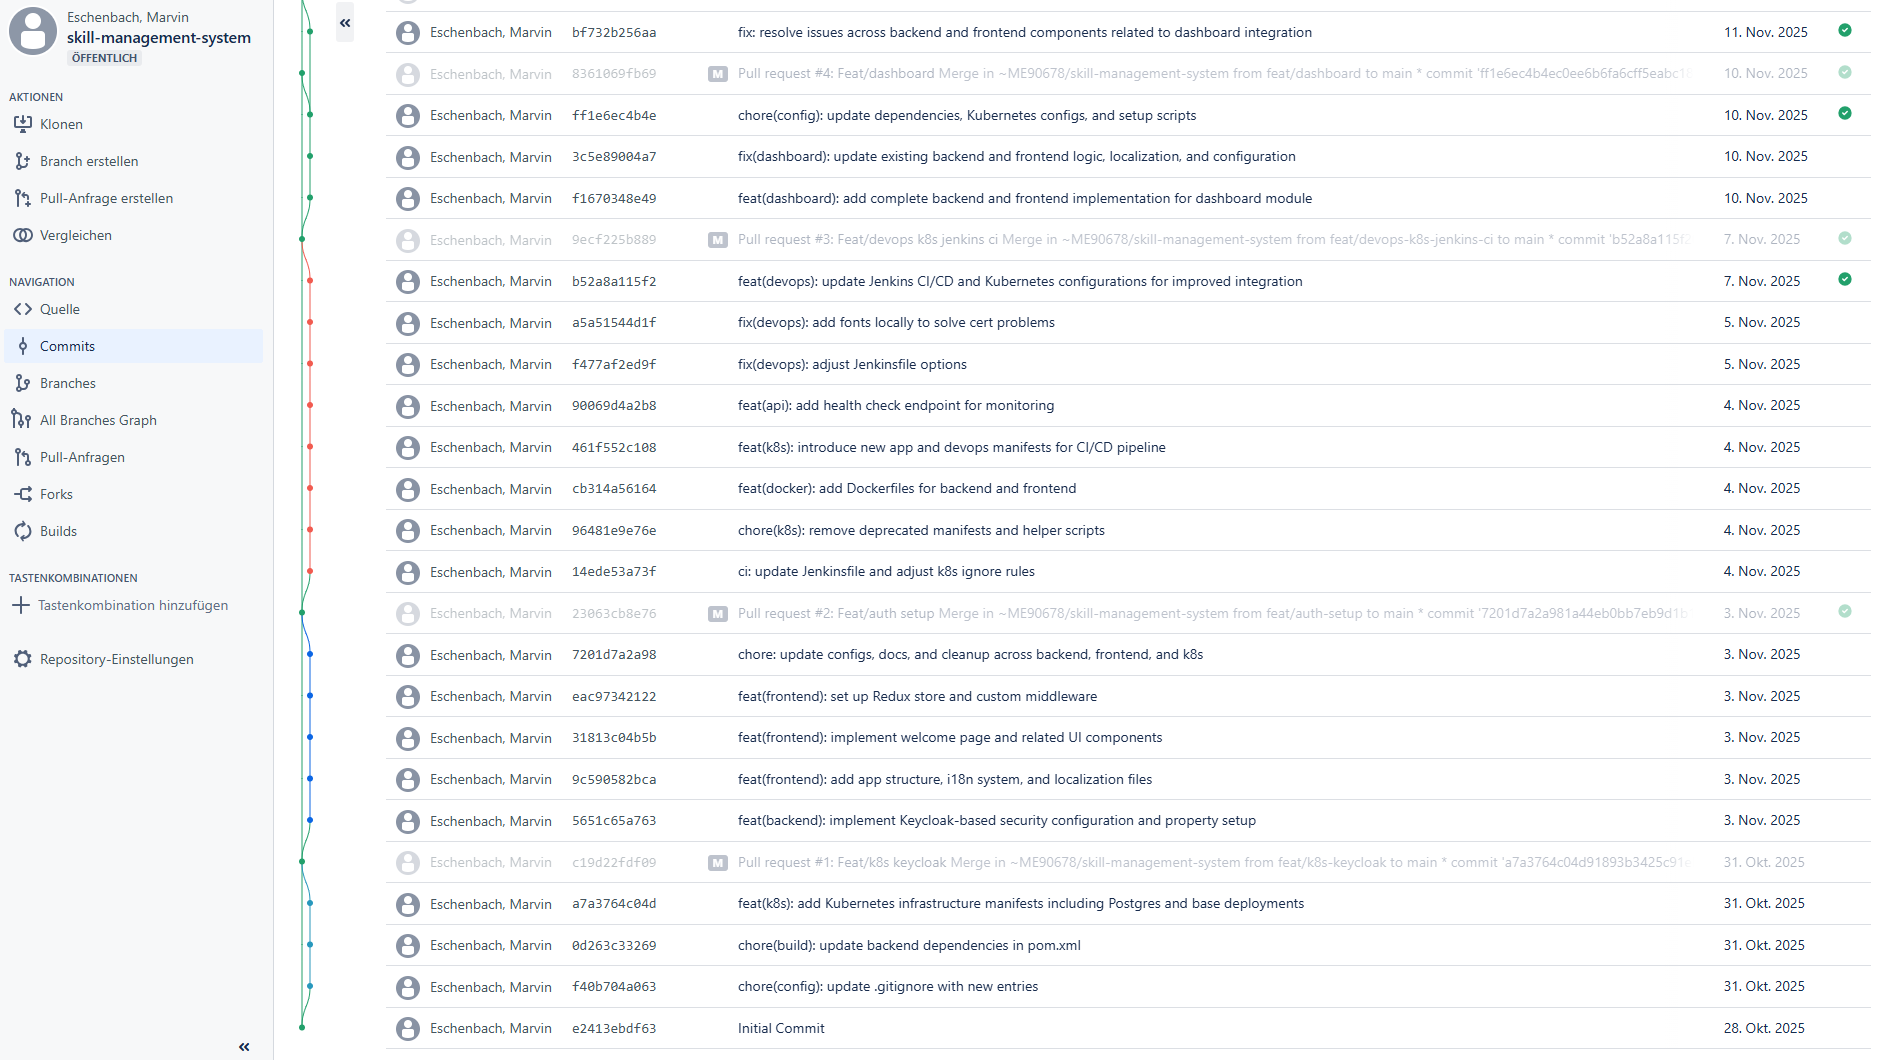
\includegraphics[width=0.95\textwidth]{references/commits.png}
\caption{Commit-Historie mit Conventional Commits und Commit Lint}
\label{fig:commits}
\end{figure}

Abbildung~\ref{fig:commits} zeigt die strukturierte Commit-Historie nach Conventional Commits-Standard mit Commit Lint-Validierung. Die Commit-Messages folgen dem Format \texttt{type(scope): description} und ermöglichen automatisches Changelog-Generation und semantische Versionierung.

\subsubsection{SonarQube Code-Analyse}

\paragraph{Backend Quality Gate}

\begin{figure}[H]
\centering
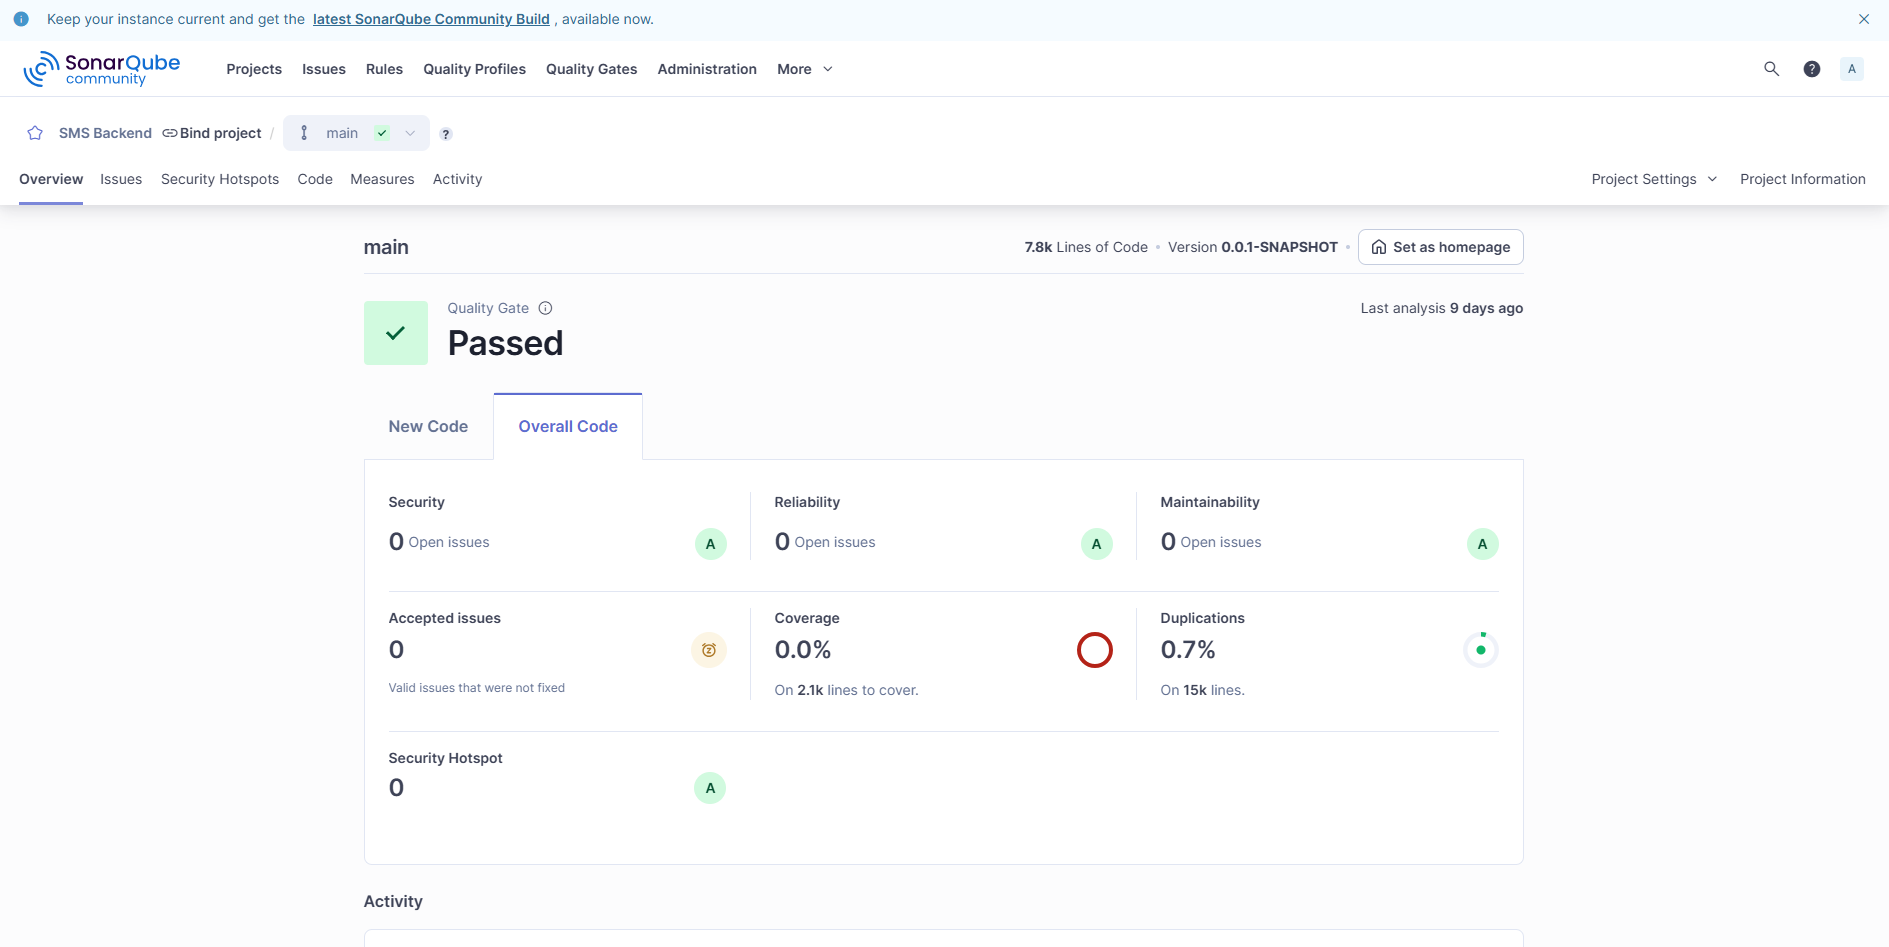
\includegraphics[width=0.95\textwidth]{references/sonar-backend.png}
\caption{SonarQube Analyse -- Backend (SMS Backend, Branch: main)}
\label{fig:sonarqube_backend}
\end{figure}

Abbildung~\ref{fig:sonarqube_backend} zeigt die SonarQube-Analyse des Backend-Projekts mit Quality Gate \textit{Passed}. Die Metriken umfassen 7.800+ Lines of Code, 0 Open Issues in allen Kategorien (Security, Reliability, Maintainability jeweils Rating A), 0.7\% Duplications und 15k Lines to Cover (bei 0\% Test Coverage).

\paragraph{Frontend Quality Gate}

\begin{figure}[H]
\centering
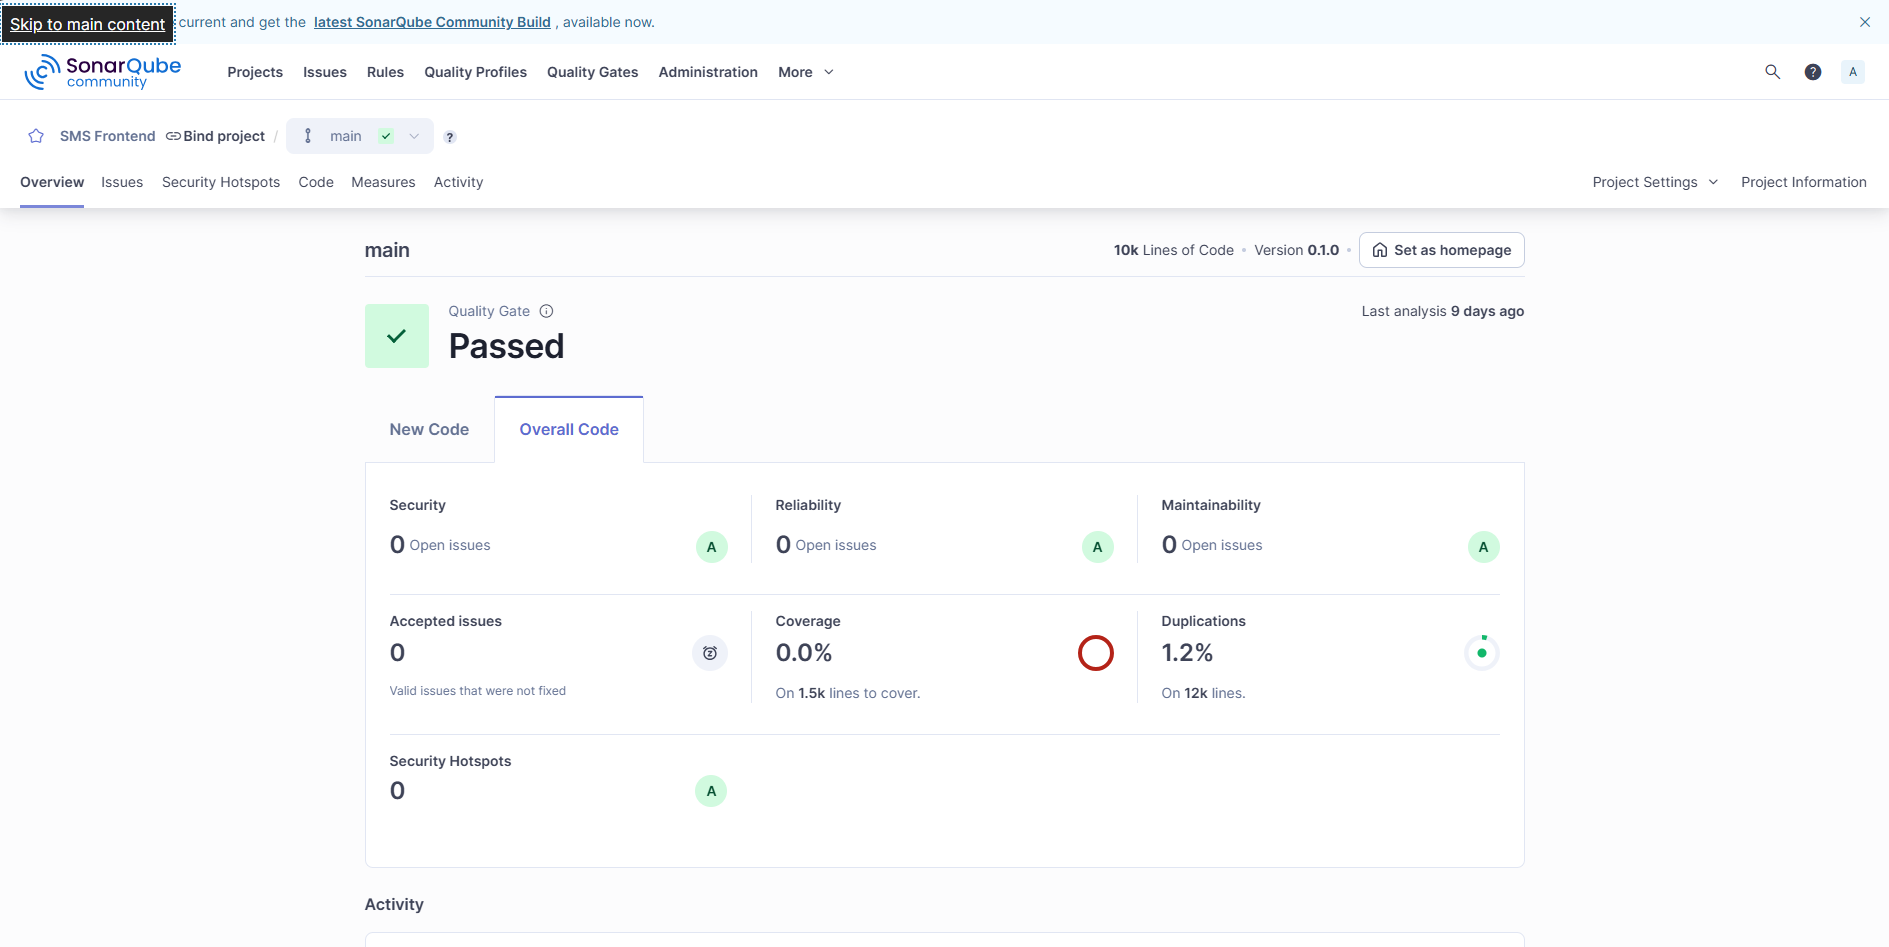
\includegraphics[width=0.95\textwidth]{references/sonar-frontend.png}
\caption{SonarQube Analyse -- Frontend (SMS Frontend, Branch: main)}
\label{fig:sonarqube_frontend}
\end{figure}

Abbildung~\ref{fig:sonarqube_frontend} zeigt die SonarQube-Analyse des Frontend-Projekts mit Quality Gate \textit{Passed}. Die Metriken umfassen 10.500+ Lines of Code, 0 Open Issues (Security/Reliability/Maintainability jeweils Rating A), 1.2\% Duplications und 12k Lines to Cover.

\subsubsection{Jenkins CI/CD Pipeline}

\begin{figure}[H]
\centering
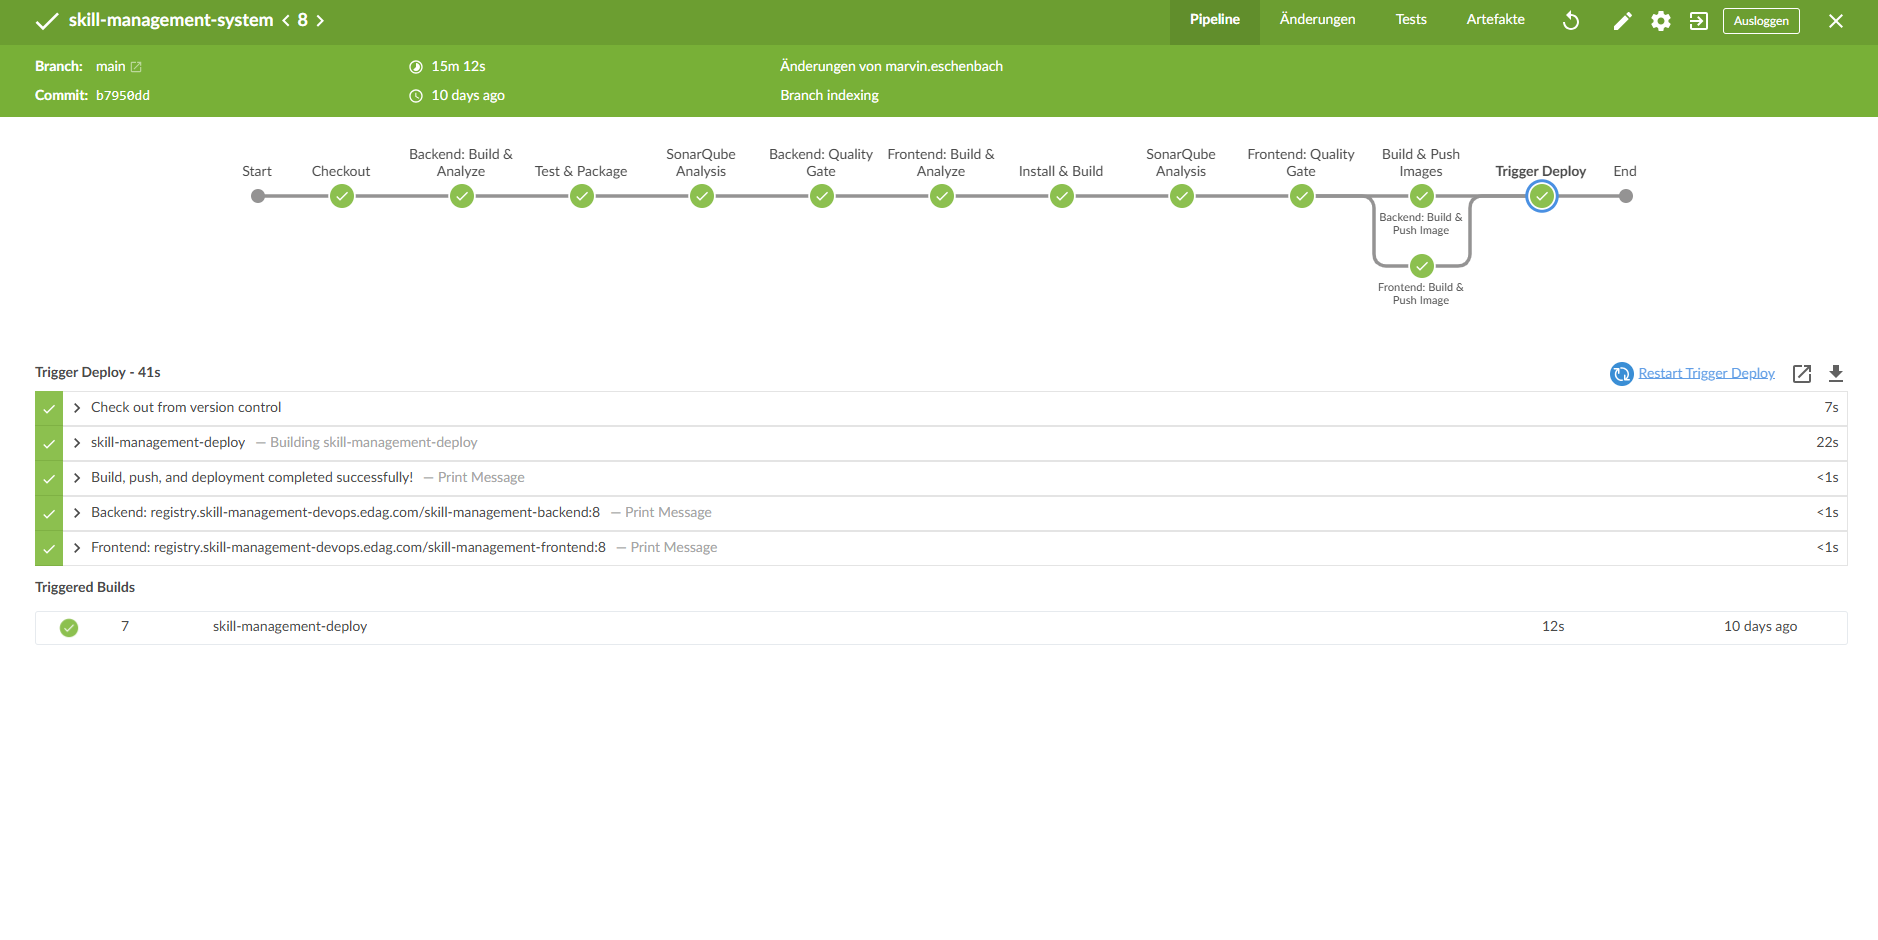
\includegraphics[width=0.95\textwidth]{references/pipeline.png}
\caption{Jenkins Declarative Pipeline -- Build \#7 (Trigger Deploy Stage)}
\label{fig:jenkins_pipeline}
\end{figure}

Abbildung~\ref{fig:jenkins_pipeline} zeigt die vollständige Jenkins Pipeline-Ausführung mit allen Stages: Checkout (7s), Backend Build \& Analyze (22s), Frontend Build \& Analyze (Build \& Push Images parallel: Backend 12s, Frontend <1s), Trigger Deploy (41s). Die Gesamtlaufzeit betrug 15 Minuten 12 Sekunden. Die Pipeline-Visualisierung zeigt den erfolgreichen Deployment-Prozess vom Branch \texttt{main} mit automatischer Image-Erstellung und Kubernetes-Deployment.

\subsubsection{Jenkinsfile Deklaration}

\begin{lstlisting}[language=bash, caption=Jenkins Declarative Pipeline -- Jenkinsfile, label=lst:jenkinsfile]
pipeline {
  agent none
  options {
    disableConcurrentBuilds()
    timeout(time: 1, unit: 'HOURS')
  }
  environment {
    REGISTRY_EXTERNAL = 'registry.skill-management-devops.edag.com'
    BACKEND_IMAGE_EXTERNAL = "\${REGISTRY_EXTERNAL}/skill-management-backend"
    FRONTEND_IMAGE_EXTERNAL = "\${REGISTRY_EXTERNAL}/skill-management-frontend"
  }
  stages {
    stage('Checkout') {
      agent { label 'universal' }
      steps { checkout scm }
    }
    stage('Backend: Build & Analyze') {
      agent { label 'backend' }
      stages {
        stage('Test & Package') {
          steps {
            container('maven') {
              sh '''#!/bin/bash
                cd backend
                ./mvnw -B clean test package
              '''
            }
          }
        }
        stage('SonarQube Analysis') {
          steps {
            container('maven') {
              withSonarQubeEnv('SonarQube') {
                sh '''cd backend
                  ./mvnw sonar:sonar \\
                    -Dsonar.projectKey=sms-backend
                '''
              }
            }
          }
        }
      }
    }
    stage('Backend: Quality Gate') {
      agent { label 'universal' }
      steps {
        timeout(time: 10, unit: 'MINUTES') {
          waitForQualityGate abortPipeline: true
        }
      }
    }
    // Frontend stages analog zu Backend
    stage('Build & Push Images') {
      when { branch 'main' }
      parallel {
        stage('Backend: Build & Push Image') {
          agent { label 'backend' }
          steps {
            container('docker') {
              script {
                docker.withRegistry(
                  "https://\${REGISTRY_EXTERNAL}", 'docker-registry') {
                  dir('backend') {
                    def img = docker.build(
                      "\${BACKEND_IMAGE_EXTERNAL}:\${BUILD_NUMBER}")
                    img.push()
                    img.push('latest')
                  }
                }
              }
            }
          }
        }
        // Frontend parallel
      }
    }
    stage('Trigger Deploy') {
      when { branch 'main' }
      agent { label 'universal' }
      steps {
        script { build job: 'skill-management-deploy' }
      }
    }
  }
}
\end{lstlisting}

Die Jenkinsfile-Konfiguration (Listing~\ref{lst:jenkinsfile}) definiert eine mehrstufige Pipeline mit Kubernetes-Agents für unterschiedliche Build-Environments (Backend: Maven, Frontend: Node.js, Docker: Image-Builds). Quality Gates stoppen die Pipeline bei SonarQube-Violations. Branch \texttt{main} triggert automatisch Docker-Image-Builds und Deployment.

\subsubsection{Lighthouse Performance Audit}

\begin{figure}[H]
\centering
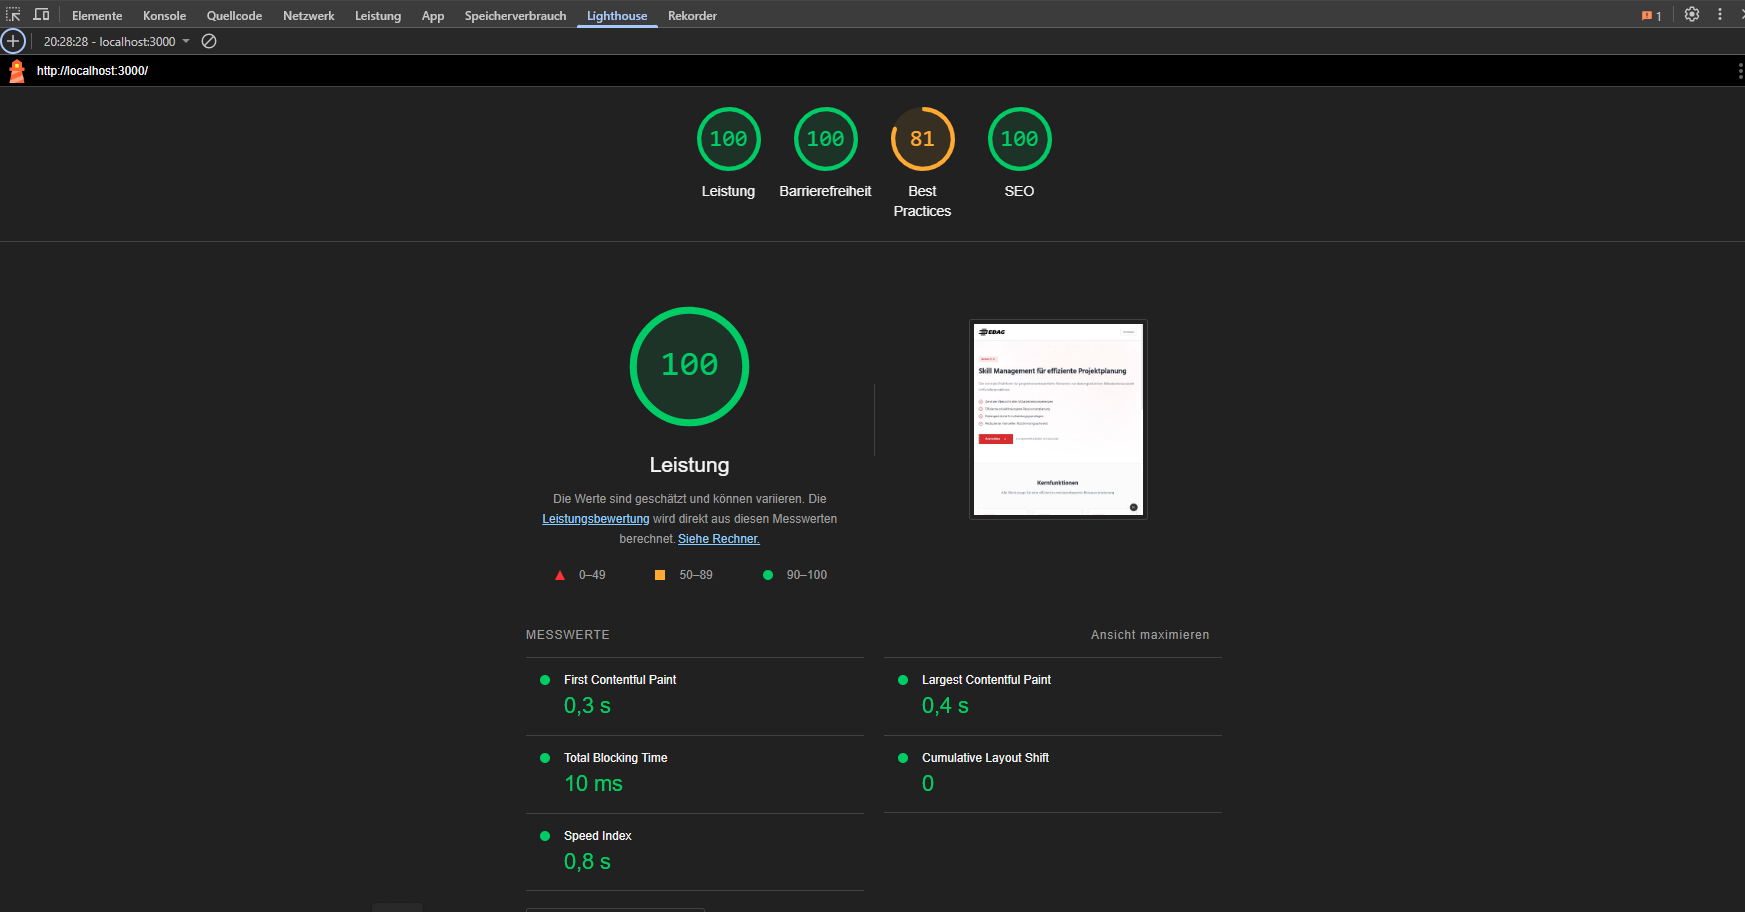
\includegraphics[width=0.90\textwidth]{references/lighthouse-welcome.png}
\caption{Google Lighthouse Audit -- Welcome Screen (Performance: 100, Best Practices: 81)}
\label{fig:lighthouse_welcome}
\end{figure}

Abbildung~\ref{fig:lighthouse_welcome} zeigt das Lighthouse-Audit\cite{lighthouse_docs} der Welcome-Seite mit exzellenten Werten: Performance 100/100 (First Contentful Paint 0.3s, Largest Contentful Paint 0.4s, Speed Index 0.8s), Accessibility 100/100, Best Practices 81/100, SEO 100/100. Die Messwerte bestätigen die Performance-Anforderungen aus Kapitel~\ref{sec:nicht_funktionale_anforderungen}.

% ==========================================
% A.4 DEPLOYMENT & KONFIGURATION
% ==========================================

\section{Deployment \& Konfiguration}

\subsection{ER-Datenmodell}
\label{sec:er_model}

\begin{figure}[H]
\centering
\begin{tikzpicture}[
    scale=1.0,
    every node/.style={transform shape},
    entity/.style={rectangle, draw, minimum width=2.5cm, minimum height=0.8cm, font=\small, align=center},
    attribute/.style={ellipse, draw, minimum width=1.5cm, minimum height=0.6cm, font=\tiny, align=center},
    key/.style={ellipse, draw, minimum width=1.5cm, minimum height=0.6cm, font=\tiny, align=center, font=\tiny\bfseries},
    relation/.style={diamond, draw, minimum width=1.8cm, minimum height=1cm, font=\scriptsize, align=center, aspect=2},
    line/.style={-}
]

% Entitäten - Optimierte Positionierung
\node[entity] (user) at (0,8) {\textbf{users}};
\node[entity] (profile) at (6,8) {\textbf{employee\_profiles}};
\node[entity] (skill) at (10,8) {\textbf{skills}};
\node[entity] (category) at (10,2) {\textbf{skill\_categories}};
\node[entity] (project) at (3,5) {\textbf{projects}};
\node[entity] (stats) at (0,3.5) {\textbf{user\_statistics}};

% Beziehungen (Rauten)
\node[relation] (r1) at (3,8) {has};
\node[relation] (r2) at (8.5,6.5) {possesses};
\node[relation] (r3) at (12,4) {belongs\\to};
\node[relation] (r4) at (1.5,6.5) {owns};
\node[relation] (r5) at (6,4) {contains};
\node[relation] (r6) at (0,5.5) {tracks};

% Primärschlüssel (PK)
\node[key] (user_id) at (-1,7.1) {\underline{id}};
\node[key] (profile_id) at (5,7) {\underline{user\_id}};
\node[key] (skill_id) at (12.2,8) {\underline{id}};
\node[key] (cat_id) at (12.5,2) {\underline{id}};
\node[key] (proj_id) at (2.5,4) {\underline{id}};
\node[key] (stats_id) at (0,2.5) {\underline{user\_id}};

% Fremdschlüssel (FK)
\node[attribute] (skill_cat_fk) at (12,7) {category\_id};
\node[attribute] (proj_created_fk) at (3.5,6) {created\_by\\\_user\_id};

% Attribute employee_skills (m:n)
\node[key] (es_emp) at (7.5,4.9) {\underline{employee\_id}};
\node[key] (es_skill) at (10.5,4.9) {\underline{skill\_id}};
\node[attribute] (es_id) at (9,5.5) {id};

% Attribute project_members (m:n)
\node[key] (pm_proj) at (4.5,3) {\underline{project\_id}};
\node[key] (pm_emp) at (8,3) {\underline{employee\_id}};
\node[attribute] (pm_id) at (6,2.2) {id};

% Verbindungen Entitäten zu Attributen
\draw[line] (user) -- (user_id);
\draw[line] (profile) -- (profile_id);
\draw[line] (skill) -- (skill_id);
\draw[line] (skill) -- (skill_cat_fk);
\draw[line] (category) -- (cat_id);
\draw[line] (project) -- (proj_id);
\draw[line] (project) -- (proj_created_fk);
\draw[line] (stats) -- (stats_id);

% Verbindungen m:n-Beziehungen zu Attributen
\draw[line] (r2) -- (es_emp);
\draw[line] (r2) -- (es_skill);
\draw[line] (r2) -- (es_id);
\draw[line] (r5) -- (pm_proj);
\draw[line] (r5) -- (pm_emp);
\draw[line] (r5) -- (pm_id);

% Beziehungen mit Kardinalitäten
\draw[line] (user) -- node[above, font=\small] {1} (r1);
\draw[line] (r1) -- node[above, font=\small] {1} (profile);

\draw[line] (profile) -- node[above left, font=\small] {n} (r2);
\draw[line] (r2) -- node[above right, font=\small] {m} (skill);

\draw[line] (skill) -- node[right, font=\small] {n} (r3);
\draw[line] (r3) -- node[right, font=\small] {1} (category);

\draw[line] (user) -- node[left, font=\small] {1} (r4);
\draw[line] (r4) -- node[left, font=\small] {n} (project);

\draw[line] (project) -- node[above, font=\small] {n} (r5);
\draw[line] (r5) -- node[below right, font=\small] {m} (profile);

\draw[line] (user) -- node[left, font=\small] {1} (r6);
\draw[line] (r6) -- node[left, font=\small] {1} (stats);

\end{tikzpicture}
\caption{Entity-Relationship-Diagramm nach UML-Standard (Kernentitäten)}
\label{fig:erd}
\end{figure}

\subsubsection{Datenbankmodell}

Abbildung~\ref{fig:db_screenshot} zeigt die tatsächliche Datenbankstruktur mit allen 15 Tabellen (14 Anwendungstabellen + \texttt{flyway\_schema\_history}), ihren Spalten, Datentypen und Constraints.

\begin{figure}[H]
\centering
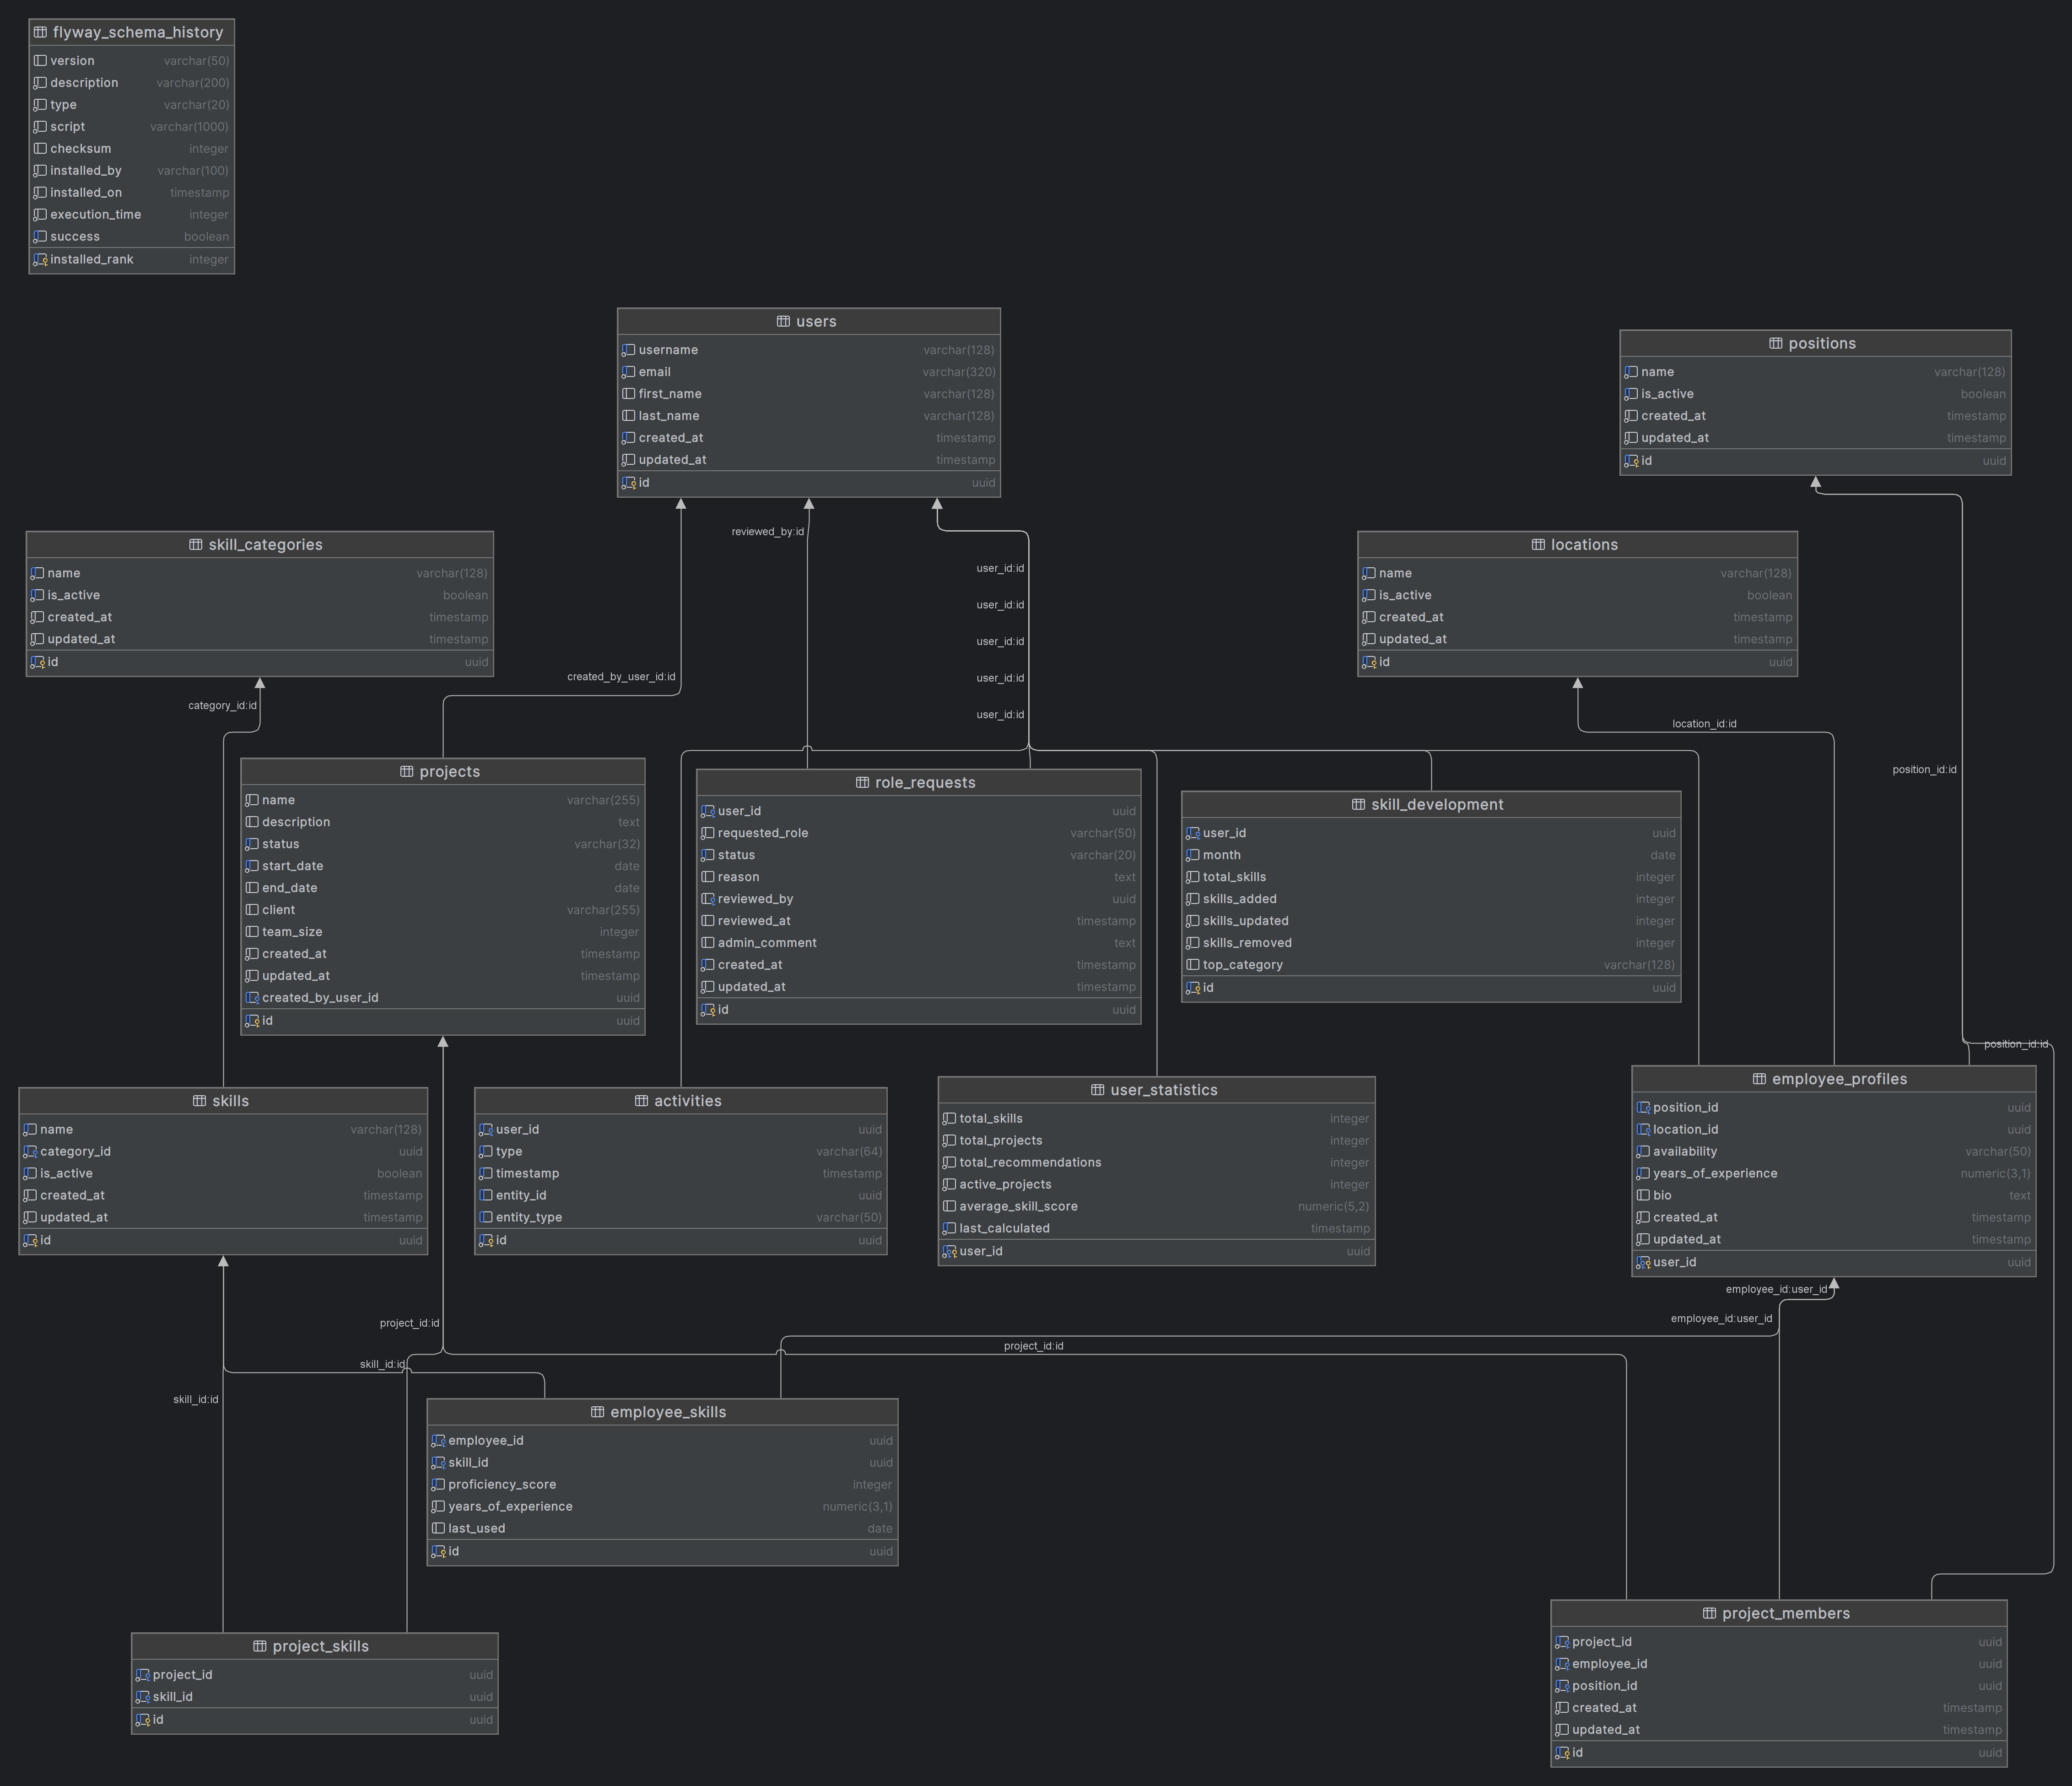
\includegraphics[width=0.95\textwidth]{references/skillmanagement@localhost.png}
\caption{Datenbank-Schema: Vollständige Tabellenstruktur mit 15 Tabellen}
\label{fig:db_screenshot}
\end{figure}

\subsection{Datenbank-Migrationen}
\label{sec:db_migrations}

Die 15 Flyway-Migrationsskripte dokumentieren die vollständige Datenbank-Evolution von Basis-Tabellen über automatisierte Trigger bis zu umfassenden Analytics. Die versionierte Schema-Migration gewährleistet reproduzierbare Deployments und nachvollziehbare Änderungen.

\subsubsection{Migrations-Übersicht}

\begin{table}[H]
\centering
\footnotesize
\rowcolors{2}{EDAGDunkelgrau!10}{white}
\begin{tabularx}{\textwidth}{|l|l|X|r|}
\hline
\rowcolor{EDAGDunkelgrau!10}
\textbf{Nr.} & \textbf{Kategorie} & \textbf{Beschreibung} & \textbf{LOC} \\
\hline
V1 & Schema & users, positions, locations, skill\_categories, skills & 92 \\
\hline
V2 & Schema & employee\_profiles, employee\_skills (Junction) & 56 \\
\hline
V3 & Schema & projects, project\_skills, project\_positions & 143 \\
\hline
V4 & Analytics & user\_statistics, skill\_development, activities & 102 \\
\hline
V5 & Trigger & Automatische updated\_at-Timestamps (7 Tabellen) & 48 \\
\hline
V6 & Trigger & Echtzeit-Aggregation: total\_skills, avg\_score, project\_counts & 131 \\
\hline
V7 & Trigger & Audit-Trail: SKILL\_ADDED, PROJECT\_CREATED, PROFILE\_UPDATED & 134 \\
\hline
V8 & Trigger & Monatliche Skill-Entwicklung Snapshots & 177 \\
\hline
V9 & Daten & 200+ Skills, 55+ Positionen, 30 Standorte & 379 \\
\hline
V10 & Trigger & Auto-Erstellung employee\_profiles bei User-Insert & 47 \\
\hline
V11 & Refactoring & project\_members n:m-Tabelle (eliminiert Redundanz) & 278 \\
\hline
V12 & Trigger & Automatische Team-Size-Berechnung & 36 \\
\hline
V13 & Refactoring & Entfernung team\_size CHECK-Constraint & 7 \\
\hline
V14 & Schema & role\_requests (Self-Service Rollenanfragen) & 38 \\
\hline
V15 & Trigger & 30+ Event-Typen: ROLE\_REQUEST\_APPROVED, PROJECT\_MEMBER\_ADDED & 358 \\
\hline
\rowcolor{EDAGDunkelgrau!30}
\textbf{Gesamt} & \textbf{15 Dateien} & \textbf{Vollständig versioniertes Datenbankschema} & \textbf{2.026} \\
\hline
\end{tabularx}
\caption{Vollständige Übersicht aller Flyway-Datenbank-Migrationen}
\label{tab:db_migrations}
\end{table}

\paragraph{Beispiel-Listings}

Die folgenden Auszüge zeigen exemplarisch die Struktur der ersten zwei Migrationen. Alle weiteren 13 Migrationen folgen dem gleichen Schema mit vollständiger Dokumentation durch SQL-Kommentare.

\subparagraph{V1: Basis-Tabellen (Auszug)}\mbox{}\vspace{4pt}

\begin{lstlisting}[language=SQL, basicstyle=\scriptsize\ttfamily, frame=single]
-- V1__create_base_tables.sql
CREATE EXTENSION IF NOT EXISTS pg_trgm; -- Full-text search

CREATE TABLE users (
    id UUID PRIMARY KEY DEFAULT gen_random_uuid(),
    username VARCHAR(128) NOT NULL UNIQUE,
    email VARCHAR(320) NOT NULL UNIQUE,
    first_name VARCHAR(128),
    last_name VARCHAR(128),
    created_at TIMESTAMP NOT NULL DEFAULT CURRENT_TIMESTAMP
);

CREATE TABLE skills (
    id UUID PRIMARY KEY DEFAULT gen_random_uuid(),
    name VARCHAR(128) NOT NULL UNIQUE,
    category_id UUID NOT NULL,
    CONSTRAINT fk_skills_category FOREIGN KEY (category_id)
        REFERENCES skill_categories(id) ON DELETE RESTRICT
);
\end{lstlisting}

\subparagraph{V2: Employee Skills Junction-Tabelle (Auszug)}\mbox{}\vspace{4pt}

\begin{lstlisting}[language=SQL, basicstyle=\scriptsize\ttfamily, frame=single]
-- V2__create_employee_profiles.sql
CREATE TABLE employee_skills (
    id UUID PRIMARY KEY DEFAULT gen_random_uuid(),
    employee_id UUID NOT NULL,
    skill_id UUID NOT NULL,
    proficiency_score INTEGER NOT NULL,
    CONSTRAINT fk_employee_skill_employee FOREIGN KEY (employee_id)
        REFERENCES employee_profiles(user_id) ON DELETE CASCADE,
    CONSTRAINT chk_proficiency_score CHECK 
        (proficiency_score >= 0 AND proficiency_score <= 100)
);
\end{lstlisting}

\vspace{1em}

\noindent\textbf{Repository-Pfad:} Alle 15 vollständigen SQL-Migrationsskripte (2.026 LOC) sind verfügbar unter:\\ 
\texttt{backend/src/main/resources/db/migration/V*.sql}

\subsection{Kubernetes Ingress-Konfiguration}

\begin{table}[H]
\centering
\footnotesize
\rowcolors{2}{EDAGDunkelgrau!10}{white}
\begin{tabularx}{\textwidth}{|p{4.5cm}|p{3cm}|X|}
\hline
\rowcolor{EDAGDunkelgrau!10}
\textbf{Hostname} & \textbf{Service} & \textbf{Beschreibung} \\
\hline
keycloak.dev.local & keycloak:8080 & Identity Provider (Dev) \\
\hline
skill-management.edag.com & frontend:3000 & Next.js Frontend (Prod) \\
\hline
api.skill-management.edag.com & backend:8080 & Spring Boot Backend (Prod) \\
\hline
keycloak.skill-management.edag.com & keycloak:8080 & Keycloak IAM (Prod) \\
\hline
jenkins.devops.local & jenkins:8080 & CI/CD Pipeline \\
\hline
sonarqube.devops.local & sonarqube:9000 & Code-Qualität \\
\hline
registry.devops.local & docker-registry:5000 & Docker Registry \\
\hline
\end{tabularx}
\caption{Traefik Ingress-Konfiguration für alle Environments}
\label{tab:ingress_config}
\end{table}

% ==========================================
% A.5 DOKUMENTATION
% ==========================================

\section{Dokumentation}

\subsection{UI-Screenshots}
\label{sec:ui_screenshots}

\subsubsection{Authentifizierung und Onboarding}

\begin{figure}[H]
\centering
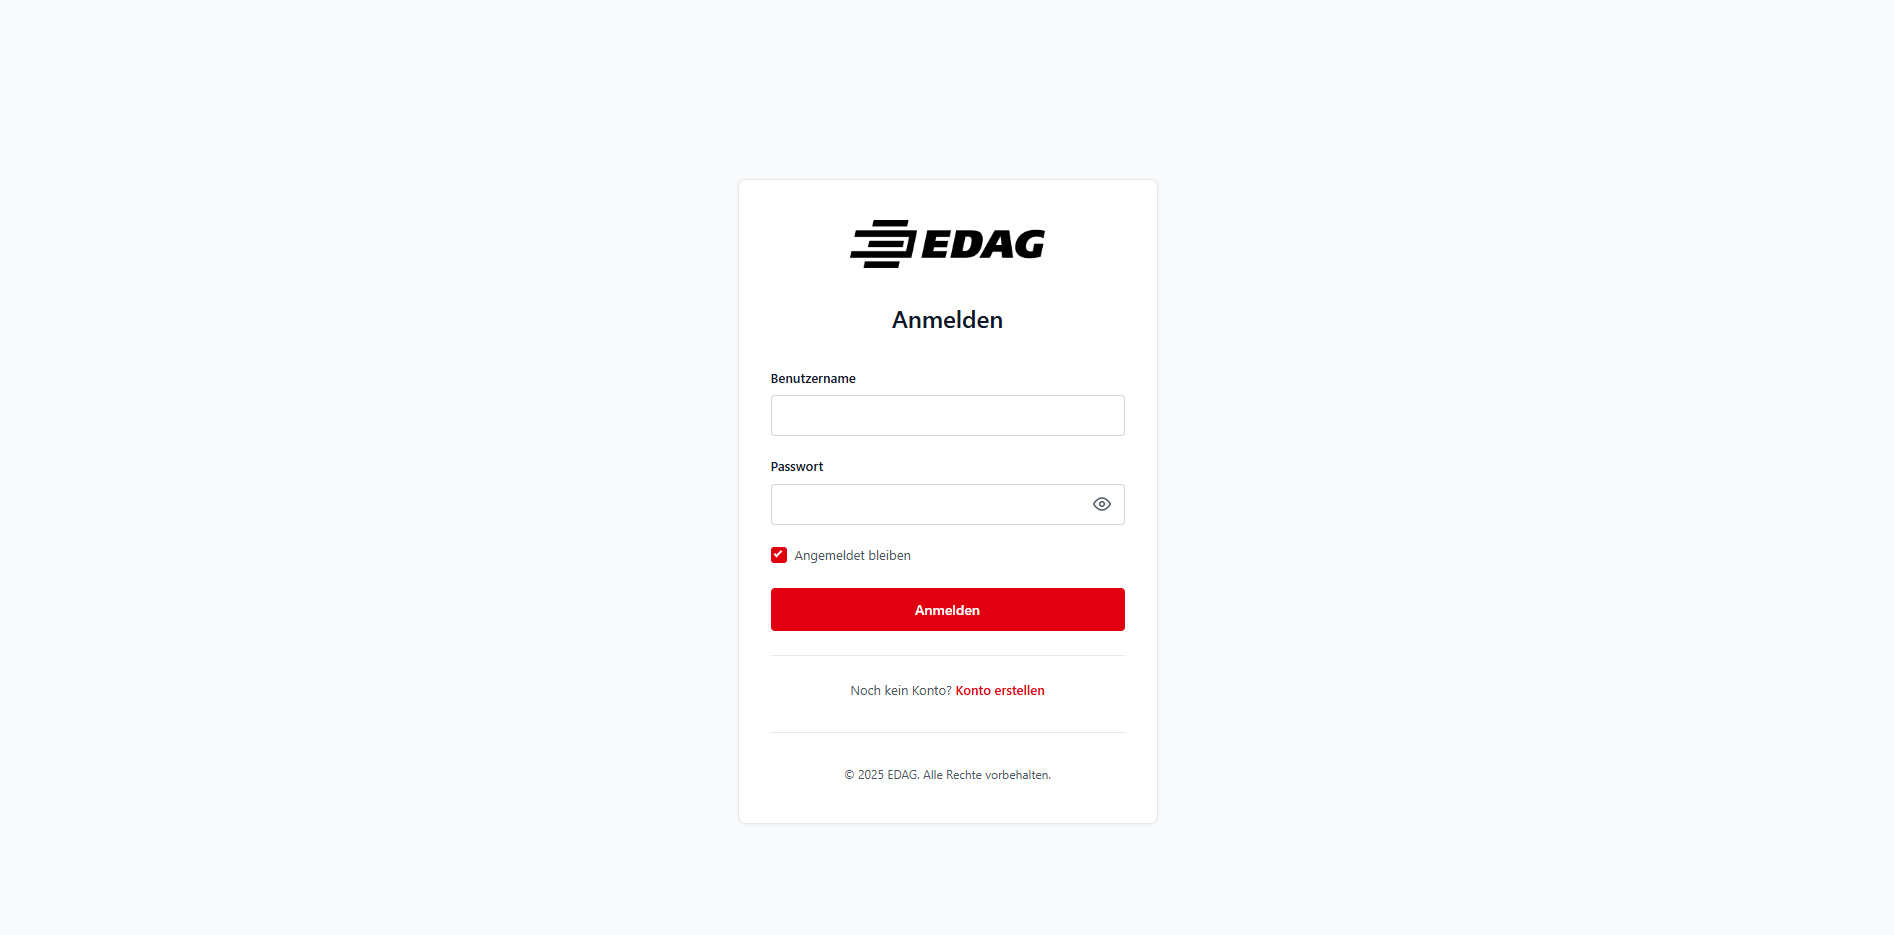
\includegraphics[width=0.9\textwidth]{references/ui-login-1.png}
\caption{Login-Seite mit Keycloak OAuth2/OIDC-Integration}
\label{fig:ui_login_1}
\end{figure}

\begin{figure}[H]
\centering
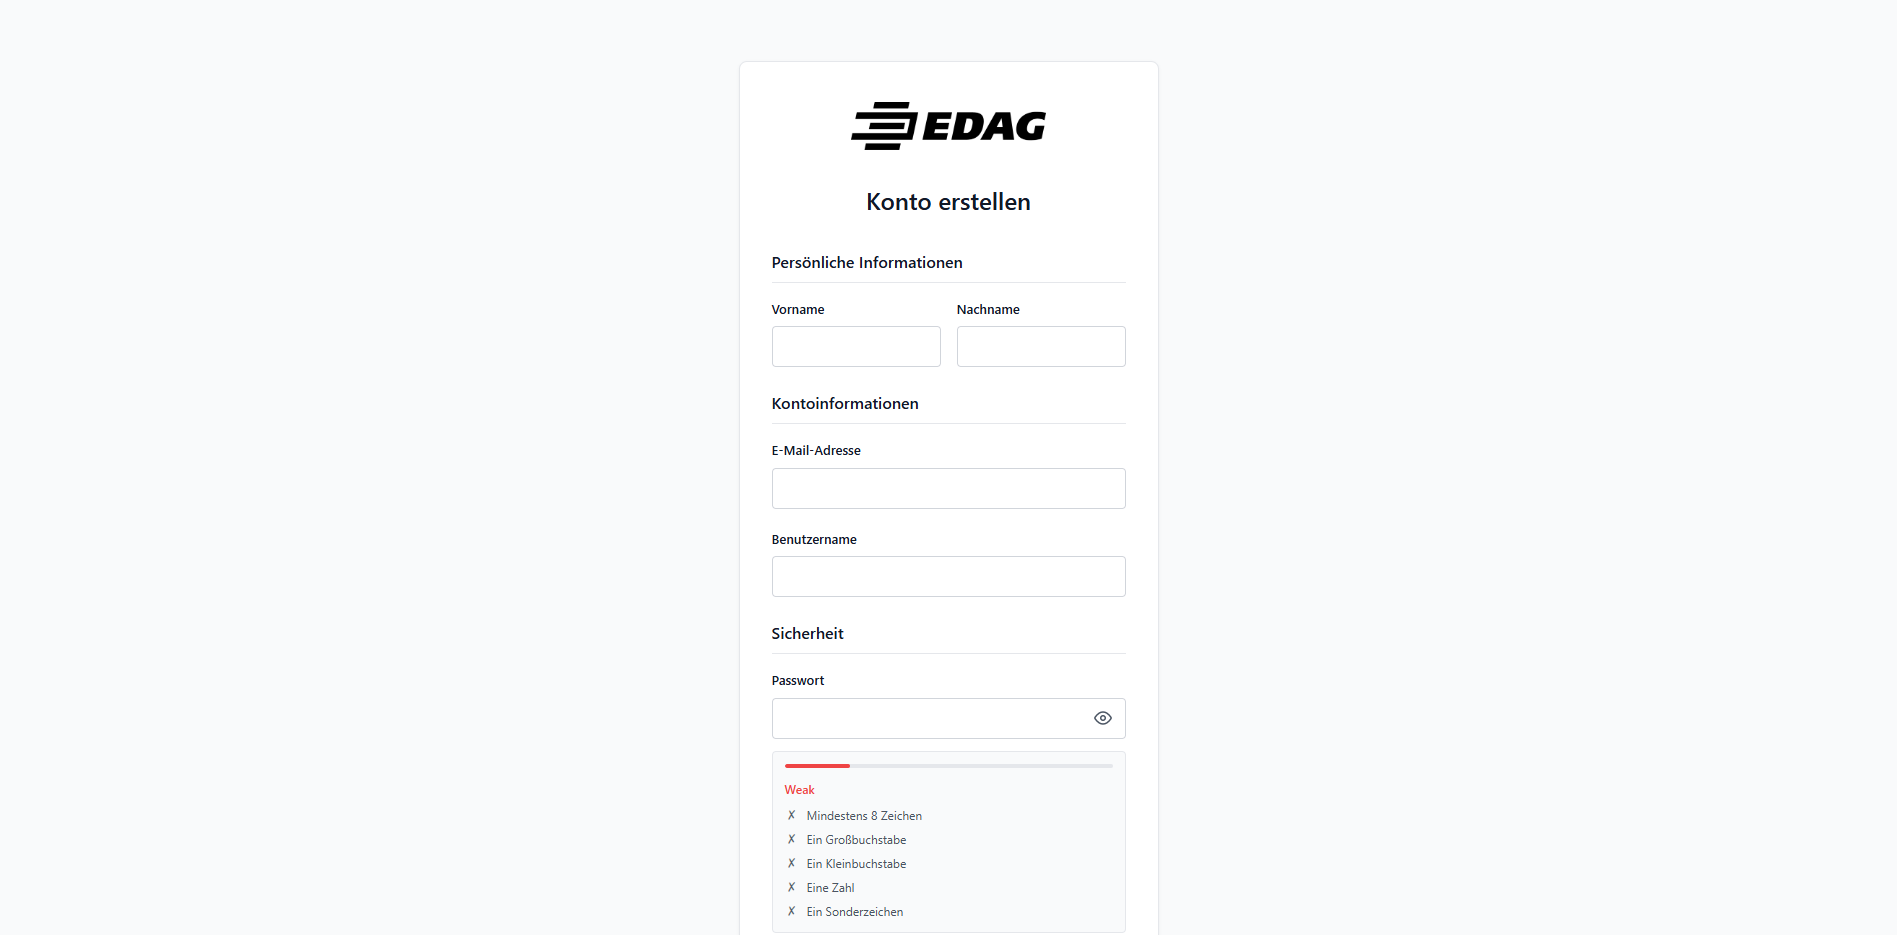
\includegraphics[width=0.9\textwidth]{references/ui-login-2.png}
\caption{Keycloak-Authentifizierungsmaske}
\label{fig:ui_login_2}
\end{figure}

\begin{figure}[H]
\centering
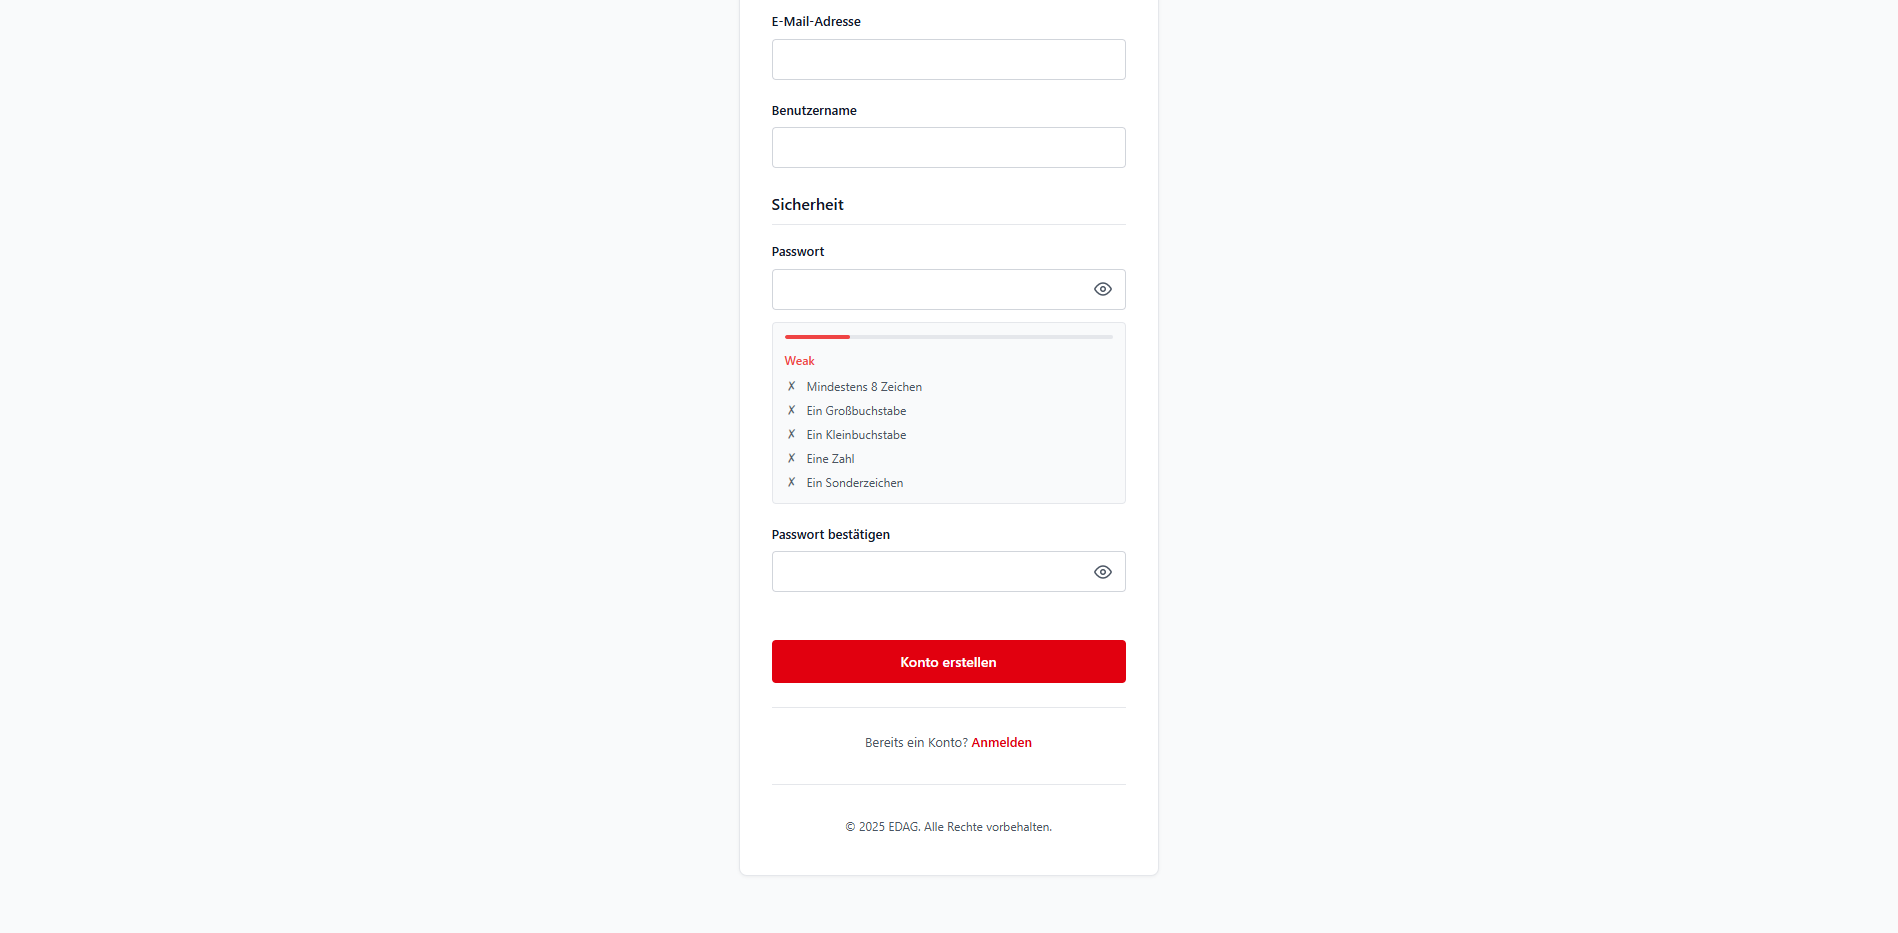
\includegraphics[width=0.9\textwidth]{references/ui-login-3.png}
\caption{Login-Erfolgsmeldung und Weiterleitung}
\label{fig:ui_login_3}
\end{figure}

\begin{figure}[H]
\centering
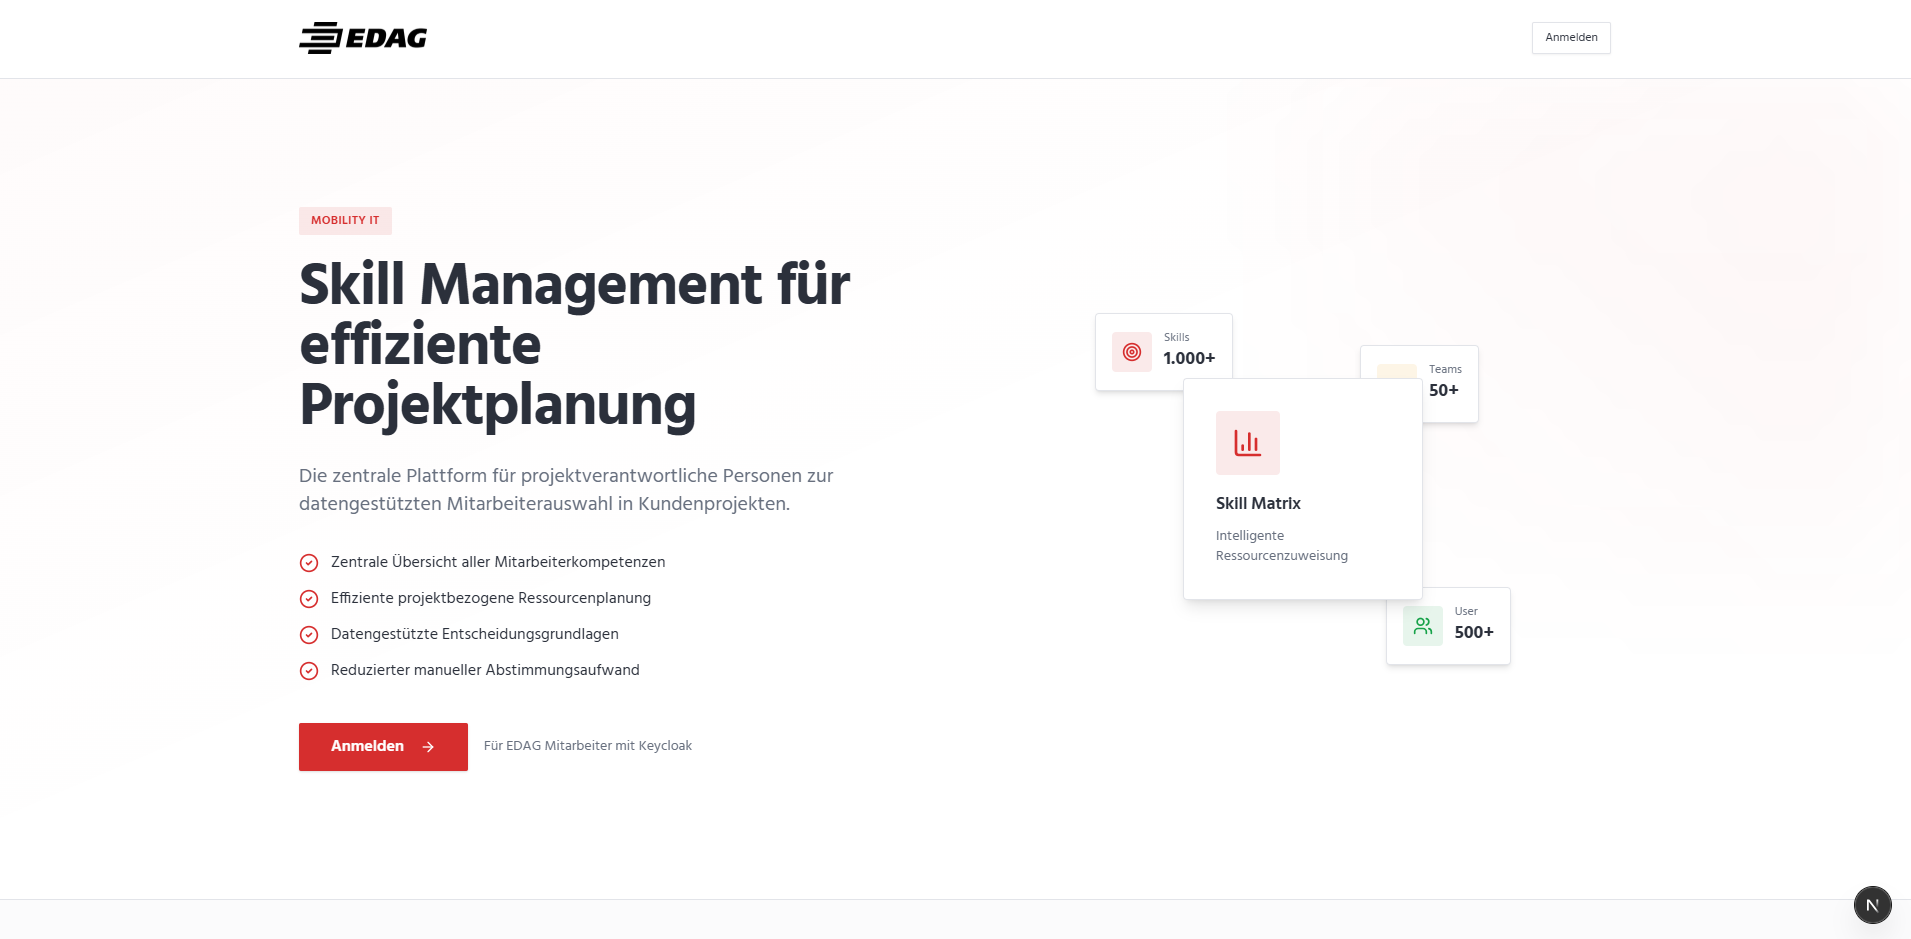
\includegraphics[width=0.9\textwidth]{references/ui-welcome-1.png}
\caption{Welcome-Seite: Erste Schritte nach Registrierung}
\label{fig:ui_welcome_1}
\end{figure}

\begin{figure}[H]
\centering
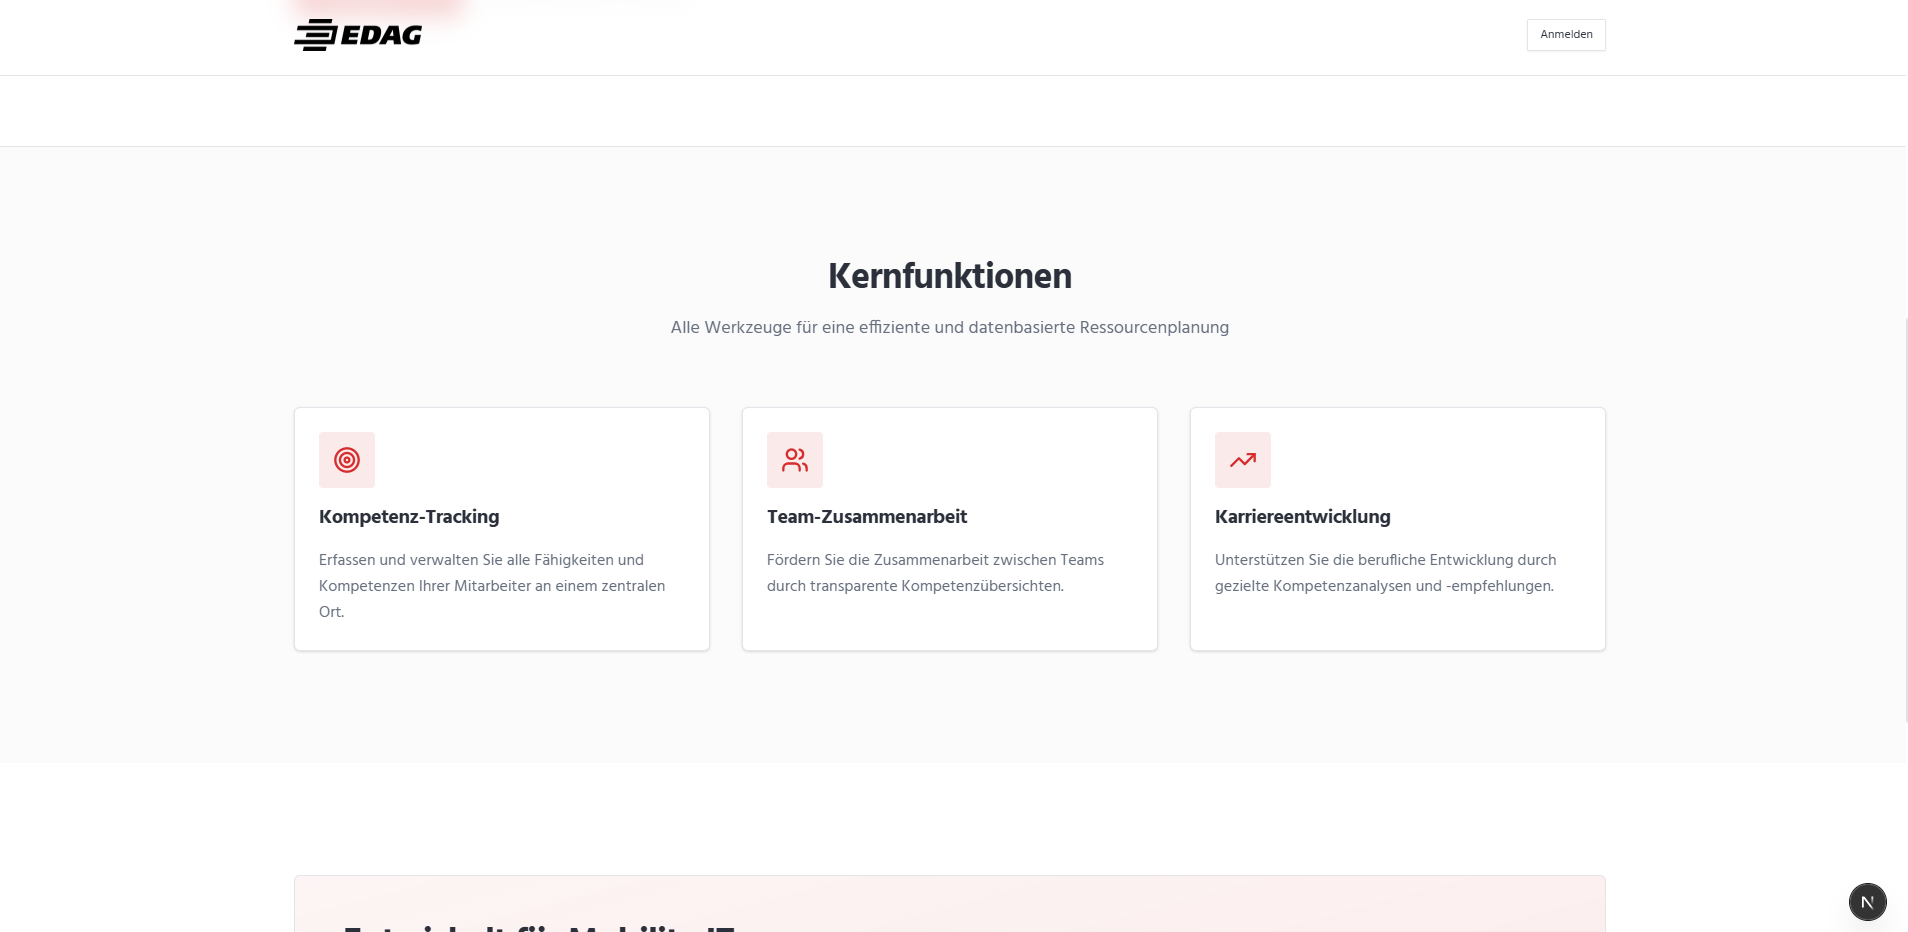
\includegraphics[width=0.9\textwidth]{references/ui-welcome-2.png}
\caption{Welcome-Seite: Profilkonfiguration}
\label{fig:ui_welcome_2}
\end{figure}

\begin{figure}[H]
\centering
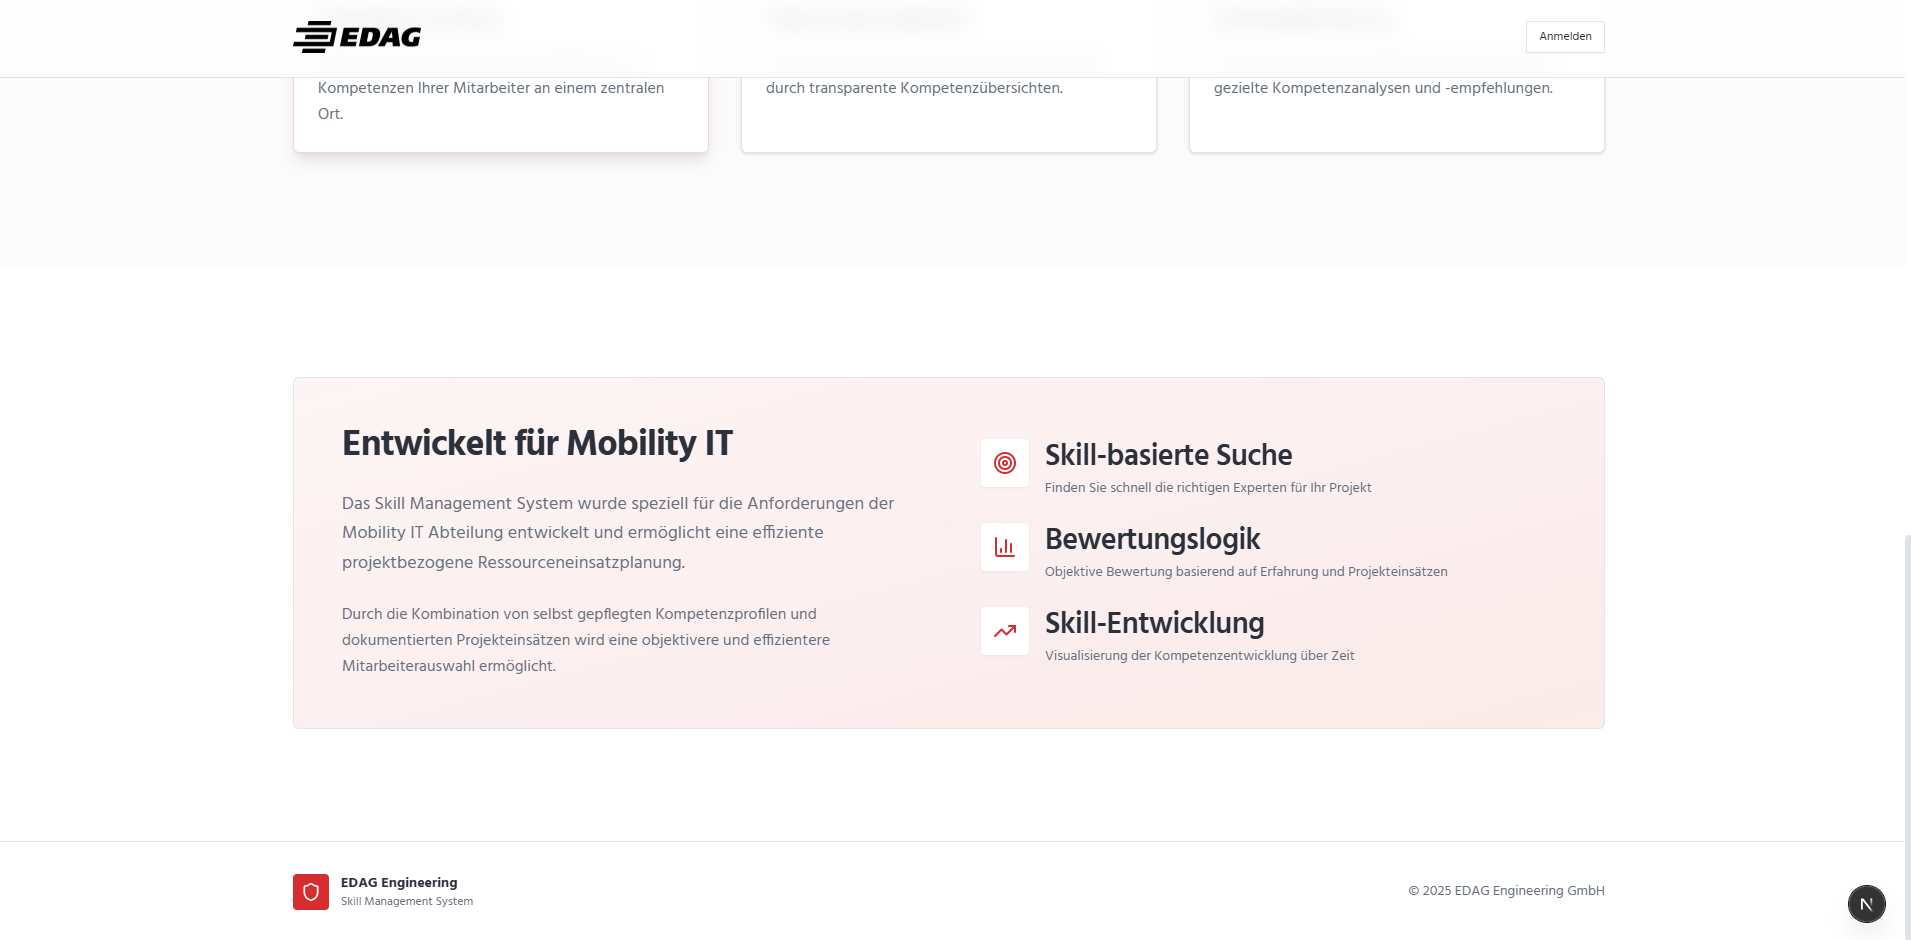
\includegraphics[width=0.9\textwidth]{references/ui-welcome-3.png}
\caption{Welcome-Seite: Skill-Auswahl}
\label{fig:ui_welcome_3}
\end{figure}

\subsubsection{Dashboard und Home}

\begin{figure}[H]
\centering
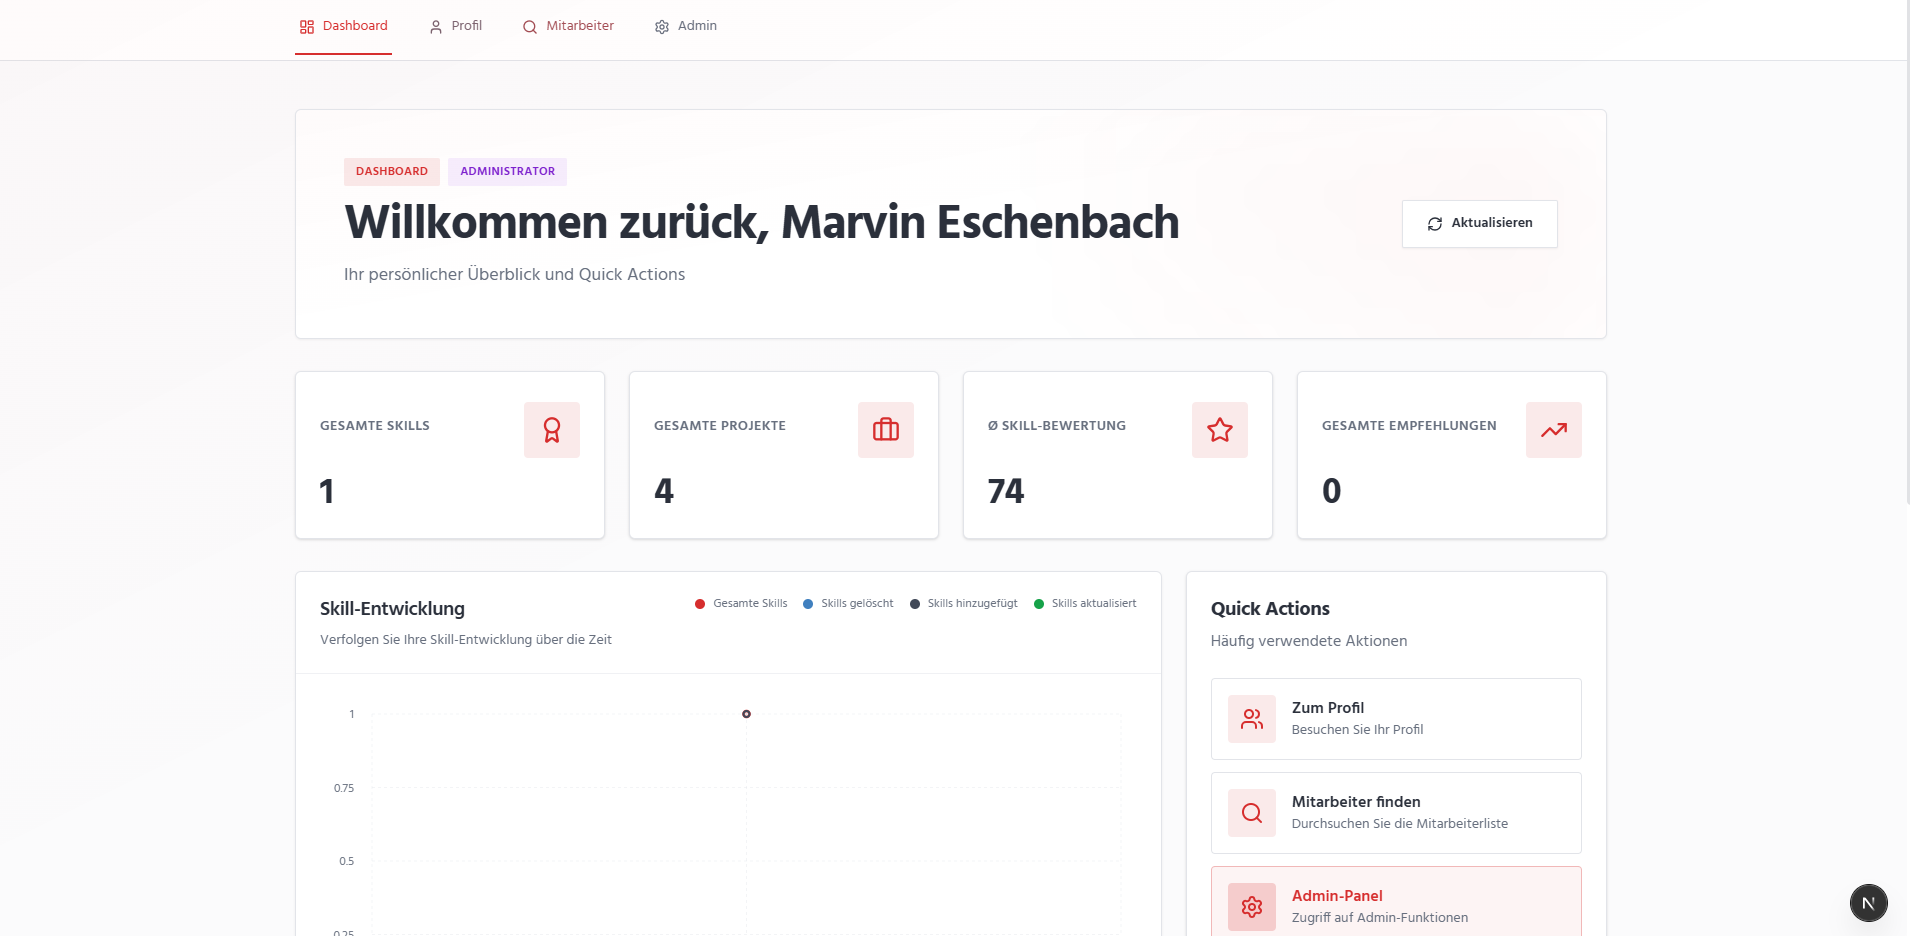
\includegraphics[width=\textwidth]{references/ui-home-1.png}
\caption{Dashboard-Übersicht mit personalisierten Kennzahlen}
\label{fig:ui_home_1}
\end{figure}

\begin{figure}[H]
\centering
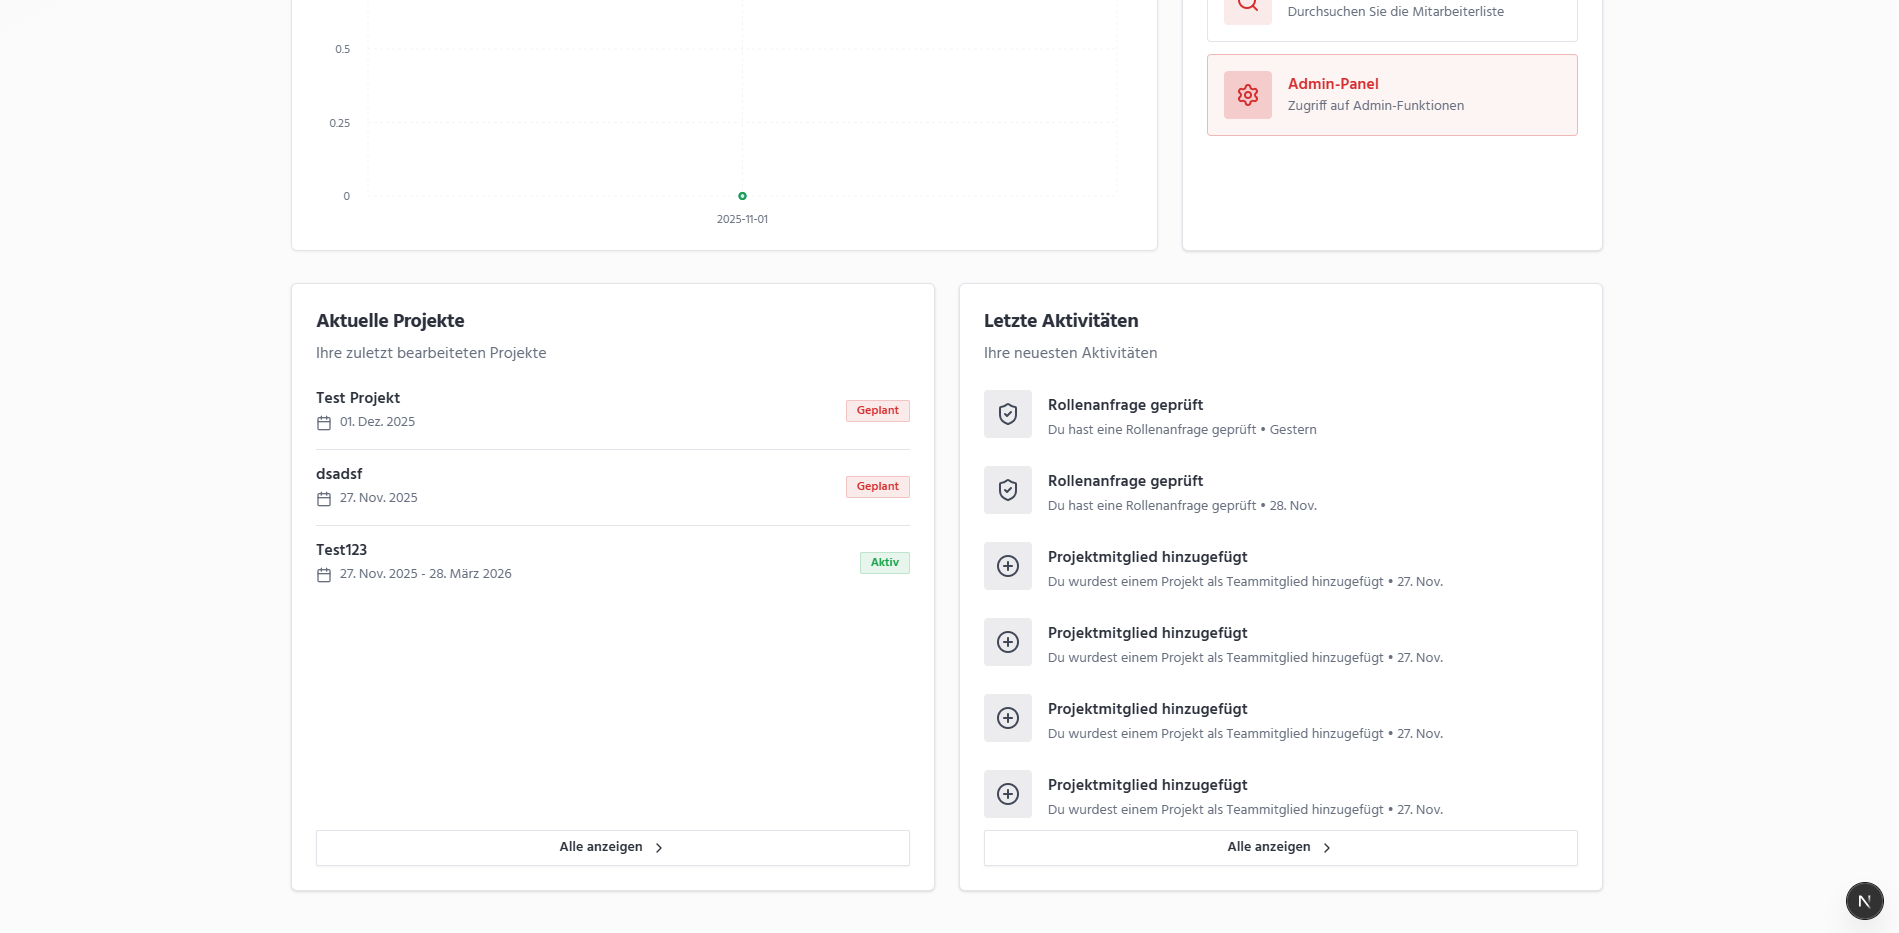
\includegraphics[width=\textwidth]{references/ui-home-2.png}
\caption{Dashboard mit Skill-Entwicklungstrends}
\label{fig:ui_home_2}
\end{figure}

\subsubsection{Profilverwaltung}

\begin{figure}[H]
\centering
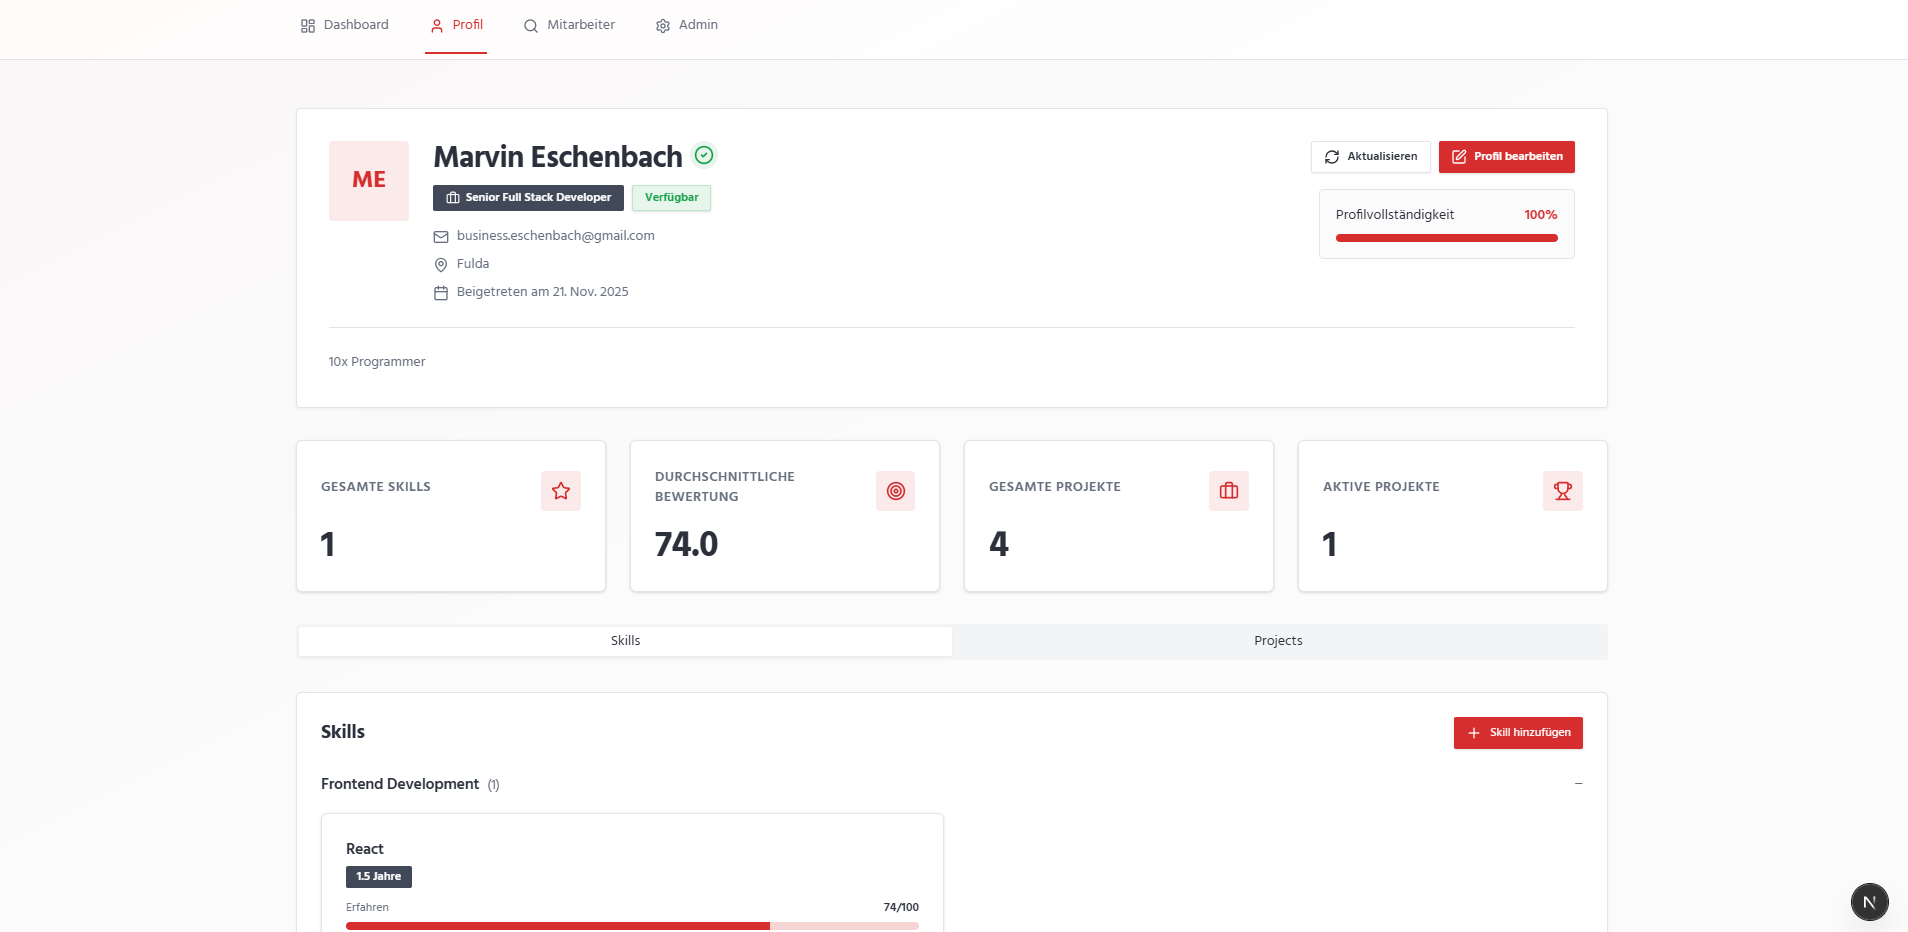
\includegraphics[width=\textwidth]{references/ui-profile-1.png}
\caption{Profil-Bearbeitung: Persönliche Daten und Skills}
\label{fig:ui_profile_1}
\end{figure}

\begin{figure}[H]
\centering
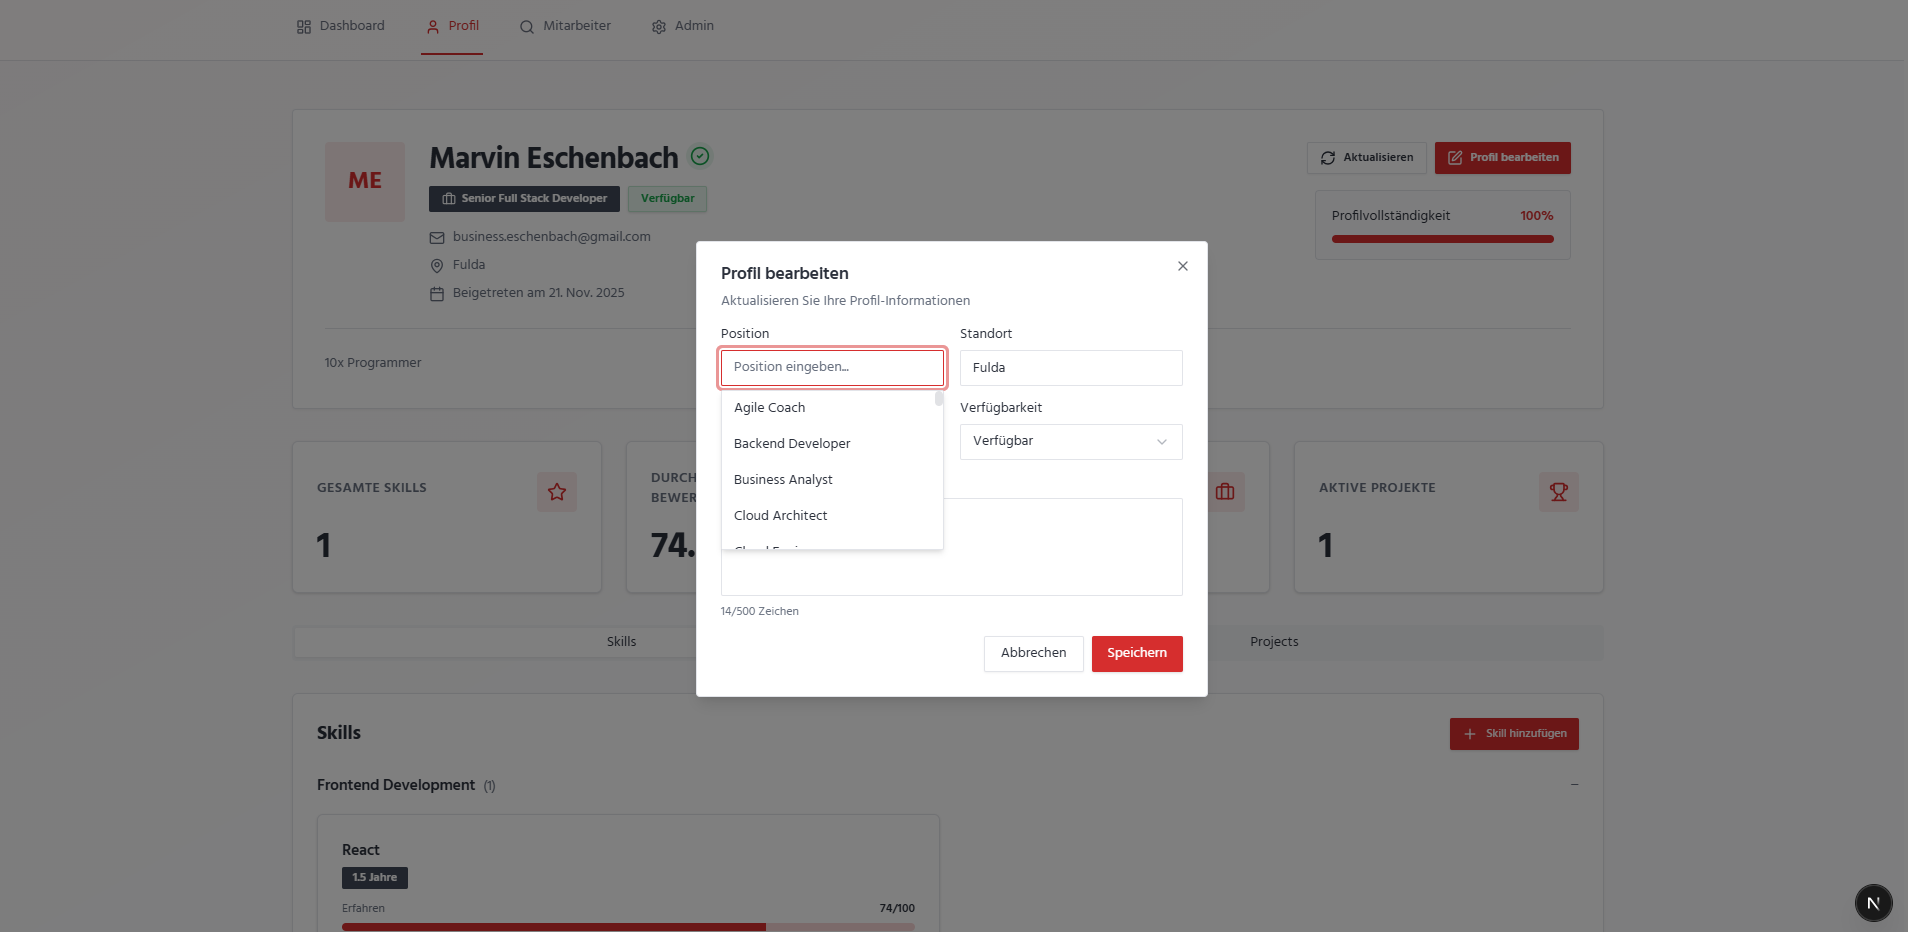
\includegraphics[width=\textwidth]{references/ui-profile-2.png}
\caption{Profil-Ansicht: Skill-Matrix mit Proficiency-Scores}
\label{fig:ui_profile_2}
\end{figure}

\subsubsection{Mitarbeiter- und Projektsuche}

\begin{figure}[H]
\centering
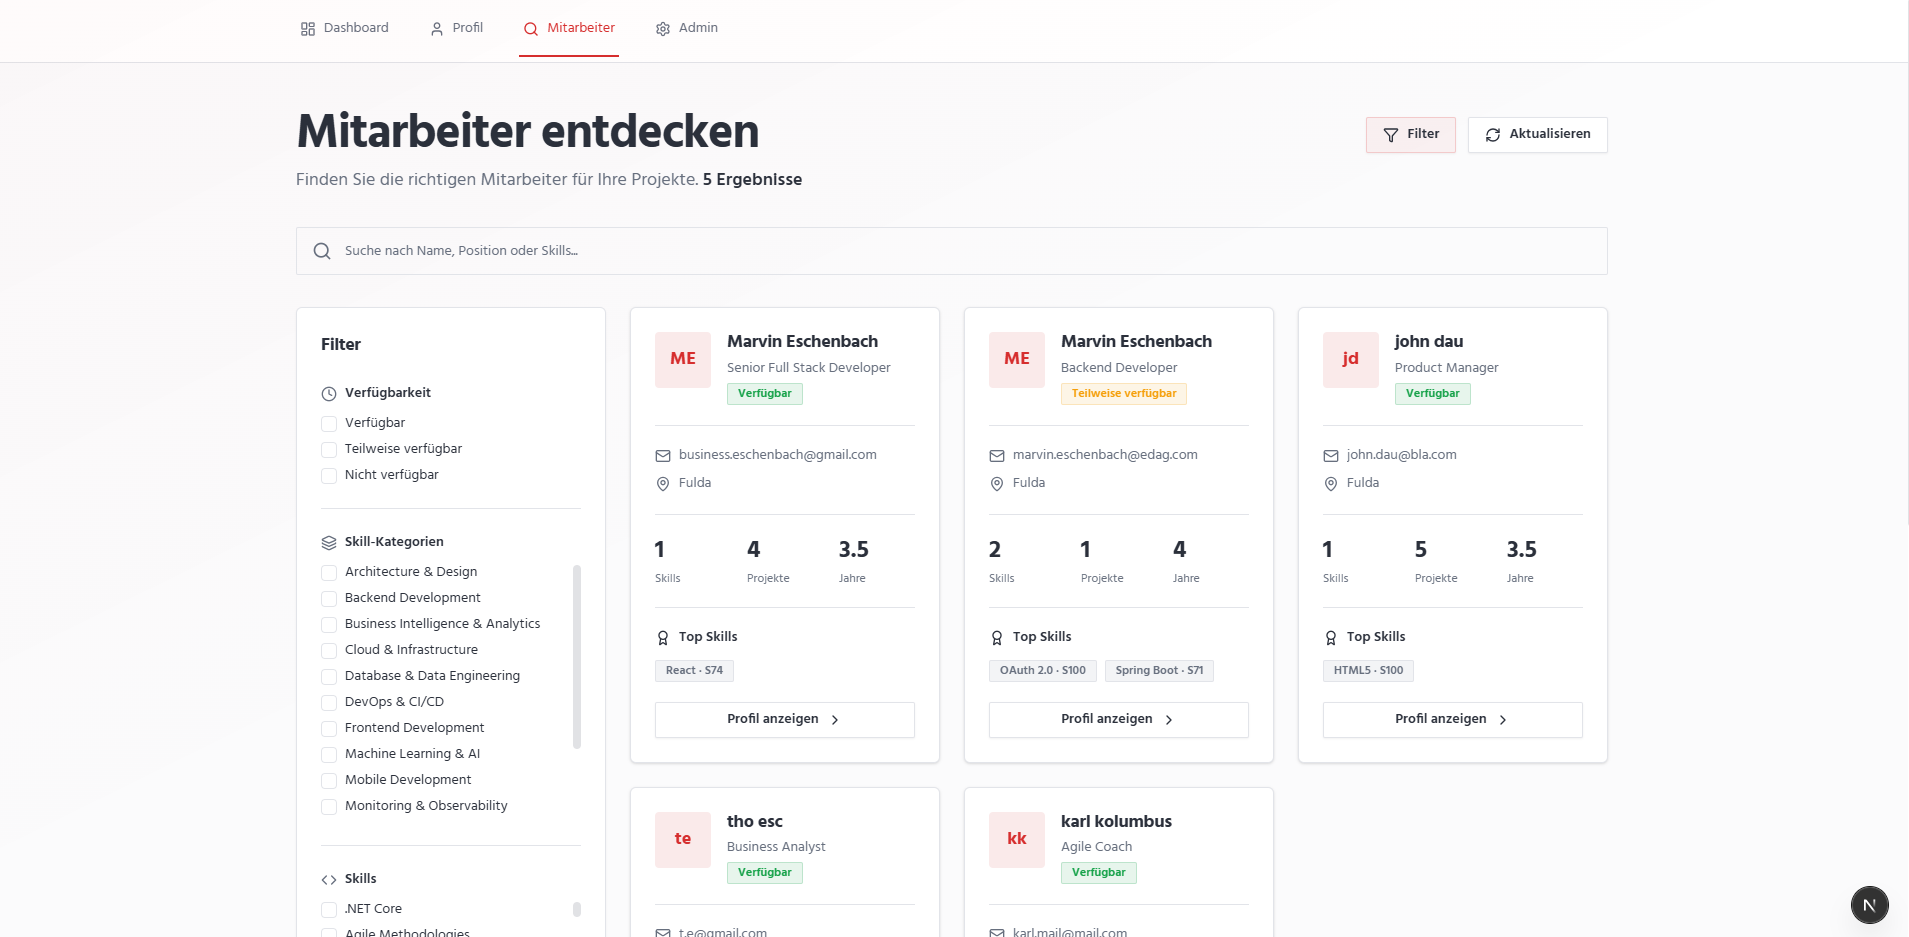
\includegraphics[width=\textwidth]{references/ui-employee-1.png}
\caption{Mitarbeitersuche mit Skill-basierten Filtern}
\label{fig:ui_employee_1}
\end{figure}

\begin{figure}[H]
\centering
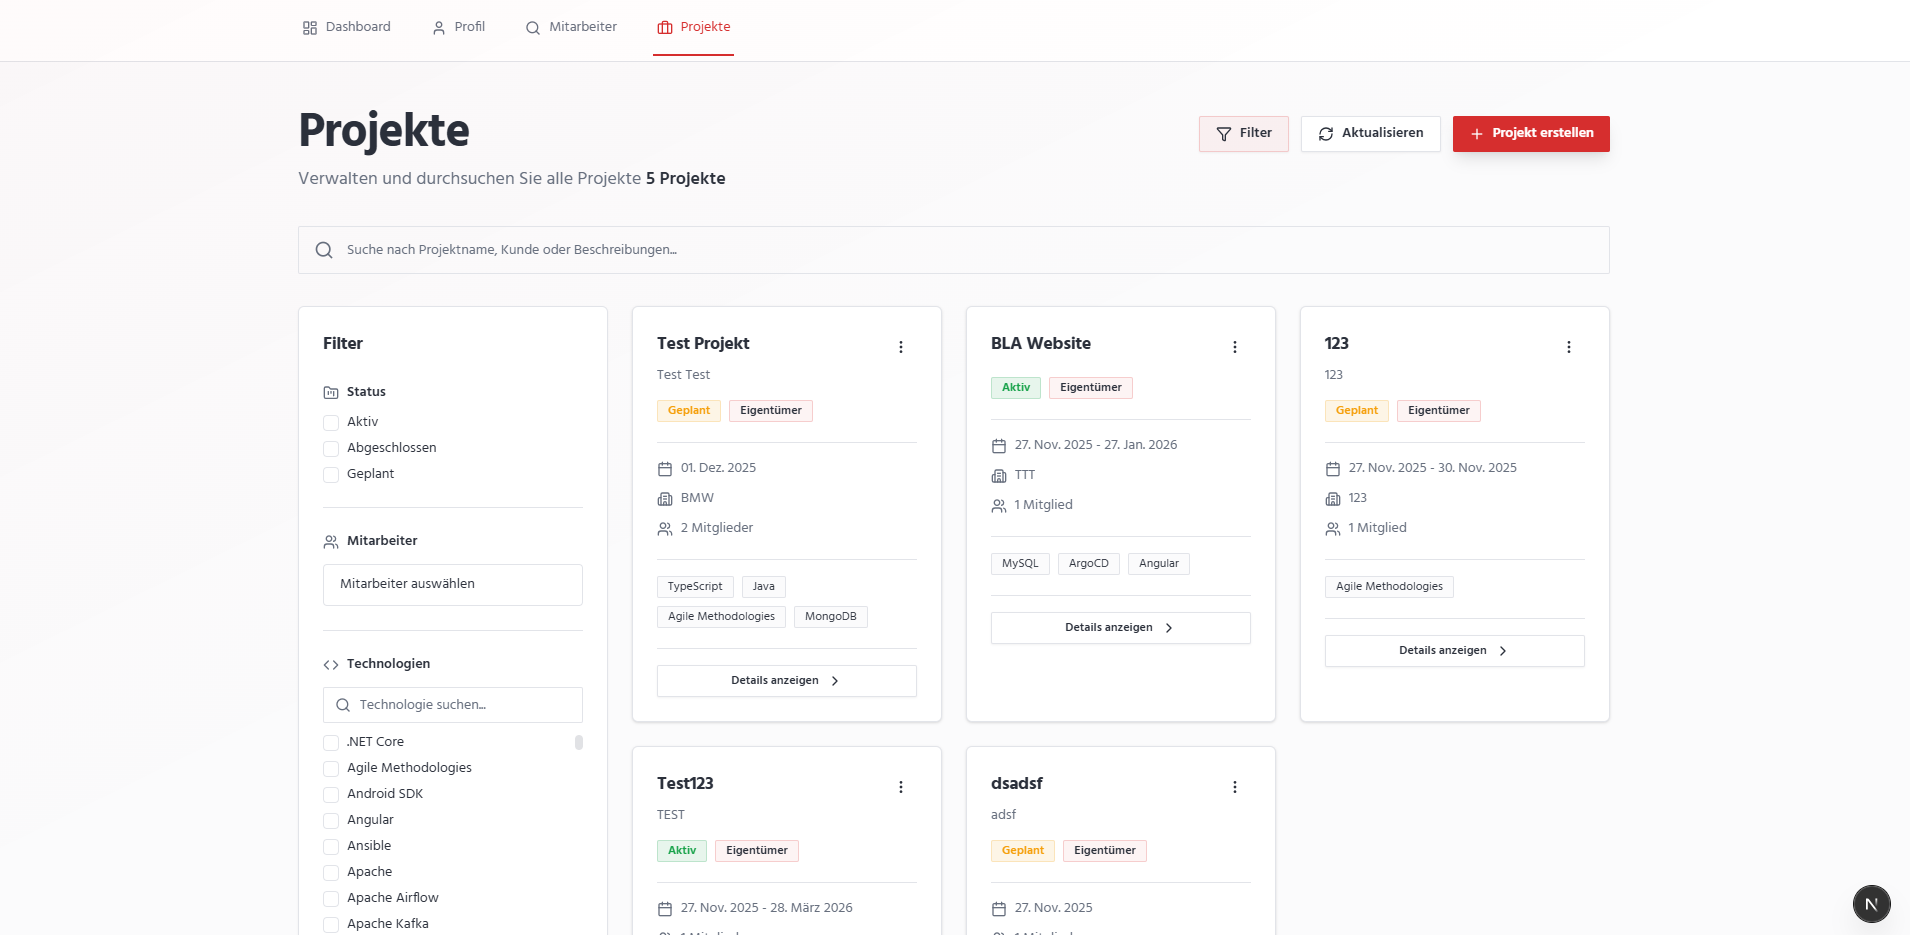
\includegraphics[width=\textwidth]{references/ui-projects-1.png}
\caption{Projektübersicht mit Status-Filter}
\label{fig:ui_projects_1}
\end{figure}

\begin{figure}[H]
\centering
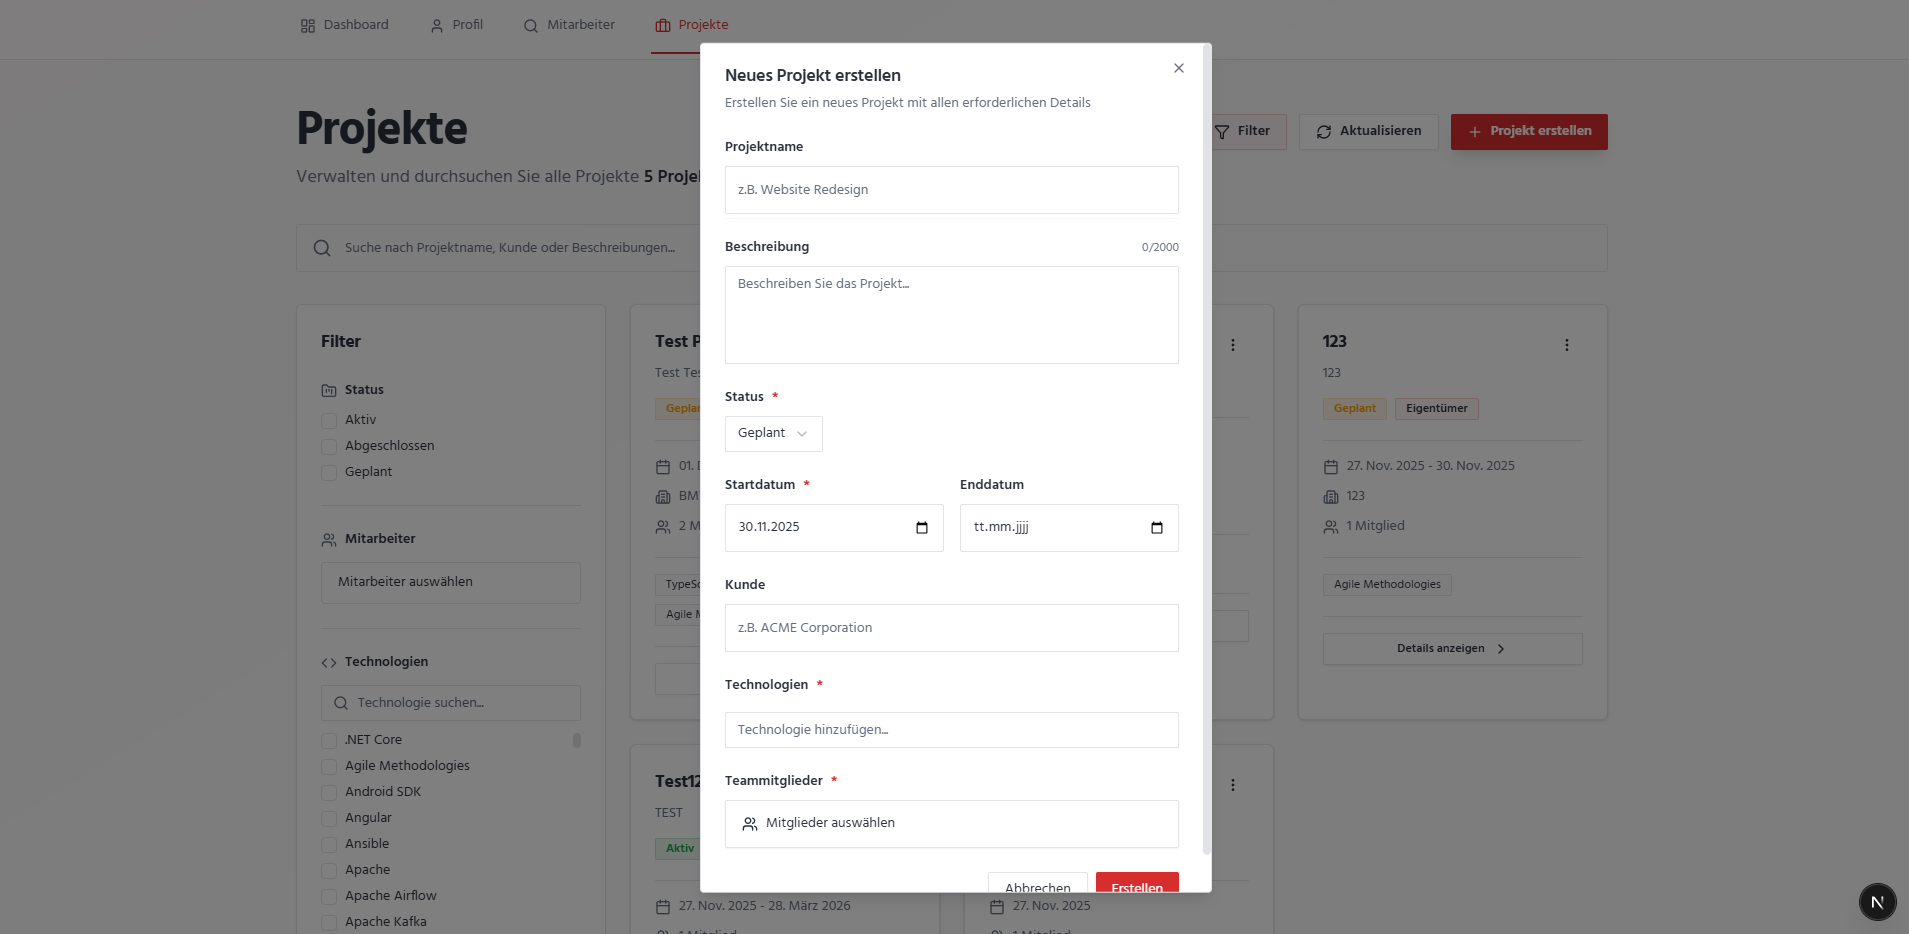
\includegraphics[width=\textwidth]{references/ui-projects-2.png}
\caption{Projekt-Detailansicht mit Team-Zusammensetzung}
\label{fig:ui_projects_2}
\end{figure}

\begin{figure}[H]
\centering
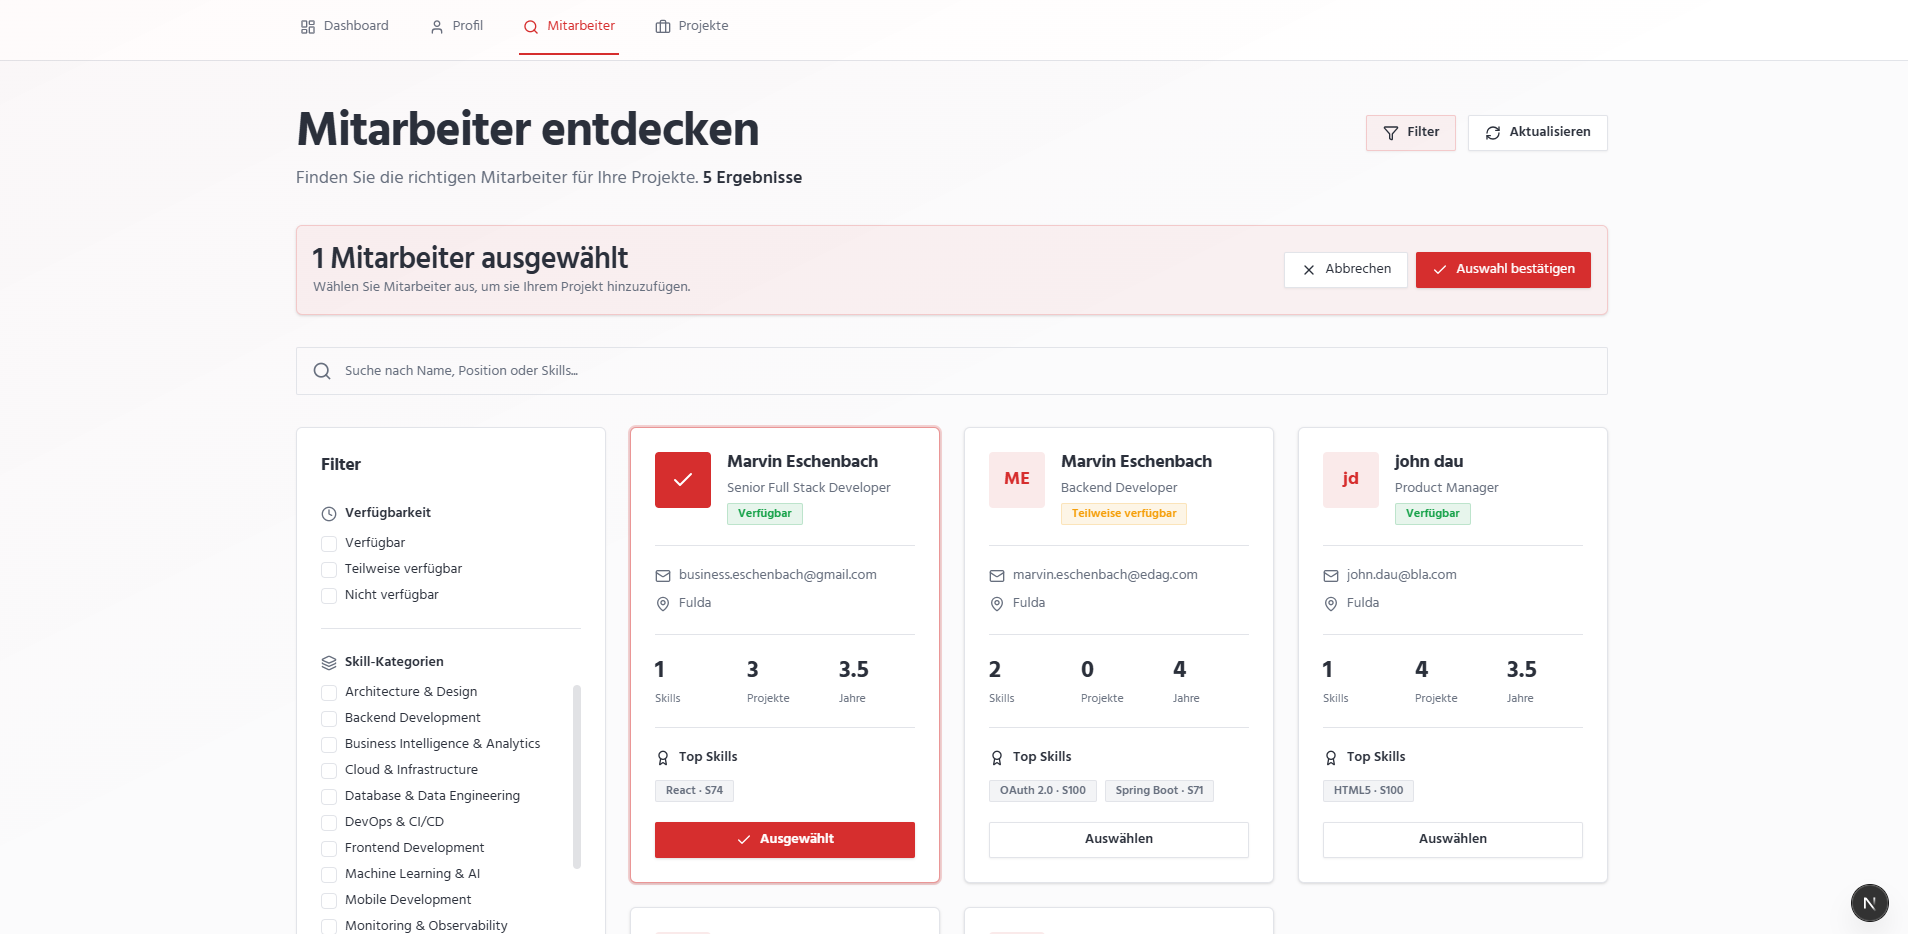
\includegraphics[width=\textwidth]{references/ui-projects-3.png}
\caption{Projekt-Erstellung: Formular für neue Projekte}
\label{fig:ui_projects_3}
\end{figure}

\begin{figure}[H]
\centering
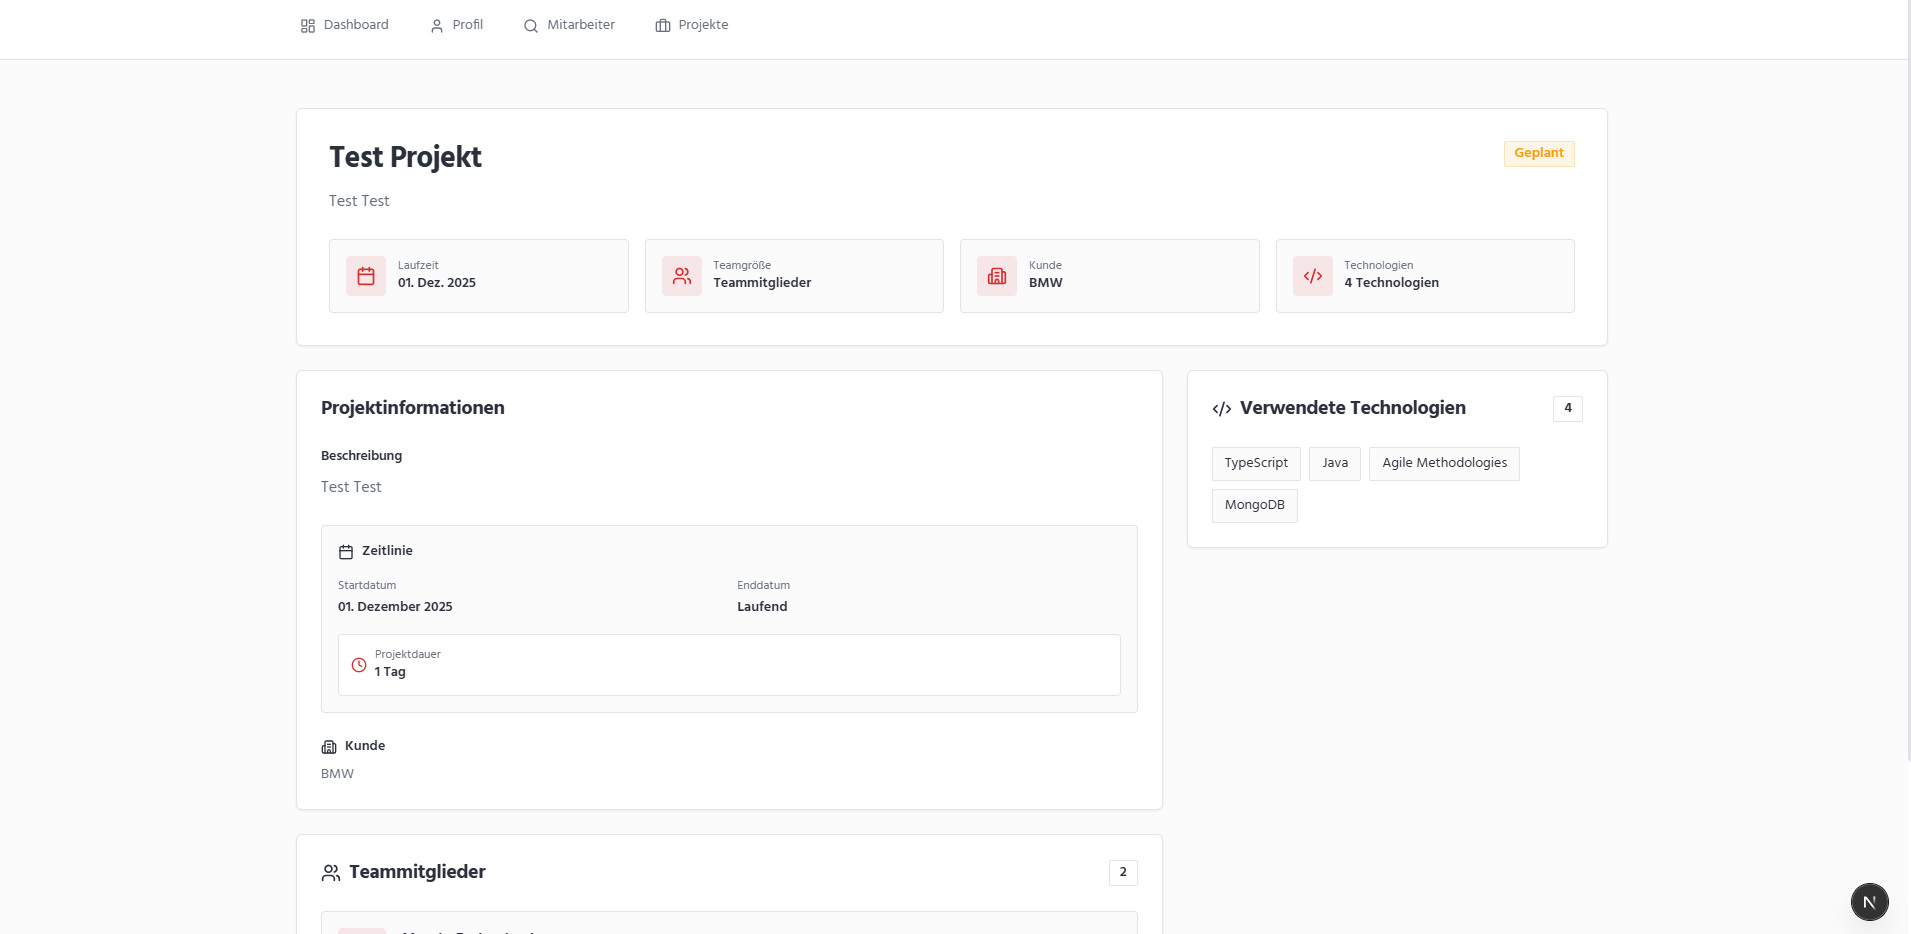
\includegraphics[width=\textwidth]{references/ui-projects-4.png}
\caption{Projekt-Team-Management: Mitglieder hinzufügen}
\label{fig:ui_projects_4}
\end{figure}

\subsubsection{Administrationsoberfläche}

\begin{figure}[H]
\centering
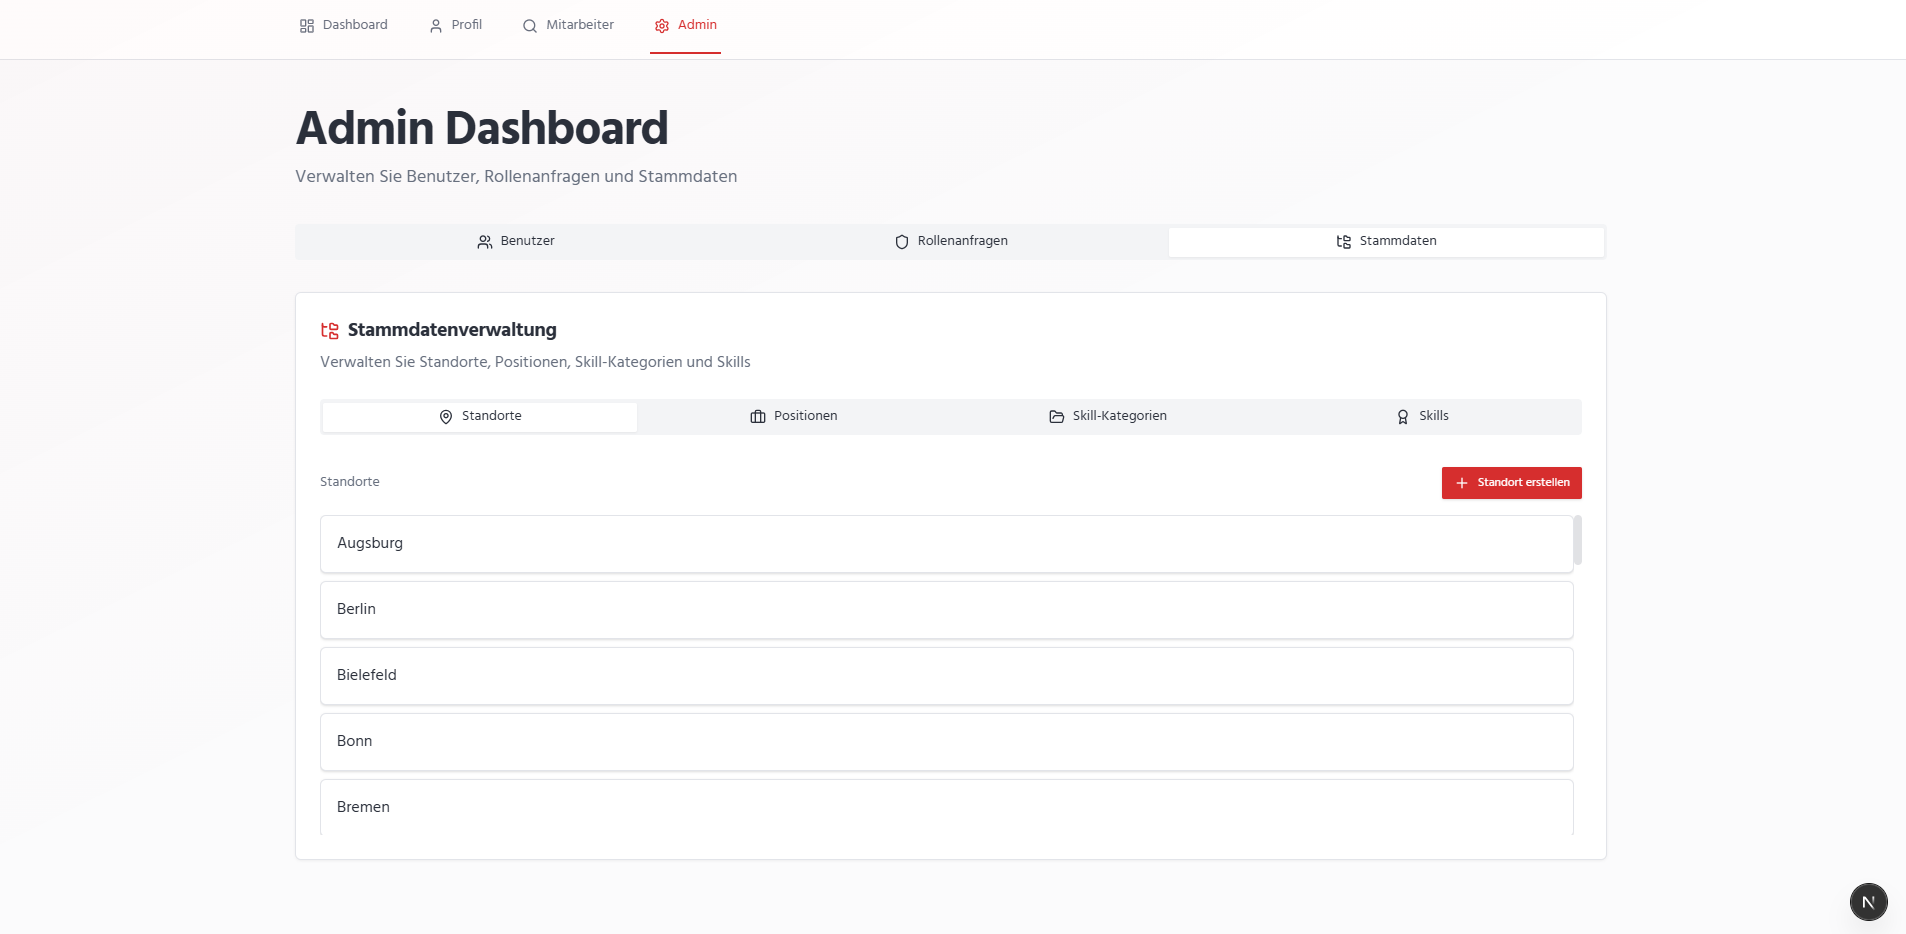
\includegraphics[width=\textwidth]{references/ui-admin-1.png}
\caption{Admin-Dashboard: Systemstatistiken und Benutzeraktivitäten}
\label{fig:ui_admin_1}
\end{figure}

\begin{figure}[H]
\centering
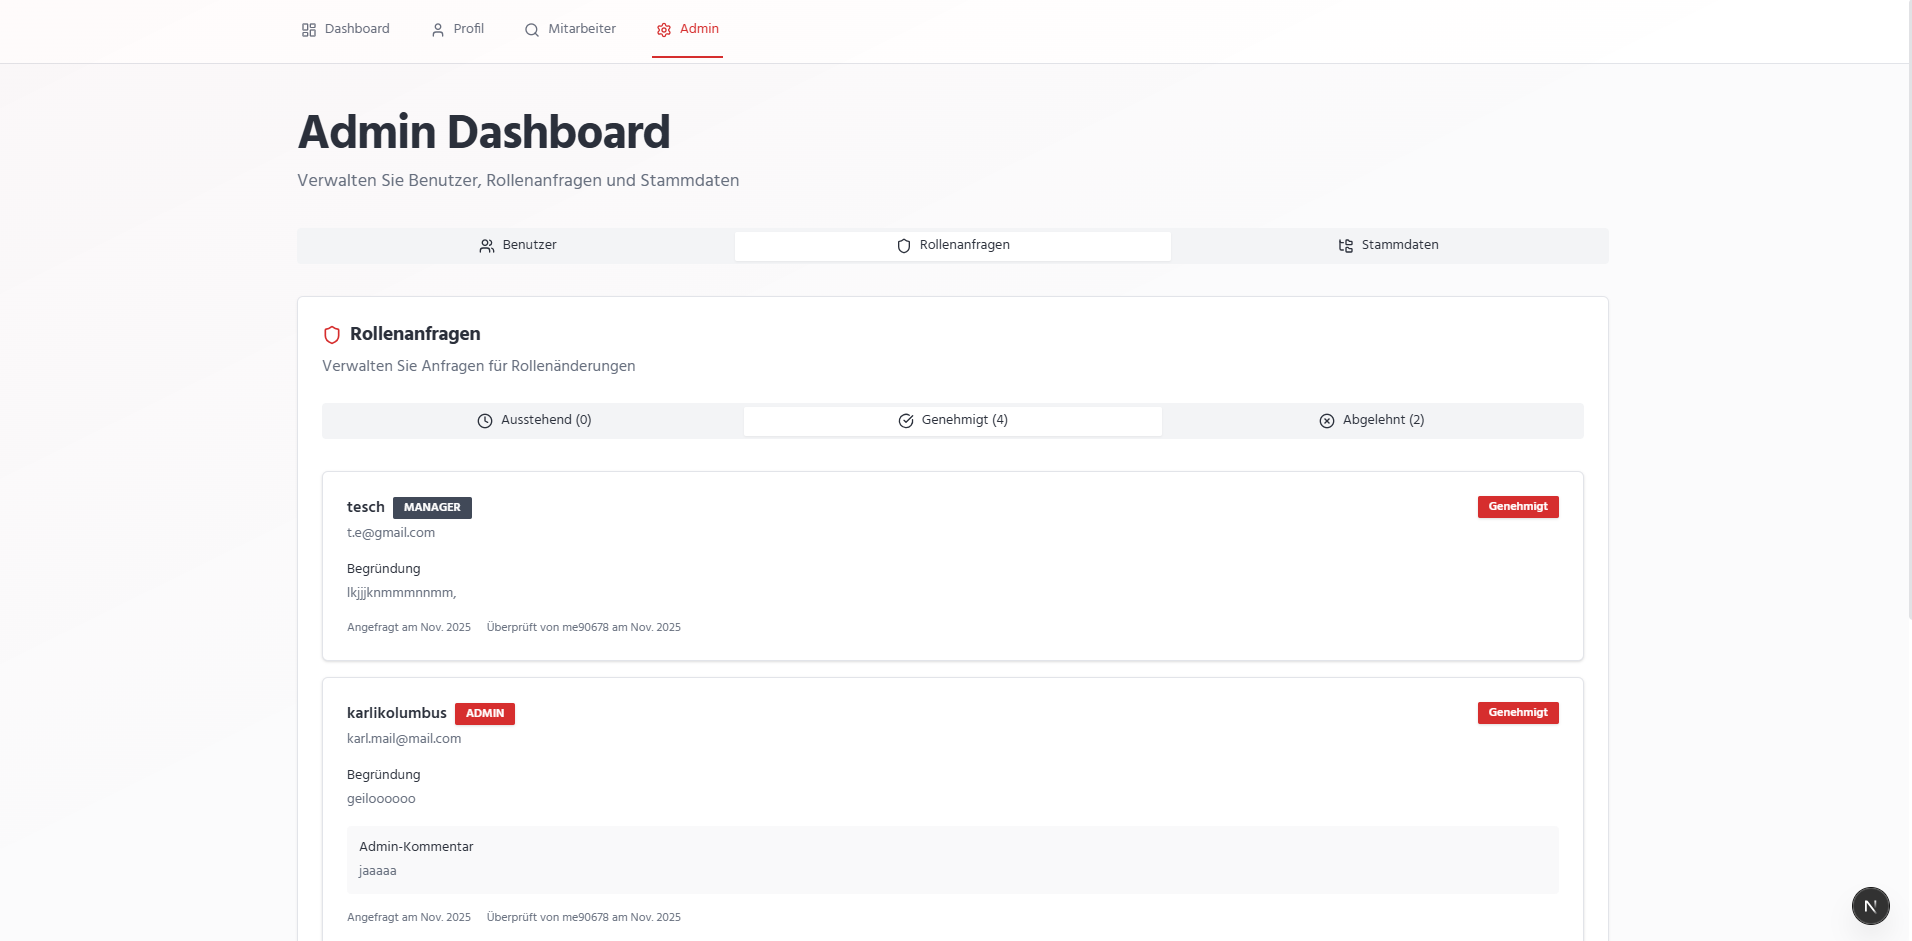
\includegraphics[width=\textwidth]{references/ui-admin-2.png}
\caption{Admin-Panel: Rollenanfragen-Verwaltung}
\label{fig:ui_admin_2}
\end{figure}

\subsubsection{UI-Mockup (Planungsphase)}

\begin{figure}[H]
\centering
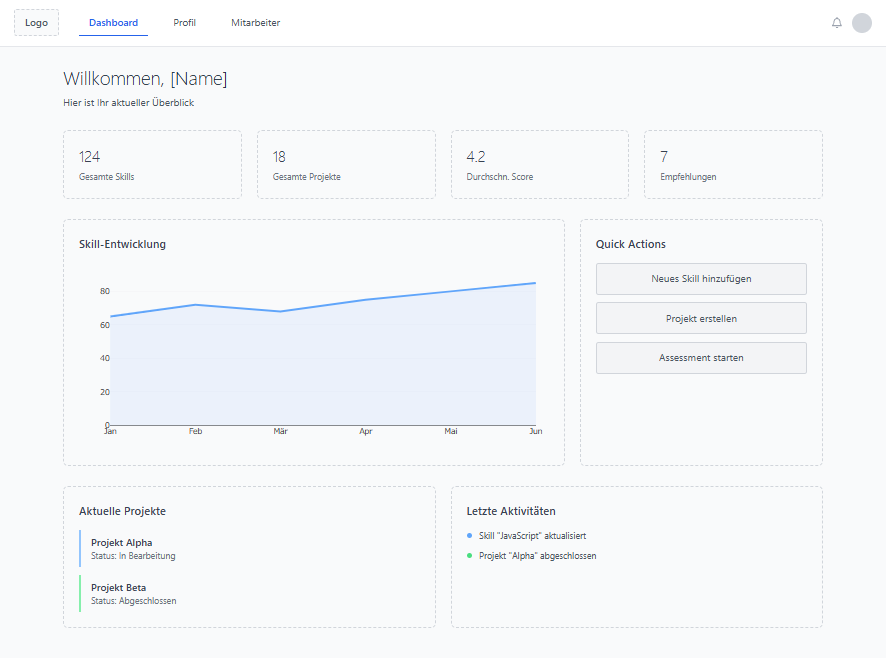
\includegraphics[width=\textwidth]{references/mockup-dashboard.png}
\caption{Initiales UI-Mockup aus der Planungsphase}
\label{fig:mockup_dashboard}
\end{figure}

\subsection{Use Cases}

\subsubsection{Übersicht der 15 implementierten Use Cases}

\begin{table}[H]
\centering
\footnotesize
\rowcolors{2}{EDAGDunkelgrau!10}{white}
\begin{tabularx}{\textwidth}{|l|X|p{2cm}|}
\hline
\rowcolor{EDAGDunkelgrau!10}
\textbf{Nr.} & \textbf{Use Case} & \textbf{Rolle} \\
\hline
UC-01 & Login über Keycloak OAuth2/OIDC & Alle \\
\hline
UC-02 & Eigenes Profil anzeigen und bearbeiten & USER \\
\hline
UC-03 & Skills hinzufügen/bearbeiten mit Proficiency Score & USER \\
\hline
UC-04 & Dashboard mit Skill-Entwicklung anzeigen & USER \\
\hline
UC-05 & Activity Feed anzeigen & USER \\
\hline
UC-06 & Mitarbeiter suchen (Multi-Filter) & USER \\
\hline
UC-07 & Projekte suchen & USER \\
\hline
UC-08 & Projekt anlegen mit Mitarbeiterauswahl & MANAGER \\
\hline
UC-09 & Projekt bearbeiten/Teammitglieder ändern & MANAGER \\
\hline
UC-10 & Projektdetails anzeigen & MANAGER \\
\hline
UC-11 & Rollenanfrage stellen (USER→MANAGER) & USER \\
\hline
UC-12 & Rollenanfrage genehmigen/ablehnen & ADMIN \\
\hline
UC-13 & Benutzerverwaltung (Rollenzuweisung) & ADMIN \\
\hline
UC-14 & Stammdaten verwalten (Skills, Kategorien) & ADMIN \\
\hline
UC-15 & Standorte verwalten & ADMIN \\
\hline
\end{tabularx}
\caption{Übersicht der 15 implementierten Use Cases}
\label{tab:use_cases}
\end{table}

\subsection{Benutzer- und Entwicklerdokumentation}

\begin{figure}[H]
\centering
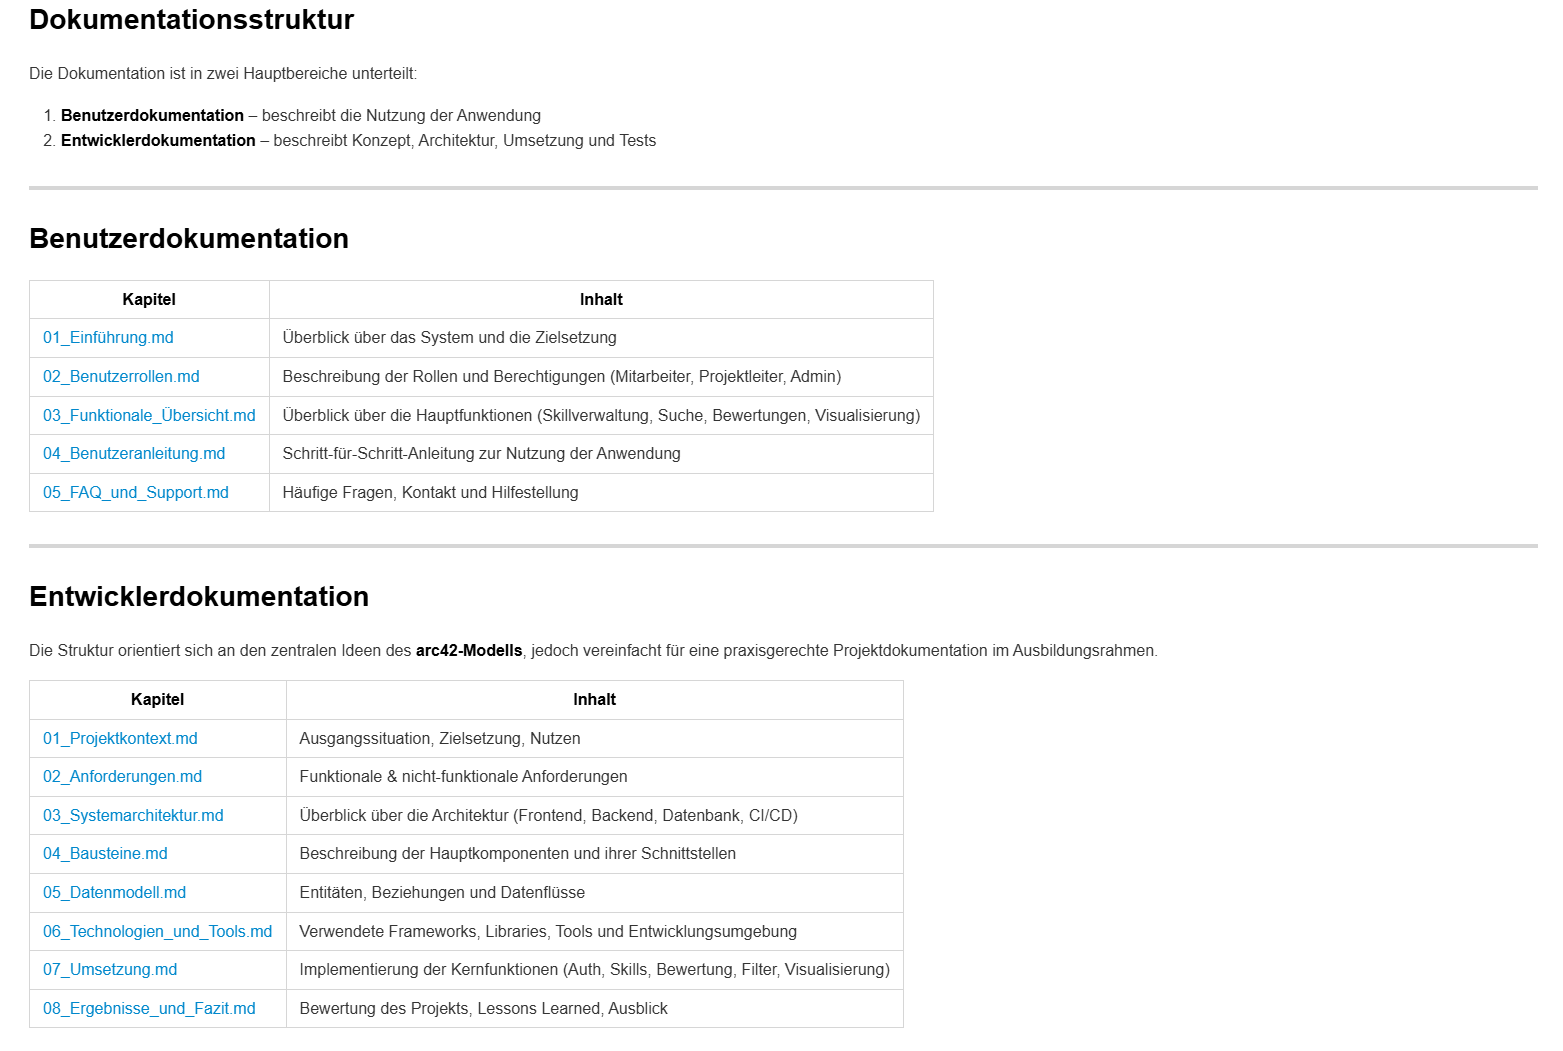
\includegraphics[width=\textwidth]{references/doc-1.png}
\caption{Benutzer- und Entwicklerdokumentation: Deckblatt der Benutzerdokumentation}
\label{fig:doc_user_guide}
\end{figure}

\begin{figure}[H]
\centering
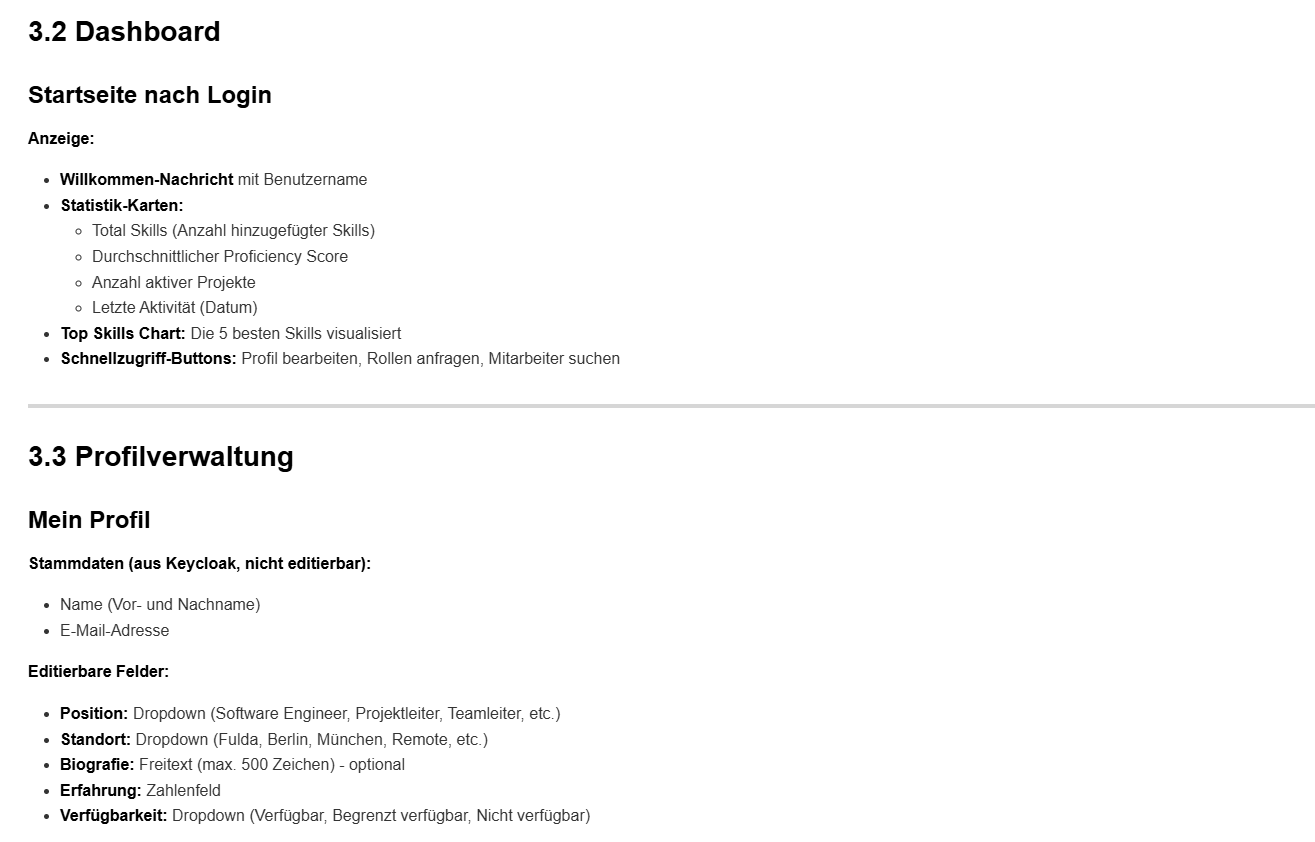
\includegraphics[width=\textwidth]{references/doc-2.png}
\caption{Benutzer- und Entwicklerdokumentation: Auszug aus der funktionalen Übersicht (Kapitel 3)}
\label{fig:doc_functional_overview}
\end{figure}

\begin{figure}[H]
\centering
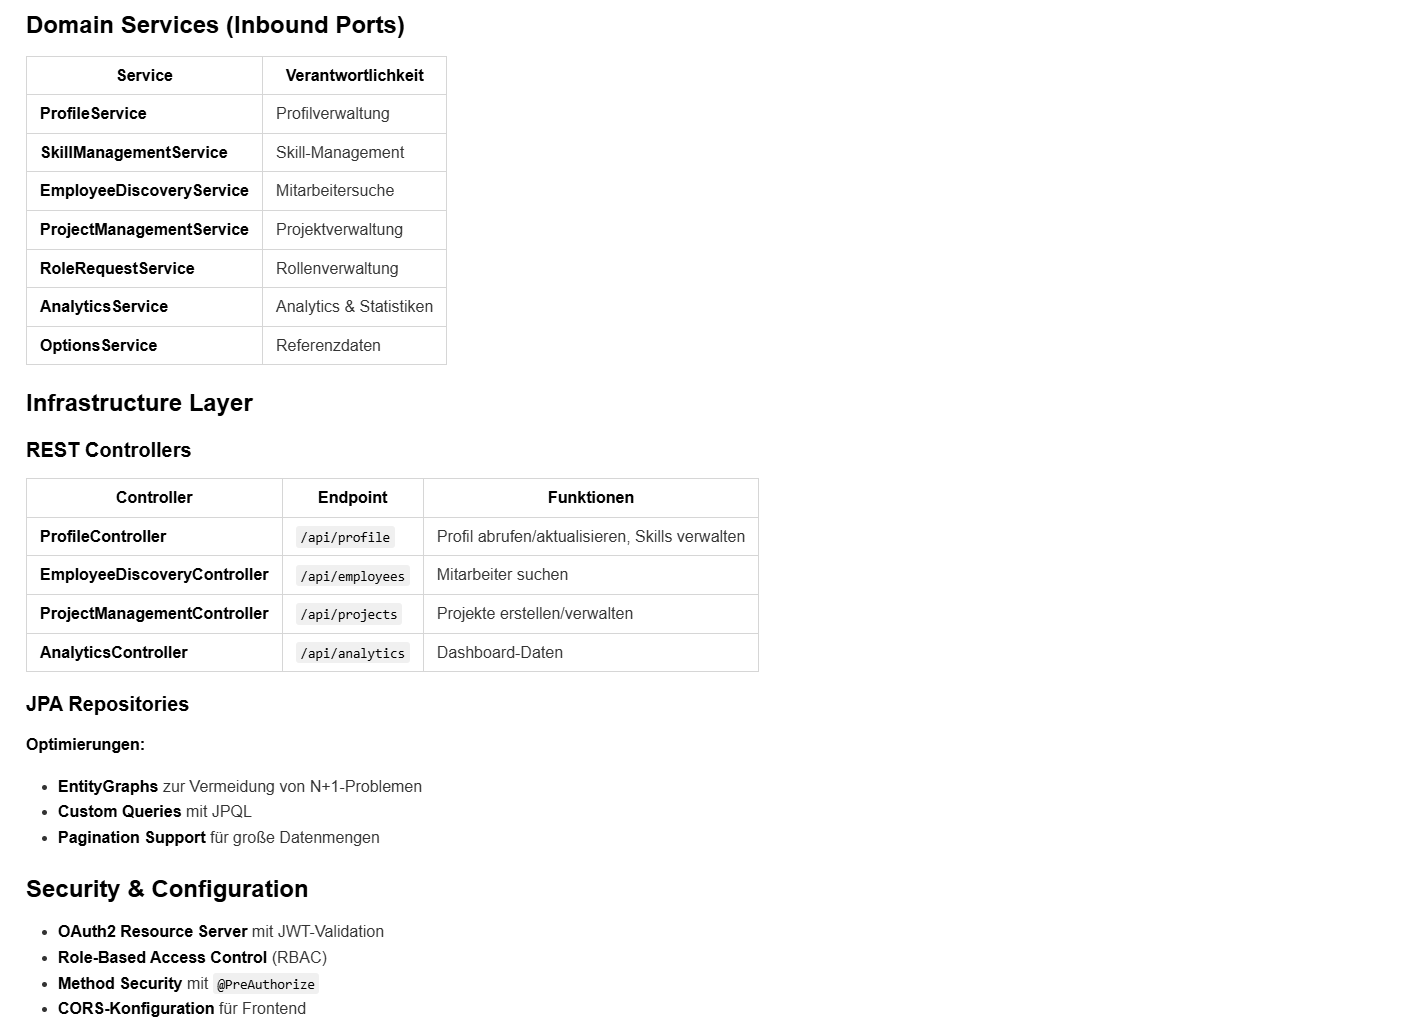
\includegraphics[width=\textwidth]{references/doc-3.png}
\caption{Benutzer- und Entwicklerdokumentation: Auszug aus der Architekturübersicht (Kapitel 4 - Bausteine)}
\label{fig:doc_architecture_blocks}
\end{figure}

Die Abbildungen~\ref{fig:doc_user_guide} bis~\ref{fig:doc_architecture_blocks} zeigen exemplarische Auszüge aus der erstellten Benutzer- und Entwicklerdokumentation, die eine umfassende Beschreibung aller Systemfunktionen, der technischen Architektur und der Deployment-Prozesse enthält.

\subsection{API-Dokumentation}
\label{sec:api_documentation}

Die REST-API des Skill Management Systems folgt RESTful-Prinzipien und ist vollständig mit OpenAPI 3.0 dokumentiert. Die API umfasst 7 Hauptbereiche mit insgesamt über 30 Endpunkten für Profilverwaltung, Mitarbeitersuche, Projektmanagement, Administration und Analytics.

\begin{figure}[H]
\centering
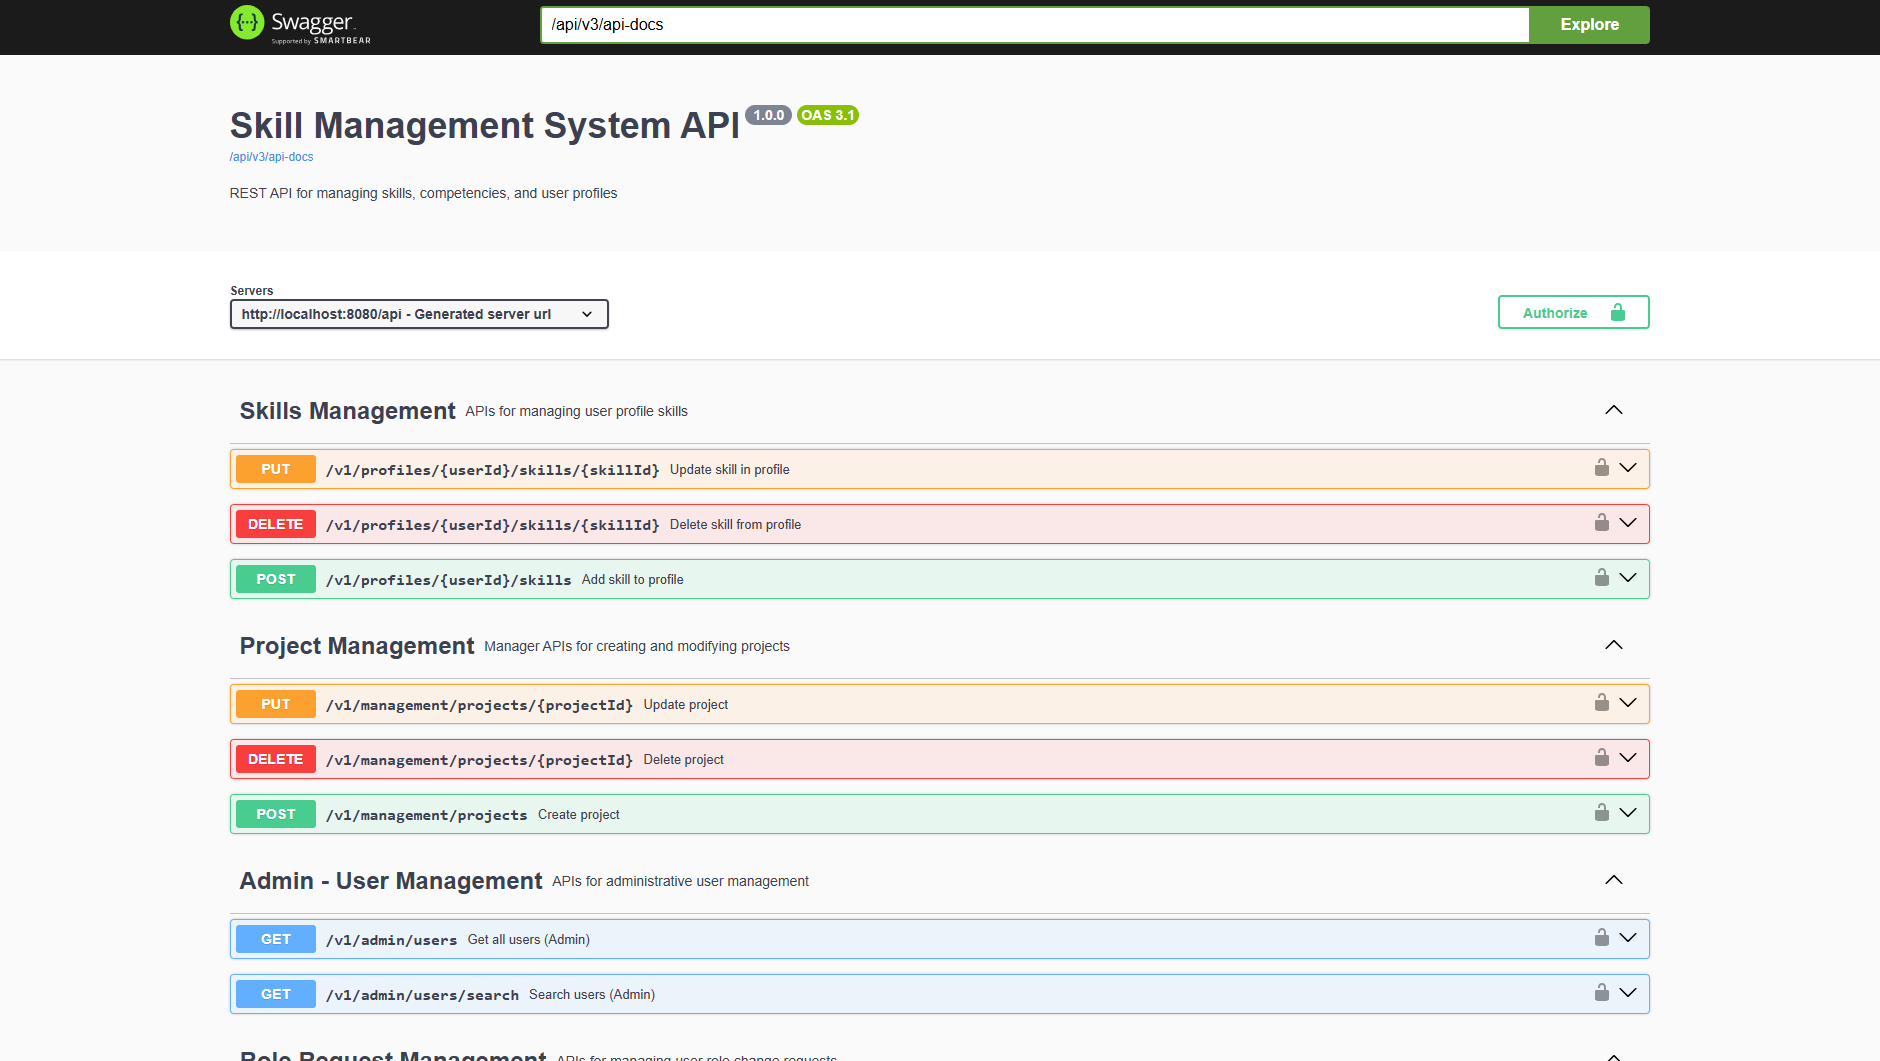
\includegraphics[width=\textwidth]{references/schnittstellen-doku-1.png}
\caption{API-Dokumentation: Übersicht der verfügbaren Endpunkte gruppiert nach Funktionsbereichen}
\label{fig:api_documentation}
\end{figure}

\subsubsection{Vollständige API-Endpunkt-Übersicht}

Die folgende Tabelle listet alle implementierten API-Endpunkte mit HTTP-Methode, Pfad, Beschreibung und erforderlicher Rolle auf:

\begin{table}[H]
\centering
\tiny
\rowcolors{2}{EDAGDunkelgrau!10}{white}
\begin{tabularx}{\textwidth}{|l|l|X|l|}
\hline
\rowcolor{EDAGDunkelgrau!30}
\textbf{Methode} & \textbf{Endpunkt} & \textbf{Beschreibung} & \textbf{Rolle} \\
\hline
\multicolumn{4}{|l|}{\cellcolor{EDAGDunkelgrau!10}\textbf{Skills Management}} \\
\hline
PUT & /v1/profiles/\{userId\}/skills/\{skillId\} & Update skill in profile & USER \\
\hline
DELETE & /v1/profiles/\{userId\}/skills/\{skillId\} & Delete skill from profile & USER \\
\hline
POST & /v1/profiles/\{userId\}/skills & Add skill to profile & USER \\
\hline

\multicolumn{4}{|l|}{\cellcolor{EDAGDunkelgrau!10}\textbf{Project Management}} \\
\hline
PUT & /v1/management/projects/\{projectId\} & Update project & MANAGER \\
\hline
DELETE & /v1/management/projects/\{projectId\} & Delete project & MANAGER \\
\hline
POST & /v1/management/projects & Create project & MANAGER \\
\hline

\multicolumn{4}{|l|}{\cellcolor{EDAGDunkelgrau!10}\textbf{Admin - User Management}} \\
\hline
GET & /v1/admin/users & Get all users (Admin) & ADMIN \\
\hline
GET & /v1/admin/users/search & Search users (Admin) & ADMIN \\
\hline

\multicolumn{4}{|l|}{\cellcolor{EDAGDunkelgrau!10}\textbf{Role Request Management}} \\
\hline
GET & /v1/role-requests & Get role requests by status & USER \\
\hline
POST & /v1/role-requests & Create role request & USER \\
\hline
POST & /v1/role-requests/\{requestId\}/reject & Reject role request & ADMIN \\
\hline
POST & /v1/role-requests/\{requestId\}/approve & Approve role request & ADMIN \\
\hline
GET & /v1/role-requests/me & Get my role requests & USER \\
\hline
DELETE & /v1/role-requests/\{requestId\} & Cancel role request & USER \\
\hline

\multicolumn{4}{|l|}{\cellcolor{EDAGDunkelgrau!10}\textbf{Profile Management}} \\
\hline
GET & /v1/profiles/\{userId\} & Get user profile & USER \\
\hline
PUT & /v1/profiles/\{userId\} & Update user profile & USER \\
\hline

\multicolumn{4}{|l|}{\cellcolor{EDAGDunkelgrau!10}\textbf{Employee Discovery}} \\
\hline
GET & /v1/employees/\{userId\} & Get employee by ID & USER \\
\hline
GET & /v1/employees/search & Search employees & USER \\
\hline
GET & /v1/employees/filter-options & Get filter options & USER \\
\hline

\multicolumn{4}{|l|}{\cellcolor{EDAGDunkelgrau!10}\textbf{Projects}} \\
\hline
GET & /v1/projects/\{projectId\} & Get project by ID & USER \\
\hline
GET & /v1/projects/users/\{userId\} & Get user projects & USER \\
\hline
GET & /v1/projects/search & Search manager's projects & MANAGER \\
\hline
GET & /v1/projects/filter-options & Get project filter options & USER \\
\hline

\multicolumn{4}{|l|}{\cellcolor{EDAGDunkelgrau!10}\textbf{Analytics \& Activities}} \\
\hline
GET & /v1/analytics/users/\{userId\}/statistics & Get user statistics & USER \\
\hline
GET & /v1/analytics/users/\{userId\}/skill-trends & Get skill development trends & USER \\
\hline
GET & /v1/analytics/users/\{userId\}/activities & Get recent activities & USER \\
\hline

\multicolumn{4}{|l|}{\cellcolor{EDAGDunkelgrau!10}\textbf{Reference Data Options}} \\
\hline
GET & /v1/options/skills & Get all available skills & USER \\
\hline
POST & /v1/options/skills & Create skill (Admin) & ADMIN \\
\hline
GET & /v1/options/skill-categories & Get skill categories & USER \\
\hline
POST & /v1/options/skill-categories & Create skill category (Admin) & ADMIN \\
\hline
GET & /v1/options/positions & Get available positions & USER \\
\hline
POST & /v1/options/positions & Create position (Admin) & ADMIN \\
\hline
GET & /v1/options/locations & Get available locations & USER \\
\hline
POST & /v1/options/locations & Create location (Admin) & ADMIN \\
\hline
GET & /v1/options/skills/category/\{categoryId\} & Get available skills by category & USER \\
\hline
\end{tabularx}
\caption{Vollständige REST-API-Endpunkt-Übersicht des Skill Management Systems}
\label{tab:api_endpoints}
\end{table}

\textbf{Authentifizierung:} Alle Endpunkte erfordern einen gültigen JWT Access Token im Authorization-Header (\texttt{Bearer <token>}). Die Token-Validierung erfolgt via Keycloak Token Introspection (siehe Sequenzdiagramm in Abbildung~\ref{fig:auth_sequence}).


% ==========================================
% Literaturverzeichnis
% ==========================================
\printbibliography[heading=bibintoc, title={Literaturverzeichnis}]

\end{document}
